\documentclass[aspectratio=169,10pt]{beamer}
\usetheme{default}\usecolortheme{default}
\setbeamertemplate{navigation symbols}{}
\setbeamertemplate{footline}[frame number]
\usepackage{booktabs}\usepackage{graphicx}\usepackage{hyperref}\usepackage{array}
\hypersetup{colorlinks=true,urlcolor=blue!60!black,linkcolor=black}
\title{SBND DL vertexing on data: Xin round 2 vs \texttt{original} vs \texttt{aurora\_space}}
\subtitle{nueCC-48 + NC$\pi^0$-19, against Xin's round-2 hand scan}
\author{Haiwang Yu (prepared with Claude Code)}
\date{2026-11-16}
\begin{document}
\frame{\titlepage}

\begin{frame}{Setup: the three methods}
\small
\begin{tabular}{>{\raggedright\arraybackslash}p{0.13\linewidth}>{\raggedright\arraybackslash}p{0.82\linewidth}}
\toprule
\textbf{Xin r2} & Xin's \emph{prod0811} delivery (2026-08-11) behind the round-2 hand-scan Bee sets (\texttt{9e2a1a1e} nueCC, \texttt{13900b8c} NC$\pi^0$).
His 2-step chain: stage A = \texttt{cb0805} Q/L hubs (toolkit \texttt{a1ea3789}); stage B = \texttt{run\_pr\_chain\_batch.sh \ldots{} data} at toolkit \texttt{b38127a0}
(apply-pointcloud, ``pr/64 round 4''), compiled defaults. uboone SCN DL vertex, \emph{single} chain (no dual chain, no \texttt{vertex\_method}).
Main vertex: Bee neutrino-vertex marker. Scores: \emph{not recoverable} (\texttt{tracking-pr.root} deleted 2026-08-13). \\
\midrule
\textbf{original} & WCT master \texttt{c6be329e} + PR\,\#547 (tree of \texttt{e426d988}); \texttt{vertex\_method=original}: uboone SCN net
(\texttt{t48k-m16-l5-lr5d-res0.5-CP24.pth}), re-rank top-5 (accept score $\ge 10$), dual chain \texttt{snap} (transfer $\le 2$\,cm), fit exclusion,
\texttt{improve\_vertex} and the snap/audit refinements. 2 network calls per candidate. \\
\midrule
\textbf{aurora} & Same build; \texttt{vertex\_method=dv2\_split\_move}, bundle \texttt{dv2max/sbnd/aurora\_space} (wire-cell-data \#8, \texttt{bundle.json} sha256 \texttt{51588842}):
DV2-MAX trained on aurora-r2 MC (478k events), input = trajectory-fit cloud + Bee space points of touching clusters; vertex = nearest graph vertex if
$<1.5$\,cm, else split at the nearest fit point, then moved onto the DV2-MAX point. No dual chain. 1 call per candidate. \\
\bottomrule
\end{tabular}

\medskip
Both of our arms: step 2 from the same step-1 tars (\#43 data slices, FrameShift applied), production data TLAs, one pinned core each.
\end{frame}

\begin{frame}{Links}
\small
\begin{itemize}
\item Tracking issue: \href{https://github.com/HaiwangYu/wire-cell-toolkit-ai-helper/issues/47}{ai-helper \#47}; space-point plan \href{https://github.com/HaiwangYu/wire-cell-toolkit-ai-helper/issues/44}{\#44};
DL dump \href{https://github.com/HaiwangYu/wire-cell-toolkit-ai-helper/issues/35}{\#35}; PR\,\#543 review \href{https://github.com/HaiwangYu/wire-cell-toolkit-ai-helper/issues/43}{\#43}; flat CAF \href{https://github.com/HaiwangYu/wire-cell-toolkit-ai-helper/issues/39}{\#39}; truth match \href{https://github.com/HaiwangYu/wire-cell-toolkit-ai-helper/issues/41}{\#41}
\item WCT PRs: \href{https://github.com/WireCell/wire-cell-toolkit/pull/543}{\#543} (DV2-MAX, merged),
\href{https://github.com/WireCell/wire-cell-toolkit/pull/544}{\#544} (flat CAF + truth match, merged),
\href{https://github.com/WireCell/wire-cell-toolkit/pull/547}{\#547} (\texttt{aurora\_space}, open);
wire-cell-data \href{https://github.com/WireCell/wire-cell-data/pull/8}{\#8} (bundle, merged)
\item Docs (issue-47 folder): \href{https://github.com/HaiwangYu/wire-cell-toolkit-ai-helper/blob/main/issues/47-dv2max-aurora-space-model/porting_sbndbuild03/data-orig-vs-aur.md}{data original vs aurora},
\href{https://github.com/HaiwangYu/wire-cell-toolkit-ai-helper/blob/main/issues/47-dv2max-aurora-space-model/prod_polaris/handscan-vertex.md}{hand-scan vertex method},
\href{https://github.com/HaiwangYu/wire-cell-toolkit-ai-helper/blob/main/issues/47-dv2max-aurora-space-model/prod_polaris/data-events-handscan.md}{per-event table},
\href{https://github.com/HaiwangYu/wire-cell-toolkit-ai-helper/blob/main/issues/47-dv2max-aurora-space-model/porting_sbndbuild03/results.md}{MC + hold-out validation}
\item Bee: \href{https://www.phy.bnl.gov/twister/bee/set/89cdea53-c227-476c-8f67-0ae765f804b4/event/0/}{original set}, \href{https://www.phy.bnl.gov/twister/bee/set/431dc57f-997d-4cff-88e1-4e33fd743ab8/event/0/}{aurora set};
Xin r2 \href{https://www.phy.bnl.gov/twister/bee/set/9e2a1a1e-b637-4be5-99b7-f49bf8c04c57/event/0/}{nueCC},
\href{https://www.phy.bnl.gov/twister/bee/set/13900b8c-e48c-4ebb-8daa-da19e2e989b6/event/0/}{NC$\pi^0$}
\end{itemize}
\end{frame}

\begin{frame}{Hand-scan reference (``true'' vertex in this deck)}
\small
\begin{itemize}
\item Xin's round-2 hand scan rates each event's round-2 vertex: Good / OK / Not OK / Not good.
\item \textbf{Good/OK}: reference = Xin r2's main vertex (the neutrino-vertex marker of his Bee set).
So Xin r2 is 0\,cm \emph{by construction} on these events.
\item \textbf{Not OK/Not good with ``(x, y, z)''}: reference = the scanner's point (eyeballed in Bee, $\sim$1\,cm).
\item Excluded from the vertex numbers: 3 ``Not good'' events without coordinates; 5 events where our selected candidate is a different interaction from
the scanned one (both our arms $>10$\,cm away and within 0.2\,cm of each other); 1 event not in the sheet (18259/1/116962).
\item Two sheet RSE typos corrected against Xin's Bee events (18255-234538$\to$234638, 18355-40074$\to$400474).
\item Flavor: from the hand-picked sample (nueCC-48 $\to\nu_e$CC, NC$\pi^0$-19 $\to$ NC$\pi^0$), with the scanner's note when it suggests otherwise.
\item Prediction from scores: $\nu_e$ = \texttt{nue\_score} $>7$; $\nu_\mu$CC = \texttt{numu\_score} $>0.9$; ``no $\nu$'' = fails the generic cut.
\end{itemize}
\end{frame}

\begin{frame}{Vertexing vs the hand scan (assumed true)}
\scriptsize
Entries: $<1$/$<2$/$<3$\,cm of $n$ events, median distance [cm].
\begin{center}
\begin{tabular}{llccc}
\toprule
sample & reference & Xin r2 & original & aurora \\
\midrule
$\nu_e$CC-48 & scan Good/OK & 34/34/34 of 34, 0.00 & 28/31/32 of 34, 0.39 & 30/31/33 of 34, 0.31 \\
$\nu_e$CC-48 & scan Not good & 0/0/0 of 8, 45.77 & 4/6/6 of 8, 1.06 & 5/7/8 of 8, 0.80 \\
$\nu_e$CC-48 & all & 34/34/34 of 42, 0.00 & 32/37/38 of 42, 0.43 & 35/38/41 of 42, 0.36 \\
NC$\pi^0$-19 & scan Good/OK & 11/11/11 of 11, 0.00 & 5/5/8 of 11, 2.32 & 5/8/9 of 11, 1.05 \\
NC$\pi^0$-19 & scan Not good & 0/0/0 of 5, 105.90 & 0/0/0 of 5, 25.55 & 3/4/4 of 5, 0.94 \\
NC$\pi^0$-19 & all & 11/11/11 of 16, 0.00 & 5/5/8 of 16, 3.23 & 8/12/13 of 16, 1.00 \\
all & scan Good/OK & 45/45/45 of 45, 0.00 & 33/36/40 of 45, 0.43 & 35/39/42 of 45, 0.35 \\
all & scan Not good & 0/0/0 of 13, 59.93 & 4/6/6 of 13, 5.15 & 8/11/12 of 13, 0.93 \\
all & all & 45/45/45 of 58, 0.00 & 37/42/46 of 58, 0.59 & 43/50/54 of 58, 0.52 \\
\bottomrule
\end{tabular}
\end{center}
\begin{itemize}
\item Where the scanners located the right vertex (Not good), \textbf{aurora} is within 1.5\,cm in 11 of 13 events; \textbf{original} is 5--50\,cm off in 7.
\item Where Xin r2 was judged Good/OK, aurora is at least as close to that vertex as original (the reference is biased towards Xin r2, and partly towards original).
\end{itemize}
\end{frame}

\begin{frame}{Predictions from the current scores}
\small
\begin{center}
\begin{tabular}{llccccc}
\toprule
sample (hand-scan flavor) & method & $\nu_e$ & $\nu_\mu$CC & both & other & no $\nu$ \\
\midrule
nueCC-48 ($\nu_e$CC) & Xin r2 & \multicolumn{5}{c}{scores not recoverable} \\
nueCC-48 ($\nu_e$CC) & original & 37 & 4 & 1 & 6 & 0 \\
nueCC-48 ($\nu_e$CC) & aurora & 40 & 3 & 1 & 4 & 0 \\
\midrule
NC$\pi^0$-19 (NC) & Xin r2 & \multicolumn{5}{c}{scores not recoverable} \\
NC$\pi^0$-19 (NC) & original & 1 & 2 & 0 & 16 & 0 \\
NC$\pi^0$-19 (NC) & aurora & 1 & 1 & 0 & 17 & 0 \\
\bottomrule
\end{tabular}
\end{center}
\begin{itemize}
\item $\nu_e$: \texttt{nue\_score} $>7$; $\nu_\mu$CC: \texttt{numu\_score} $>0.9$; both: passes both; other: neither; no $\nu$: fails the generic cut.
\item nueCC-48 is hand-scanned $\nu_e$CC, so more $\nu_e$ is better. NC$\pi^0$-19 is NC, so $\nu_e$ or $\nu_\mu$CC there is wrong.
\item original $\to$ aurora: 9 events change; the per-event pages flag them.
\end{itemize}
\end{frame}

\begin{frame}{nueCC-48: 18255/1/271851}
\vspace{-6pt}
\centering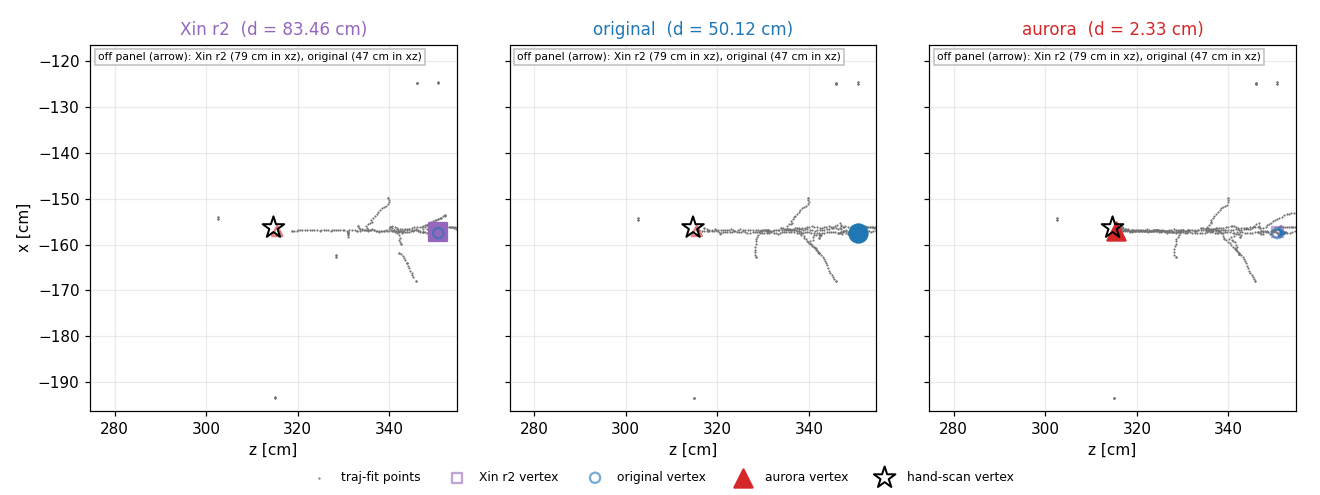
\includegraphics[width=0.92\linewidth]{figures/evt-18255-271851.png}\\[-2pt]
\scriptsize\raggedright
\textbf{Hand scan:} vertex (-156.3, 6.4, 314.7) [scanner point], Xin r2 verdict: Not good, flavor: $\nu_e$CC; \textcolor{red}{selection changes}\\
\textit{Scan note: close to (x, y, z) = (-156.3, 6.4, 314.7)}\\
\begin{tabular}{llcccc}
\toprule
method & & main vertex (x, y, z) cm & d to hand scan [cm] & $\nu_e$ / $\nu_\mu$ score & prediction \\
\midrule
Xin r2 & \href{https://www.phy.bnl.gov/twister/bee/set/9e2a1a1e-b637-4be5-99b7-f49bf8c04c57/event/33/}{Bee} & (-158.5, 34.0, 393.5) & 83.46 & -- & -- \\
original & \href{https://www.phy.bnl.gov/twister/bee/set/89cdea53-c227-476c-8f67-0ae765f804b4/event/0/}{Bee} & (-157.8, 24.4, 361.5) & 50.12 & -15.00 / -0.42 & other \\
aurora & \href{https://www.phy.bnl.gov/twister/bee/set/431dc57f-997d-4cff-88e1-4e33fd743ab8/event/0/}{Bee} & (-157.0, 8.5, 315.5) & 2.33 & -15.00 / 1.09 & $\nu_\mu$CC \\
\bottomrule
\end{tabular}
\end{frame}

\begin{frame}{nueCC-48: 18259/1/111412}
\vspace{-6pt}
\centering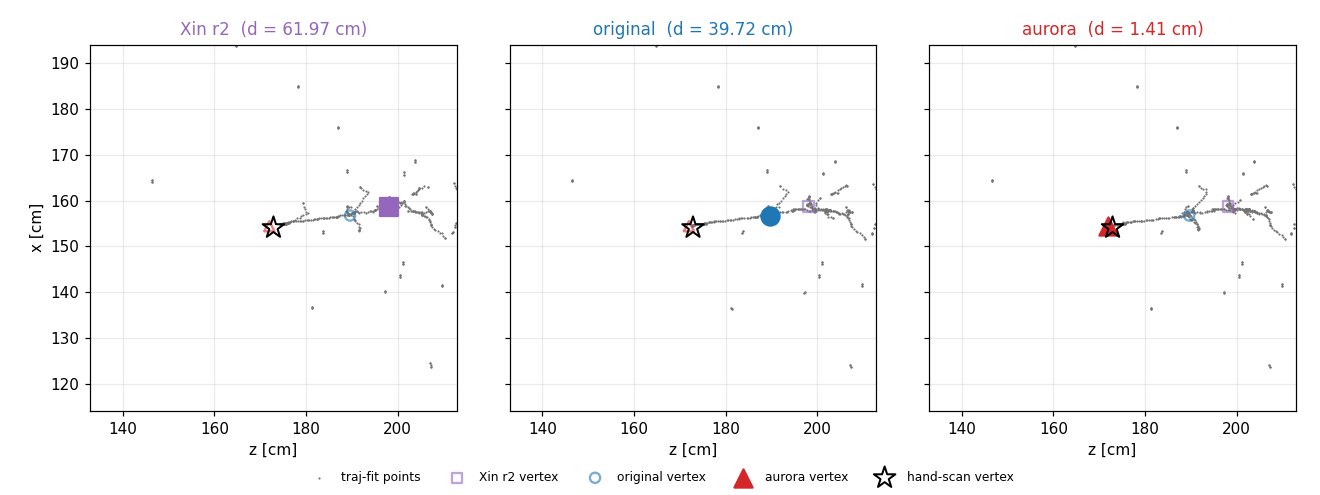
\includegraphics[width=0.92\linewidth]{figures/evt-18259-111412.png}\\[-2pt]
\scriptsize\raggedright
\textbf{Hand scan:} vertex (154.1, 80.0, 172.9) [scanner point], Xin r2 verdict: Not good, flavor: $\nu_e$CC; \textcolor{red}{selection changes}\\
\textit{Scan note: close to (x, y, z) = (154.1, 80.0, 172.9)}\\
\begin{tabular}{llcccc}
\toprule
method & & main vertex (x, y, z) cm & d to hand scan [cm] & $\nu_e$ / $\nu_\mu$ score & prediction \\
\midrule
Xin r2 & \href{https://www.phy.bnl.gov/twister/bee/set/9e2a1a1e-b637-4be5-99b7-f49bf8c04c57/event/12/}{Bee} & (158.7, 136.4, 198.1) & 61.97 & -- & -- \\
original & \href{https://www.phy.bnl.gov/twister/bee/set/89cdea53-c227-476c-8f67-0ae765f804b4/event/1/}{Bee} & (156.8, 115.9, 189.6) & 39.72 & -1.85 / 1.58 & $\nu_\mu$CC \\
aurora & \href{https://www.phy.bnl.gov/twister/bee/set/431dc57f-997d-4cff-88e1-4e33fd743ab8/event/1/}{Bee} & (154.4, 81.0, 172.0) & 1.41 & 8.08 / -1.07 & $\nu_e$ \\
\bottomrule
\end{tabular}
\end{frame}

\begin{frame}{nueCC-48: 18255/1/235435}
\vspace{-6pt}
\centering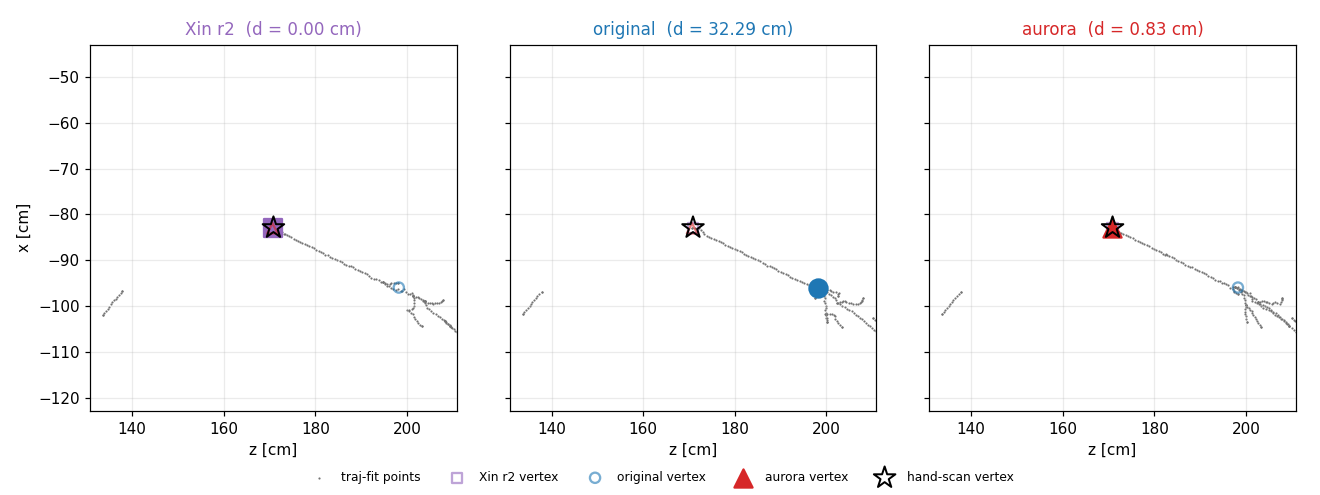
\includegraphics[width=0.92\linewidth]{figures/evt-18255-235435.png}\\[-2pt]
\scriptsize\raggedright
\textbf{Hand scan:} vertex (-82.9, 181.7, 170.9) [Xin r2 vertex (scan Good/OK)], Xin r2 verdict: Good, flavor: $\nu_e$CC; \textcolor{red}{selection changes}\\

\begin{tabular}{llcccc}
\toprule
method & & main vertex (x, y, z) cm & d to hand scan [cm] & $\nu_e$ / $\nu_\mu$ score & prediction \\
\midrule
Xin r2 & \href{https://www.phy.bnl.gov/twister/bee/set/9e2a1a1e-b637-4be5-99b7-f49bf8c04c57/event/25/}{Bee} & (-82.9, 181.7, 170.9) & \textbf{0.00} & -- & -- \\
original & \href{https://www.phy.bnl.gov/twister/bee/set/89cdea53-c227-476c-8f67-0ae765f804b4/event/2/}{Bee} & (-96.0, 192.8, 198.2) & 32.29 & -15.00 / 2.63 & $\nu_\mu$CC \\
aurora & \href{https://www.phy.bnl.gov/twister/bee/set/431dc57f-997d-4cff-88e1-4e33fd743ab8/event/2/}{Bee} & (-83.0, 182.5, 170.7) & \textbf{0.83} & 7.96 / 0.28 & $\nu_e$ \\
\bottomrule
\end{tabular}
\end{frame}

\begin{frame}{nueCC-48: 18255/1/163543}
\vspace{-6pt}
\centering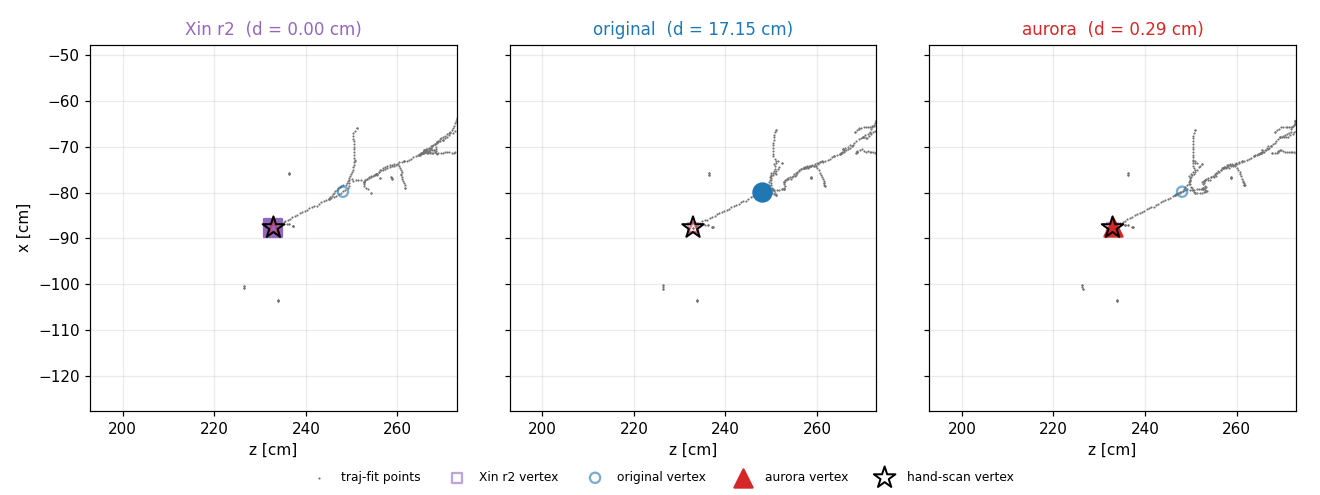
\includegraphics[width=0.92\linewidth]{figures/evt-18255-163543.png}\\[-2pt]
\scriptsize\raggedright
\textbf{Hand scan:} vertex (-87.7, -93.2, 232.9) [Xin r2 vertex (scan Good/OK)], Xin r2 verdict: Good, flavor: $\nu_e$CC; \textcolor{red}{selection changes}\\

\begin{tabular}{llcccc}
\toprule
method & & main vertex (x, y, z) cm & d to hand scan [cm] & $\nu_e$ / $\nu_\mu$ score & prediction \\
\midrule
Xin r2 & \href{https://www.phy.bnl.gov/twister/bee/set/9e2a1a1e-b637-4be5-99b7-f49bf8c04c57/event/17/}{Bee} & (-87.7, -93.2, 232.9) & \textbf{0.00} & -- & -- \\
original & \href{https://www.phy.bnl.gov/twister/bee/set/89cdea53-c227-476c-8f67-0ae765f804b4/event/3/}{Bee} & (-79.8, -94.6, 248.1) & 17.15 & 3.23 / -0.77 & other \\
aurora & \href{https://www.phy.bnl.gov/twister/bee/set/431dc57f-997d-4cff-88e1-4e33fd743ab8/event/3/}{Bee} & (-87.4, -93.4, 233.0) & \textbf{0.29} & 9.91 / -1.18 & $\nu_e$ \\
\bottomrule
\end{tabular}
\end{frame}

\begin{frame}{nueCC-48: 18255/1/268067}
\vspace{-6pt}
\centering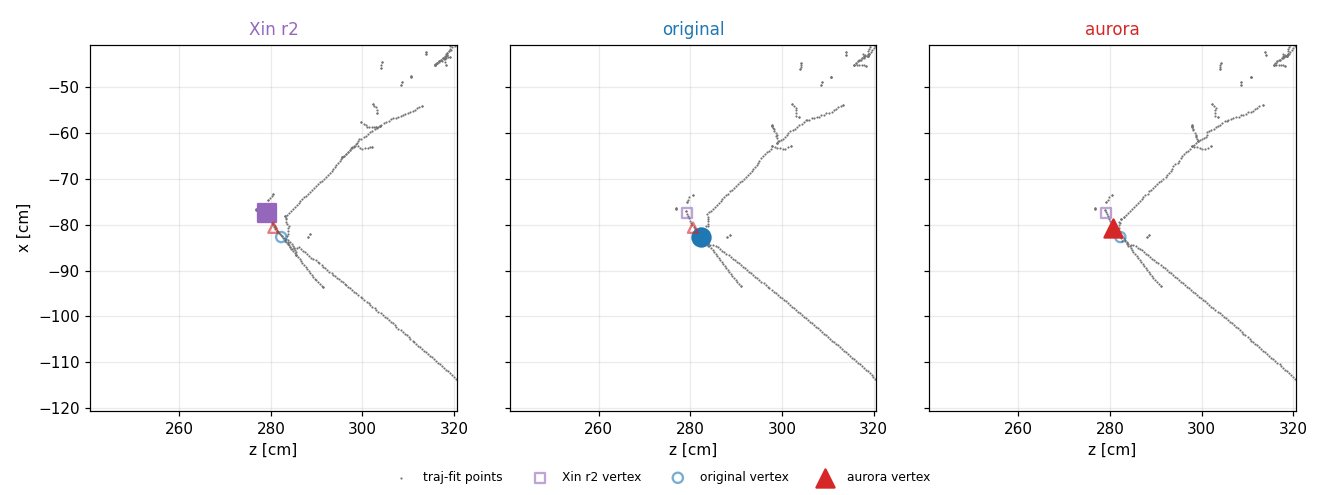
\includegraphics[width=0.92\linewidth]{figures/evt-18255-268067.png}\\[-2pt]
\scriptsize\raggedright
\textbf{Hand scan:} vertex -- [none], Xin r2 verdict: Not good, flavor: $\nu_e$CC; \textcolor{red}{selection changes}\\
\textit{Scan note: PR @ vertex needs improvements}\\
\begin{tabular}{llcccc}
\toprule
method & & main vertex (x, y, z) cm & d to hand scan [cm] & $\nu_e$ / $\nu_\mu$ score & prediction \\
\midrule
Xin r2 & \href{https://www.phy.bnl.gov/twister/bee/set/9e2a1a1e-b637-4be5-99b7-f49bf8c04c57/event/30/}{Bee} & (-77.5, -66.3, 279.2) & -- & -- & -- \\
original & \href{https://www.phy.bnl.gov/twister/bee/set/89cdea53-c227-476c-8f67-0ae765f804b4/event/4/}{Bee} & (-82.7, -63.5, 282.3) & -- & 8.34 / 0.51 & $\nu_e$ \\
aurora & \href{https://www.phy.bnl.gov/twister/bee/set/431dc57f-997d-4cff-88e1-4e33fd743ab8/event/4/}{Bee} & (-80.6, -64.7, 280.6) & -- & -15.00 / 0.52 & other \\
\bottomrule
\end{tabular}
\end{frame}

\begin{frame}{nueCC-48: 18255/1/360535}
\vspace{-6pt}
\centering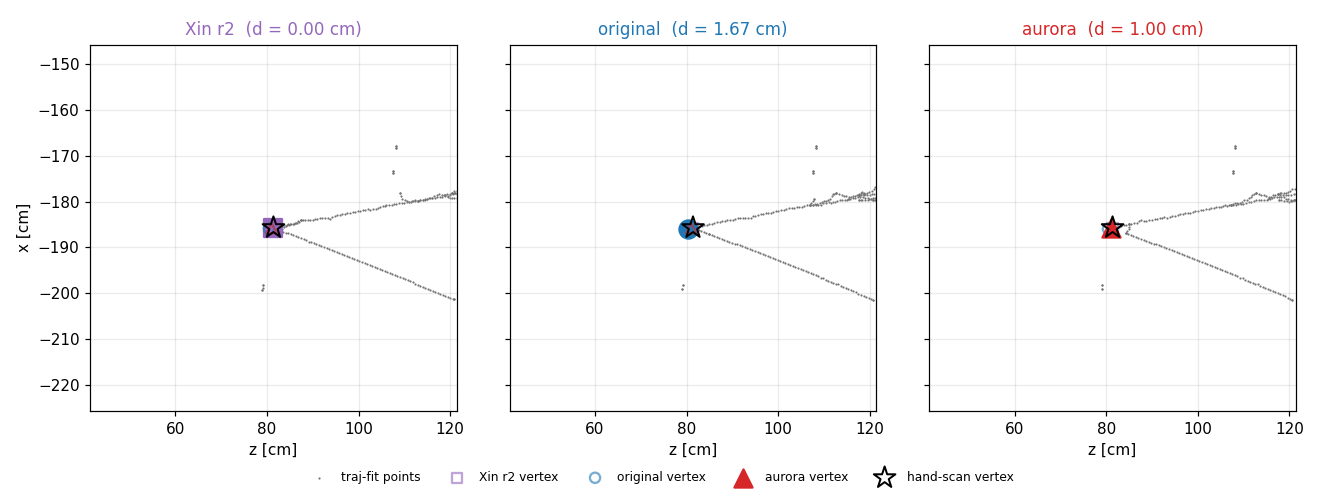
\includegraphics[width=0.92\linewidth]{figures/evt-18255-360535.png}\\[-2pt]
\scriptsize\raggedright
\textbf{Hand scan:} vertex (-185.7, -111.8, 81.4) [Xin r2 vertex (scan Good/OK)], Xin r2 verdict: Good, flavor: $\nu_e$CC; \textcolor{red}{selection changes}\\
\textit{Scan note: z OK}\\
\begin{tabular}{llcccc}
\toprule
method & & main vertex (x, y, z) cm & d to hand scan [cm] & $\nu_e$ / $\nu_\mu$ score & prediction \\
\midrule
Xin r2 & \href{https://www.phy.bnl.gov/twister/bee/set/9e2a1a1e-b637-4be5-99b7-f49bf8c04c57/event/36/}{Bee} & (-185.7, -111.8, 81.4) & \textbf{0.00} & -- & -- \\
original & \href{https://www.phy.bnl.gov/twister/bee/set/89cdea53-c227-476c-8f67-0ae765f804b4/event/6/}{Bee} & (-186.0, -110.5, 80.4) & 1.67 & 10.46 / -0.47 & $\nu_e$ \\
aurora & \href{https://www.phy.bnl.gov/twister/bee/set/431dc57f-997d-4cff-88e1-4e33fd743ab8/event/6/}{Bee} & (-185.8, -110.9, 81.0) & 1.00 & -15.00 / 0.09 & other \\
\bottomrule
\end{tabular}
\end{frame}

\begin{frame}{nueCC-48: 18255/1/268784}
\vspace{-6pt}
\centering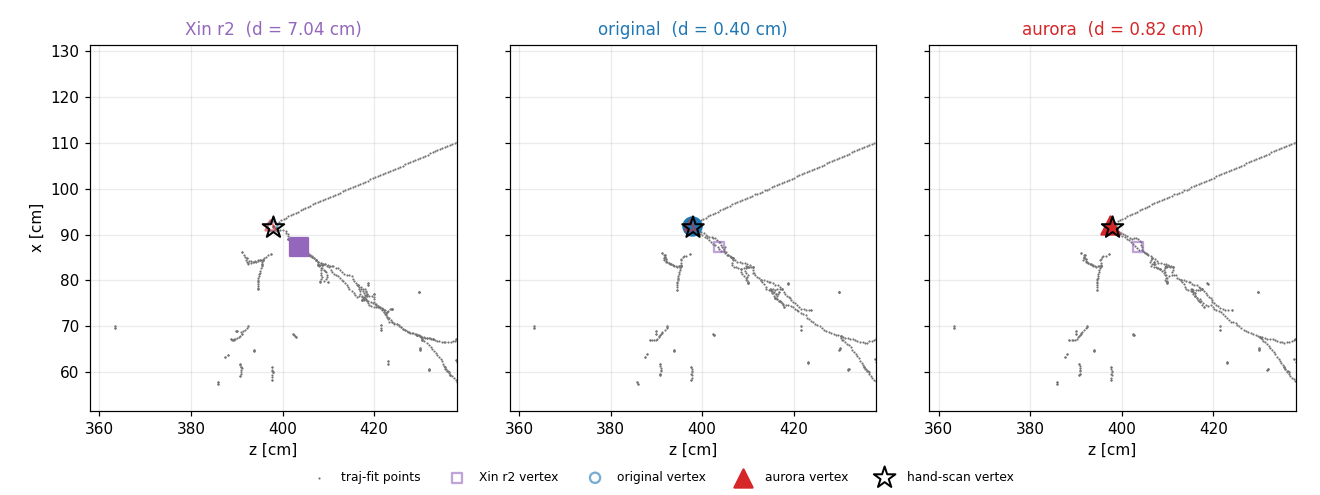
\includegraphics[width=0.92\linewidth]{figures/evt-18255-268784.png}\\[-2pt]
\scriptsize\raggedright
\textbf{Hand scan:} vertex (91.5, 19.5, 398.0) [scanner point], Xin r2 verdict: Not good, flavor: $\nu_e$CC; \textcolor{red}{selection changes}\\
\textit{Scan note: close to (x, y, z) = (91.5, 19.5, 398.0)}\\
\begin{tabular}{llcccc}
\toprule
method & & main vertex (x, y, z) cm & d to hand scan [cm] & $\nu_e$ / $\nu_\mu$ score & prediction \\
\midrule
Xin r2 & \href{https://www.phy.bnl.gov/twister/bee/set/9e2a1a1e-b637-4be5-99b7-f49bf8c04c57/event/31/}{Bee} & (87.3, 19.7, 403.6) & 7.04 & -- & -- \\
original & \href{https://www.phy.bnl.gov/twister/bee/set/89cdea53-c227-476c-8f67-0ae765f804b4/event/7/}{Bee} & (91.8, 19.6, 397.8) & \textbf{0.40} & 6.15 / 0.57 & other \\
aurora & \href{https://www.phy.bnl.gov/twister/bee/set/431dc57f-997d-4cff-88e1-4e33fd743ab8/event/7/}{Bee} & (92.0, 19.6, 397.4) & \textbf{0.82} & 8.39 / 0.08 & $\nu_e$ \\
\bottomrule
\end{tabular}
\end{frame}

\begin{frame}{nueCC-48: 18255/1/168596}
\vspace{-6pt}
\centering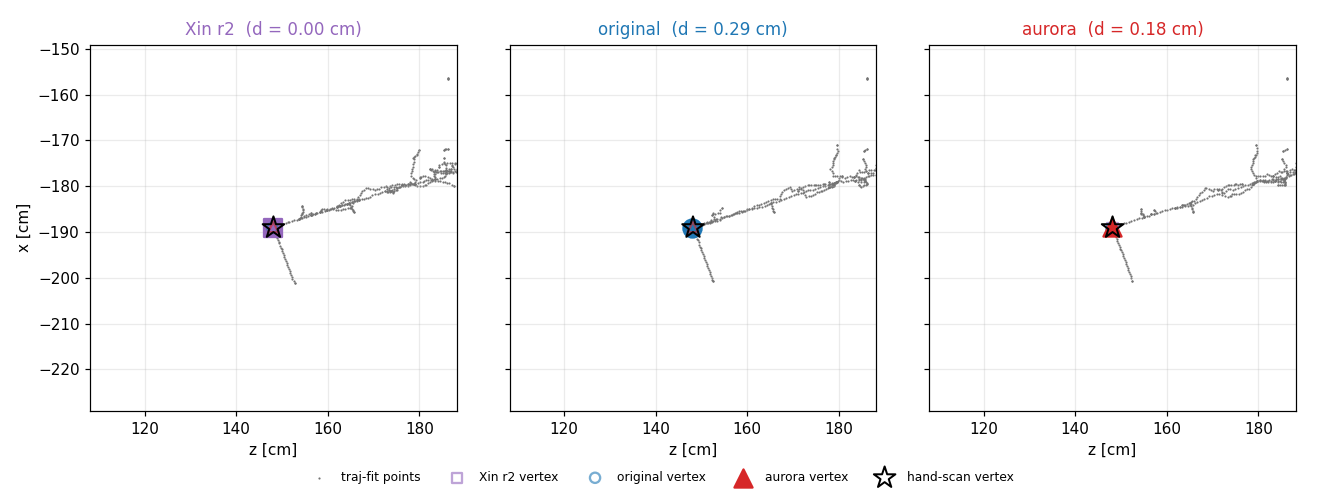
\includegraphics[width=0.92\linewidth]{figures/evt-18255-168596.png}\\[-2pt]
\scriptsize\raggedright
\textbf{Hand scan:} vertex (-189.0, 25.5, 148.2) [Xin r2 vertex (scan Good/OK)], Xin r2 verdict: Good, flavor: $\nu_e$CC; \textcolor{red}{selection changes}\\

\begin{tabular}{llcccc}
\toprule
method & & main vertex (x, y, z) cm & d to hand scan [cm] & $\nu_e$ / $\nu_\mu$ score & prediction \\
\midrule
Xin r2 & \href{https://www.phy.bnl.gov/twister/bee/set/9e2a1a1e-b637-4be5-99b7-f49bf8c04c57/event/18/}{Bee} & (-189.0, 25.5, 148.2) & \textbf{0.00} & -- & -- \\
original & \href{https://www.phy.bnl.gov/twister/bee/set/89cdea53-c227-476c-8f67-0ae765f804b4/event/8/}{Bee} & (-189.1, 25.6, 147.9) & \textbf{0.29} & -0.27 / 0.34 & other \\
aurora & \href{https://www.phy.bnl.gov/twister/bee/set/431dc57f-997d-4cff-88e1-4e33fd743ab8/event/8/}{Bee} & (-188.9, 25.5, 148.1) & \textbf{0.18} & 10.90 / 0.25 & $\nu_e$ \\
\bottomrule
\end{tabular}
\end{frame}

\begin{frame}{nueCC-48: 18259/1/116962}
\vspace{-6pt}
\centering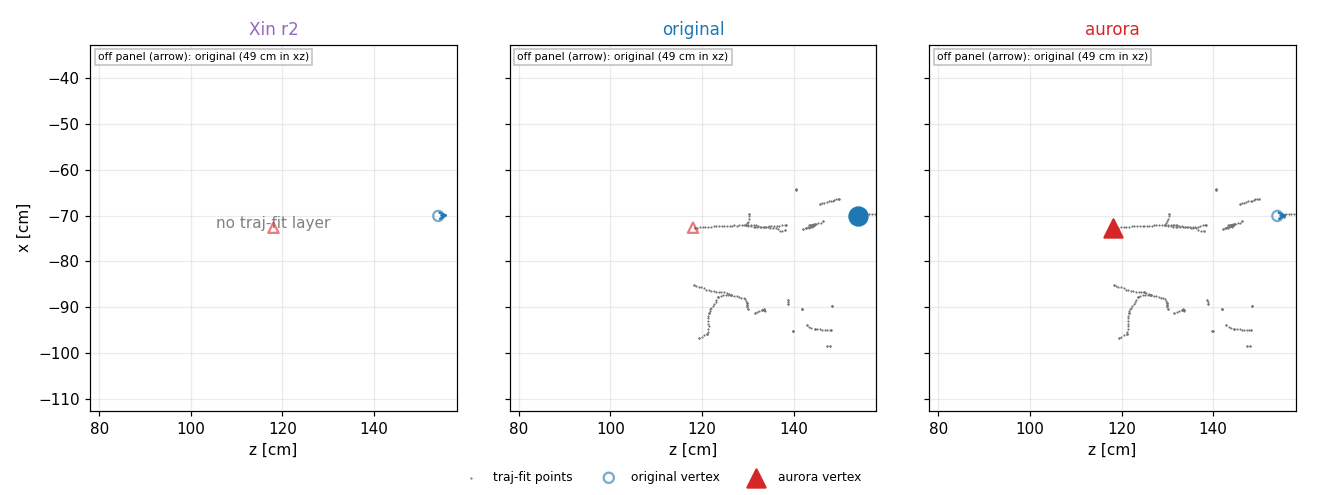
\includegraphics[width=0.92\linewidth]{figures/evt-18259-116962.png}\\[-2pt]
\scriptsize\raggedright
\textbf{Hand scan:} vertex -- [none], Xin r2 verdict: --, flavor: $\nu_e$CC; not in the scan sheet\\

\begin{tabular}{llcccc}
\toprule
method & & main vertex (x, y, z) cm & d to hand scan [cm] & $\nu_e$ / $\nu_\mu$ score & prediction \\
\midrule
Xin r2 & -- & -- & -- & -- & -- \\
original & \href{https://www.phy.bnl.gov/twister/bee/set/89cdea53-c227-476c-8f67-0ae765f804b4/event/9/}{Bee} & (-69.2, -81.3, 166.5) & -- & -4.82 / 0.15 & other \\
aurora & \href{https://www.phy.bnl.gov/twister/bee/set/431dc57f-997d-4cff-88e1-4e33fd743ab8/event/9/}{Bee} & (-72.6, -79.3, 118.0) & -- & -15.00 / -0.04 & other \\
\bottomrule
\end{tabular}
\end{frame}

\begin{frame}{nueCC-48: 18255/1/469665}
\vspace{-6pt}
\centering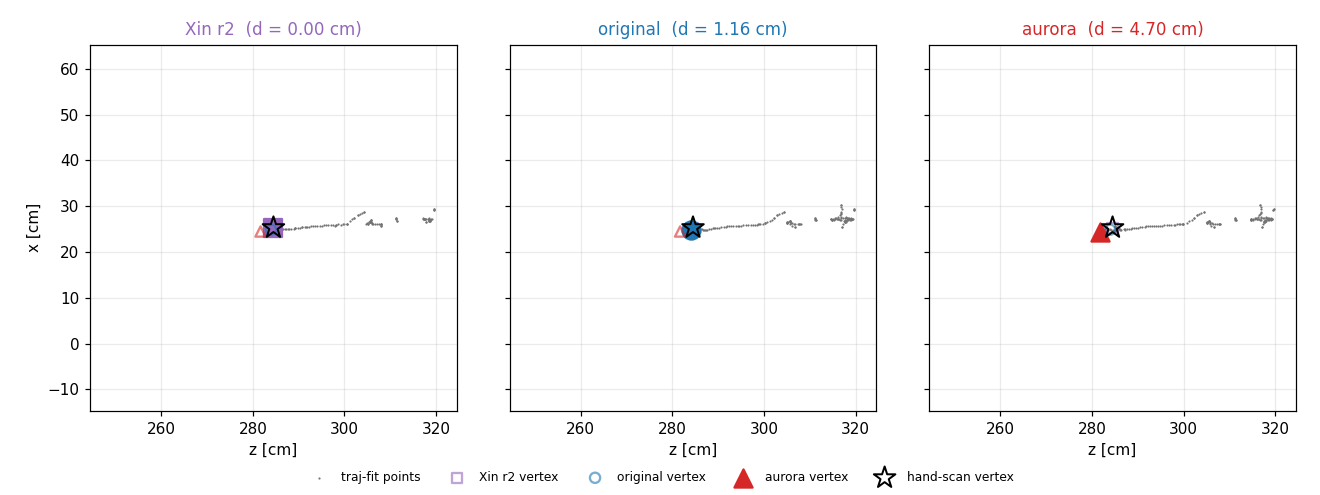
\includegraphics[width=0.92\linewidth]{figures/evt-18255-469665.png}\\[-2pt]
\scriptsize\raggedright
\textbf{Hand scan:} vertex (25.3, 61.6, 284.5) [Xin r2 vertex (scan Good/OK)], Xin r2 verdict: Good, flavor: $\nu_e$CC\\
\textit{Scan note: electron trunk ided as muon}\\
\begin{tabular}{llcccc}
\toprule
method & & main vertex (x, y, z) cm & d to hand scan [cm] & $\nu_e$ / $\nu_\mu$ score & prediction \\
\midrule
Xin r2 & \href{https://www.phy.bnl.gov/twister/bee/set/9e2a1a1e-b637-4be5-99b7-f49bf8c04c57/event/45/}{Bee} & (25.3, 61.6, 284.5) & \textbf{0.00} & -- & -- \\
original & \href{https://www.phy.bnl.gov/twister/bee/set/89cdea53-c227-476c-8f67-0ae765f804b4/event/14/}{Bee} & (24.9, 62.5, 284.0) & 1.16 & 3.81 / -0.49 & other \\
aurora & \href{https://www.phy.bnl.gov/twister/bee/set/431dc57f-997d-4cff-88e1-4e33fd743ab8/event/14/}{Bee} & (24.5, 65.2, 281.7) & 4.70 & 2.96 / -0.13 & other \\
\bottomrule
\end{tabular}
\end{frame}

\begin{frame}{nueCC-48: 18255/1/196649}
\vspace{-6pt}
\centering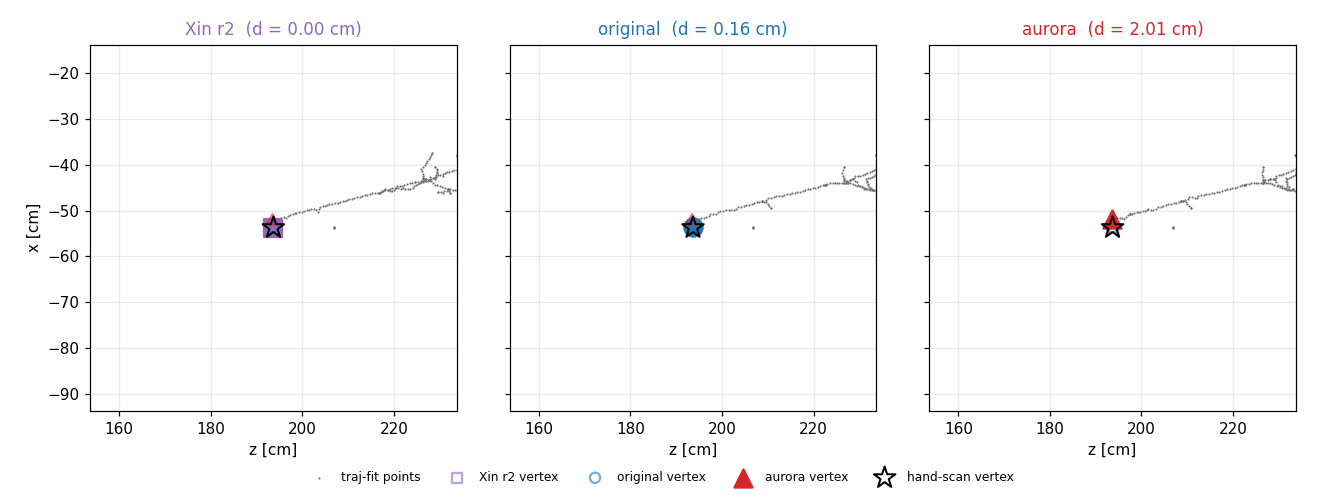
\includegraphics[width=0.92\linewidth]{figures/evt-18255-196649.png}\\[-2pt]
\scriptsize\raggedright
\textbf{Hand scan:} vertex (-53.7, -21.5, 193.7) [Xin r2 vertex (scan Good/OK)], Xin r2 verdict: OK, flavor: $\nu_e$CC\\
\textit{Scan note: missing a vertex particle?}\\
\begin{tabular}{llcccc}
\toprule
method & & main vertex (x, y, z) cm & d to hand scan [cm] & $\nu_e$ / $\nu_\mu$ score & prediction \\
\midrule
Xin r2 & \href{https://www.phy.bnl.gov/twister/bee/set/9e2a1a1e-b637-4be5-99b7-f49bf8c04c57/event/21/}{Bee} & (-53.7, -21.5, 193.7) & \textbf{0.00} & -- & -- \\
original & \href{https://www.phy.bnl.gov/twister/bee/set/89cdea53-c227-476c-8f67-0ae765f804b4/event/18/}{Bee} & (-53.6, -21.5, 193.7) & \textbf{0.16} & 7.97 / -0.54 & $\nu_e$ \\
aurora & \href{https://www.phy.bnl.gov/twister/bee/set/431dc57f-997d-4cff-88e1-4e33fd743ab8/event/18/}{Bee} & (-51.9, -20.7, 193.5) & 2.01 & 12.45 / -0.41 & $\nu_e$ \\
\bottomrule
\end{tabular}
\end{frame}

\begin{frame}{nueCC-48: 18304/1/38856}
\vspace{-6pt}
\centering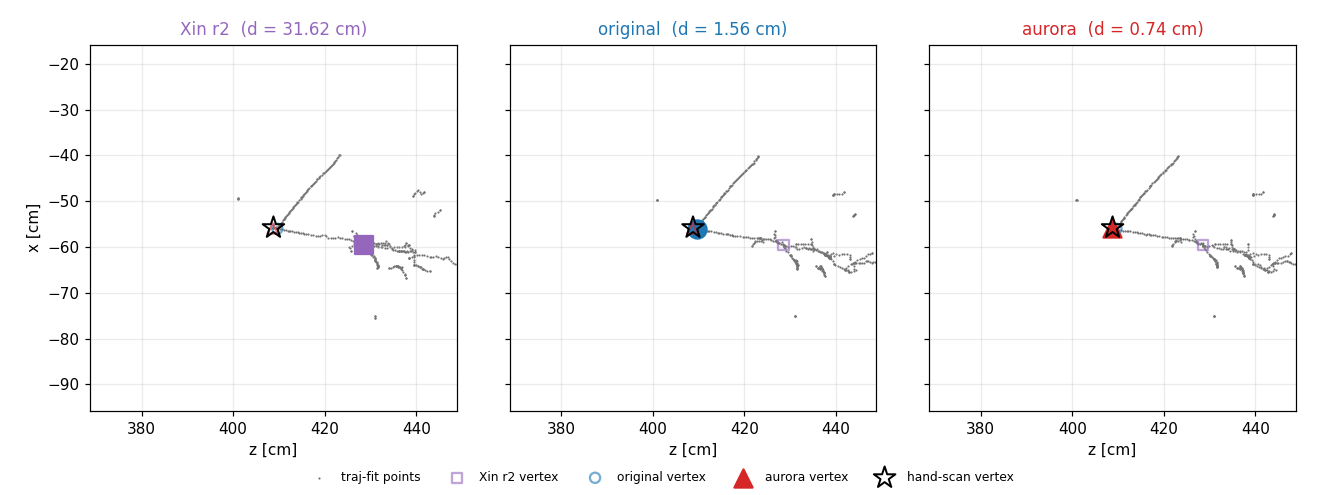
\includegraphics[width=0.92\linewidth]{figures/evt-18304-38856.png}\\[-2pt]
\scriptsize\raggedright
\textbf{Hand scan:} vertex (-55.8, -78.8, 408.8) [scanner point], Xin r2 verdict: Not OK, flavor: $\nu_e$CC\\
\textit{Scan note: close to (x, y, z) = (-55.8, -78.8, 408.8)}\\
\begin{tabular}{llcccc}
\toprule
method & & main vertex (x, y, z) cm & d to hand scan [cm] & $\nu_e$ / $\nu_\mu$ score & prediction \\
\midrule
Xin r2 & \href{https://www.phy.bnl.gov/twister/bee/set/9e2a1a1e-b637-4be5-99b7-f49bf8c04c57/event/3/}{Bee} & (-59.6, -54.4, 428.6) & 31.62 & -- & -- \\
original & \href{https://www.phy.bnl.gov/twister/bee/set/89cdea53-c227-476c-8f67-0ae765f804b4/event/19/}{Bee} & (-56.0, -77.5, 409.6) & 1.56 & 13.69 / -0.90 & $\nu_e$ \\
aurora & \href{https://www.phy.bnl.gov/twister/bee/set/431dc57f-997d-4cff-88e1-4e33fd743ab8/event/19/}{Bee} & (-56.0, -78.1, 408.6) & \textbf{0.74} & 14.21 / 0.26 & $\nu_e$ \\
\bottomrule
\end{tabular}
\end{frame}

\begin{frame}{nueCC-48: 18255/1/69314}
\vspace{-6pt}
\centering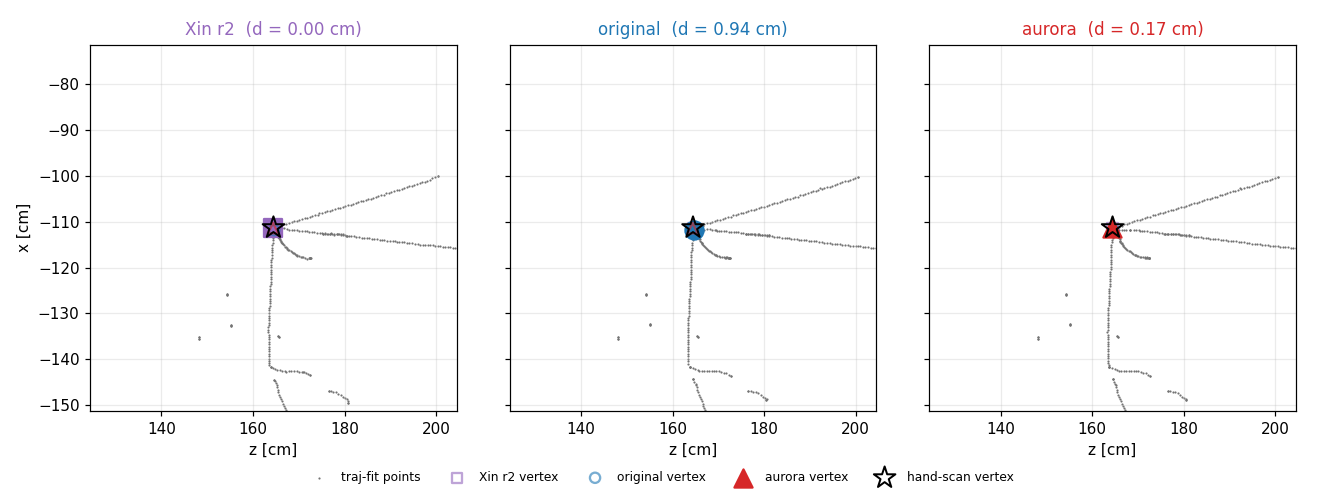
\includegraphics[width=0.92\linewidth]{figures/evt-18255-69314.png}\\[-2pt]
\scriptsize\raggedright
\textbf{Hand scan:} vertex (-111.3, -17.8, 164.5) [Xin r2 vertex (scan Good/OK)], Xin r2 verdict: Good, flavor: $\nu_e$CC\\
\textit{Scan note: missing pi\textasciicircum{}+ --$>$ pi0?}\\
\begin{tabular}{llcccc}
\toprule
method & & main vertex (x, y, z) cm & d to hand scan [cm] & $\nu_e$ / $\nu_\mu$ score & prediction \\
\midrule
Xin r2 & \href{https://www.phy.bnl.gov/twister/bee/set/9e2a1a1e-b637-4be5-99b7-f49bf8c04c57/event/8/}{Bee} & (-111.3, -17.8, 164.5) & \textbf{0.00} & -- & -- \\
original & \href{https://www.phy.bnl.gov/twister/bee/set/89cdea53-c227-476c-8f67-0ae765f804b4/event/20/}{Bee} & (-111.8, -18.5, 164.6) & \textbf{0.94} & -15.00 / 2.96 & $\nu_\mu$CC \\
aurora & \href{https://www.phy.bnl.gov/twister/bee/set/431dc57f-997d-4cff-88e1-4e33fd743ab8/event/20/}{Bee} & (-111.4, -17.9, 164.4) & \textbf{0.17} & -9.77 / 2.13 & $\nu_\mu$CC \\
\bottomrule
\end{tabular}
\end{frame}

\begin{frame}{nueCC-48: 18255/1/122660}
\vspace{-6pt}
\centering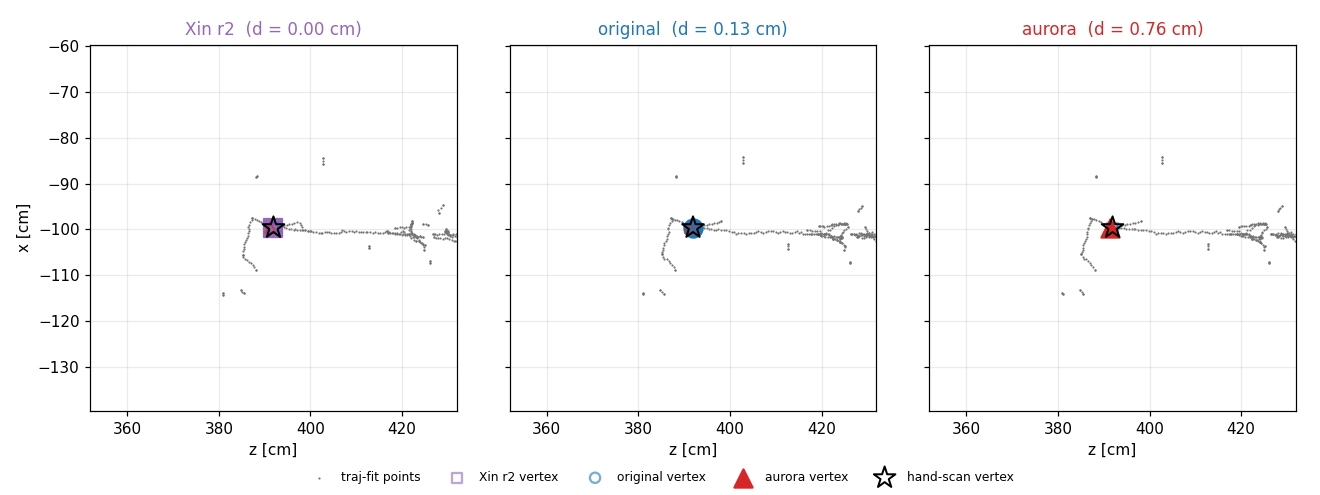
\includegraphics[width=0.92\linewidth]{figures/evt-18255-122660.png}\\[-2pt]
\scriptsize\raggedright
\textbf{Hand scan:} vertex (-99.6, -76.7, 391.9) [Xin r2 vertex (scan Good/OK)], Xin r2 verdict: Good, flavor: $\nu_e$CC\\

\begin{tabular}{llcccc}
\toprule
method & & main vertex (x, y, z) cm & d to hand scan [cm] & $\nu_e$ / $\nu_\mu$ score & prediction \\
\midrule
Xin r2 & \href{https://www.phy.bnl.gov/twister/bee/set/9e2a1a1e-b637-4be5-99b7-f49bf8c04c57/event/13/}{Bee} & (-99.6, -76.7, 391.9) & \textbf{0.00} & -- & -- \\
original & \href{https://www.phy.bnl.gov/twister/bee/set/89cdea53-c227-476c-8f67-0ae765f804b4/event/25/}{Bee} & (-99.6, -76.8, 391.9) & \textbf{0.13} & 10.36 / 0.53 & $\nu_e$ \\
aurora & \href{https://www.phy.bnl.gov/twister/bee/set/431dc57f-997d-4cff-88e1-4e33fd743ab8/event/25/}{Bee} & (-99.6, -77.1, 391.3) & \textbf{0.76} & 10.65 / 0.47 & $\nu_e$ \\
\bottomrule
\end{tabular}
\end{frame}

\begin{frame}{nueCC-48: 18255/1/90055}
\vspace{-6pt}
\centering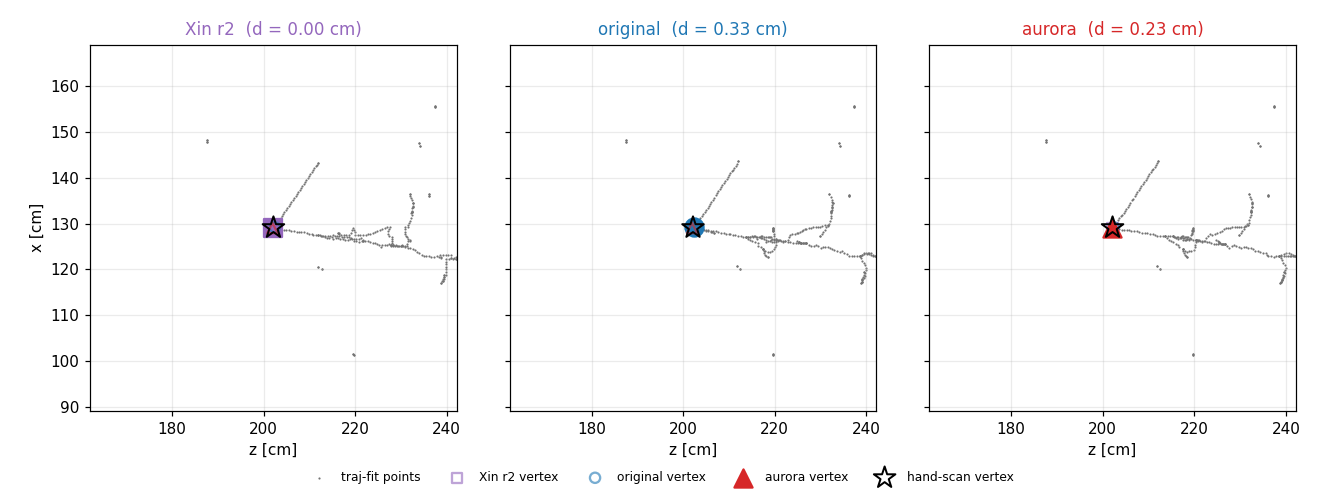
\includegraphics[width=0.92\linewidth]{figures/evt-18255-90055.png}\\[-2pt]
\scriptsize\raggedright
\textbf{Hand scan:} vertex (129.1, 24.9, 202.1) [Xin r2 vertex (scan Good/OK)], Xin r2 verdict: Good, flavor: $\nu_e$CC\\
\textit{Scan note: EM shower trunk mis-ided as proton}\\
\begin{tabular}{llcccc}
\toprule
method & & main vertex (x, y, z) cm & d to hand scan [cm] & $\nu_e$ / $\nu_\mu$ score & prediction \\
\midrule
Xin r2 & \href{https://www.phy.bnl.gov/twister/bee/set/9e2a1a1e-b637-4be5-99b7-f49bf8c04c57/event/11/}{Bee} & (129.1, 24.9, 202.1) & \textbf{0.00} & -- & -- \\
original & \href{https://www.phy.bnl.gov/twister/bee/set/89cdea53-c227-476c-8f67-0ae765f804b4/event/26/}{Bee} & (129.2, 24.8, 202.4) & \textbf{0.33} & 11.27 / -0.73 & $\nu_e$ \\
aurora & \href{https://www.phy.bnl.gov/twister/bee/set/431dc57f-997d-4cff-88e1-4e33fd743ab8/event/26/}{Bee} & (129.0, 24.9, 201.9) & \textbf{0.23} & 10.95 / -0.76 & $\nu_e$ \\
\bottomrule
\end{tabular}
\end{frame}

\begin{frame}{nueCC-48: 18255/1/437699}
\vspace{-6pt}
\centering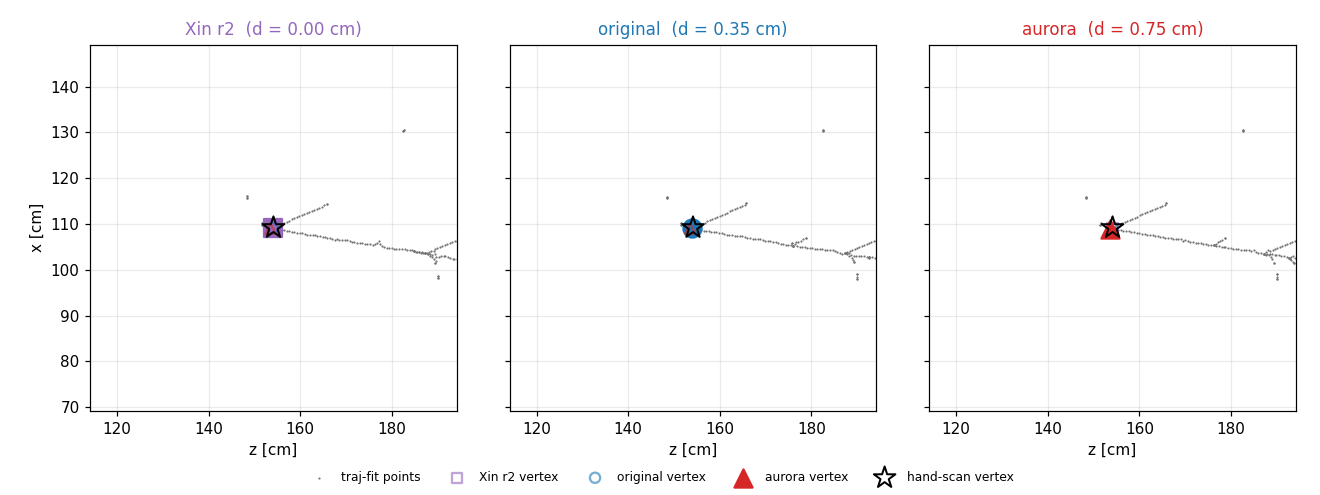
\includegraphics[width=0.92\linewidth]{figures/evt-18255-437699.png}\\[-2pt]
\scriptsize\raggedright
\textbf{Hand scan:} vertex (109.2, -148.9, 154.1) [Xin r2 vertex (scan Good/OK)], Xin r2 verdict: Good, flavor: $\nu_e$CC\\

\begin{tabular}{llcccc}
\toprule
method & & main vertex (x, y, z) cm & d to hand scan [cm] & $\nu_e$ / $\nu_\mu$ score & prediction \\
\midrule
Xin r2 & \href{https://www.phy.bnl.gov/twister/bee/set/9e2a1a1e-b637-4be5-99b7-f49bf8c04c57/event/42/}{Bee} & (109.2, -148.9, 154.1) & \textbf{0.00} & -- & -- \\
original & \href{https://www.phy.bnl.gov/twister/bee/set/89cdea53-c227-476c-8f67-0ae765f804b4/event/27/}{Bee} & (109.1, -149.3, 154.0) & \textbf{0.35} & 8.51 / -0.69 & $\nu_e$ \\
aurora & \href{https://www.phy.bnl.gov/twister/bee/set/431dc57f-997d-4cff-88e1-4e33fd743ab8/event/27/}{Bee} & (109.0, -149.3, 153.5) & \textbf{0.75} & 9.64 / -0.97 & $\nu_e$ \\
\bottomrule
\end{tabular}
\end{frame}

\begin{frame}{nueCC-48: 18264/1/137238}
\vspace{-6pt}
\centering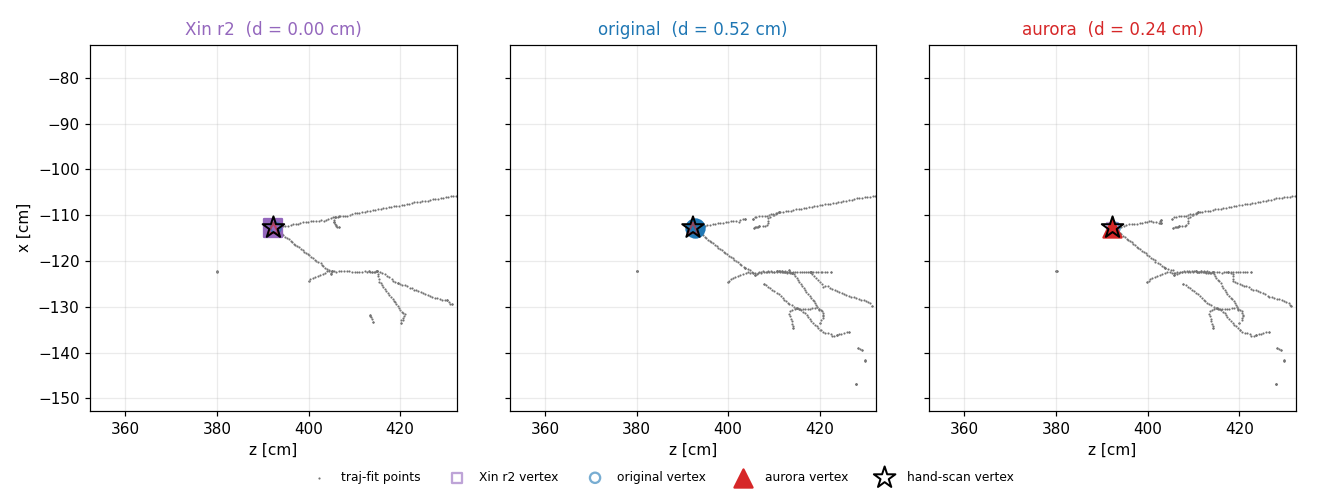
\includegraphics[width=0.92\linewidth]{figures/evt-18264-137238.png}\\[-2pt]
\scriptsize\raggedright
\textbf{Hand scan:} vertex (-112.7, 30.4, 392.3) [Xin r2 vertex (scan Good/OK)], Xin r2 verdict: Good, flavor: $\nu_e$CC\\
\textit{Scan note: missing some trajectories??? fixed}\\
\begin{tabular}{llcccc}
\toprule
method & & main vertex (x, y, z) cm & d to hand scan [cm] & $\nu_e$ / $\nu_\mu$ score & prediction \\
\midrule
Xin r2 & \href{https://www.phy.bnl.gov/twister/bee/set/9e2a1a1e-b637-4be5-99b7-f49bf8c04c57/event/15/}{Bee} & (-112.7, 30.4, 392.3) & \textbf{0.00} & -- & -- \\
original & \href{https://www.phy.bnl.gov/twister/bee/set/89cdea53-c227-476c-8f67-0ae765f804b4/event/28/}{Bee} & (-112.8, 30.2, 392.8) & \textbf{0.52} & -15.00 / 1.65 & $\nu_\mu$CC \\
aurora & \href{https://www.phy.bnl.gov/twister/bee/set/431dc57f-997d-4cff-88e1-4e33fd743ab8/event/28/}{Bee} & (-112.8, 30.2, 392.3) & \textbf{0.24} & -15.00 / 2.02 & $\nu_\mu$CC \\
\bottomrule
\end{tabular}
\end{frame}

\begin{frame}{nueCC-48: 18259/1/42280}
\vspace{-6pt}
\centering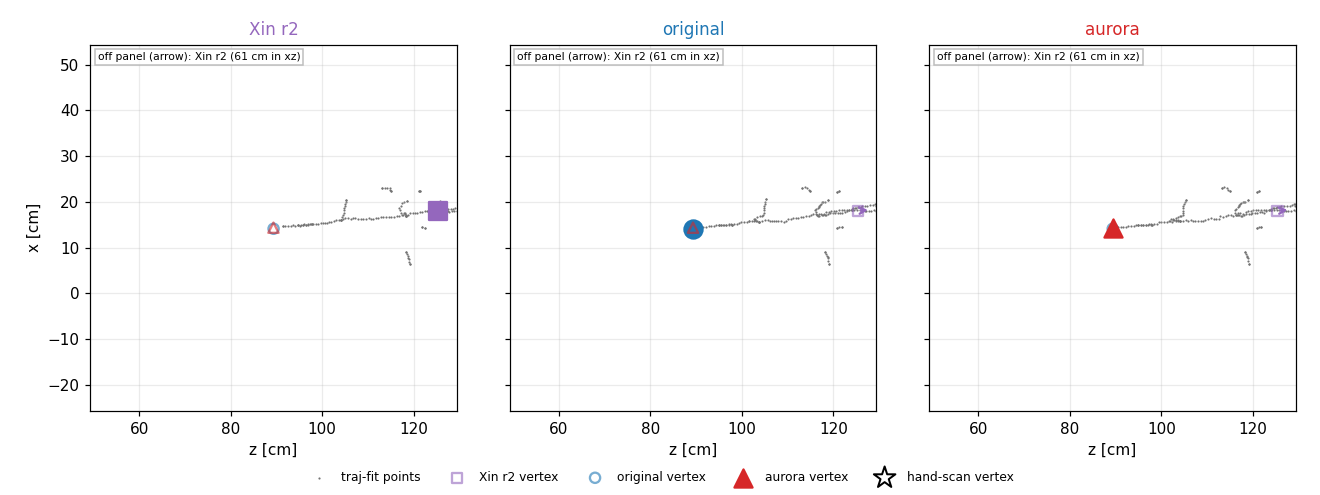
\includegraphics[width=0.92\linewidth]{figures/evt-18259-42280.png}\\[-2pt]
\scriptsize\raggedright
\textbf{Hand scan:} vertex (20.6, 4.4, 150.2) [Xin r2 vertex (scan Good/OK)], Xin r2 verdict: Good, flavor: $\nu_e$CC; \textcolor{orange!80!black}{our candidate $\ne$ scanned interaction}\\
\textit{Scan note: close to (x, y, z) = (13.7, -10.0, 89.4) missing vertex proton}\\
\begin{tabular}{llcccc}
\toprule
method & & main vertex (x, y, z) cm & d to hand scan [cm] & $\nu_e$ / $\nu_\mu$ score & prediction \\
\midrule
Xin r2 & \href{https://www.phy.bnl.gov/twister/bee/set/9e2a1a1e-b637-4be5-99b7-f49bf8c04c57/event/4/}{Bee} & (20.6, 4.4, 150.2) & -- & -- & -- \\
original & \href{https://www.phy.bnl.gov/twister/bee/set/89cdea53-c227-476c-8f67-0ae765f804b4/event/29/}{Bee} & (14.1, -10.2, 89.4) & -- & 12.72 / -1.73 & $\nu_e$ \\
aurora & \href{https://www.phy.bnl.gov/twister/bee/set/431dc57f-997d-4cff-88e1-4e33fd743ab8/event/29/}{Bee} & (14.4, -9.8, 89.3) & -- & 8.88 / -0.71 & $\nu_e$ \\
\bottomrule
\end{tabular}
\end{frame}

\begin{frame}{nueCC-48: 18342/1/30504}
\vspace{-6pt}
\centering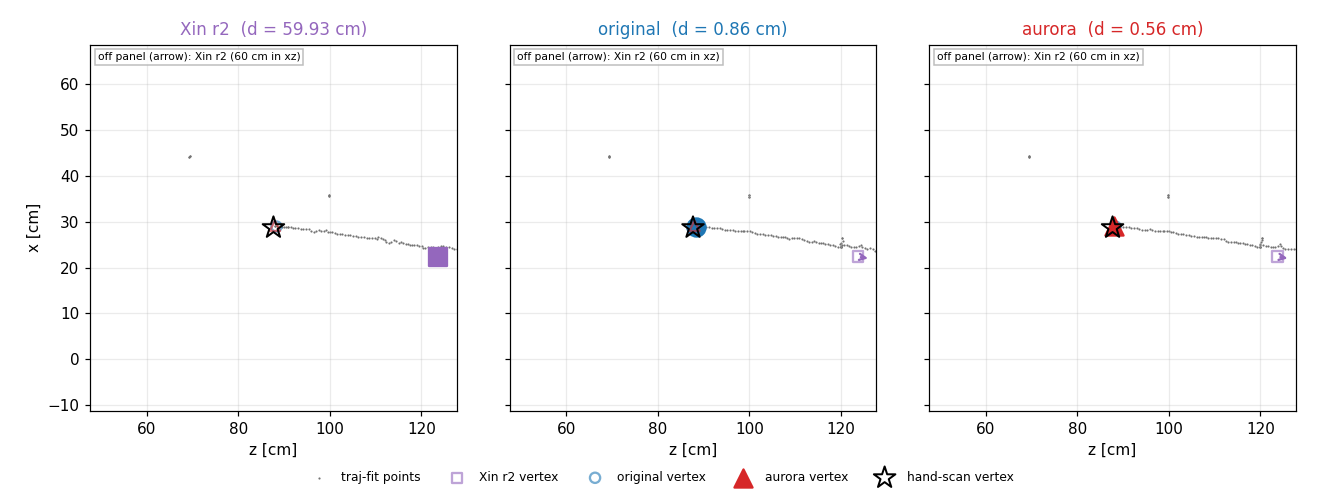
\includegraphics[width=0.92\linewidth]{figures/evt-18342-30504.png}\\[-2pt]
\scriptsize\raggedright
\textbf{Hand scan:} vertex (28.7, -50.7, 87.7) [scanner point], Xin r2 verdict: Not OK, flavor: $\nu_e$CC\\
\textit{Scan note: @ (x, y, z) = (28.7, -50.7, 87.7)}\\
\begin{tabular}{llcccc}
\toprule
method & & main vertex (x, y, z) cm & d to hand scan [cm] & $\nu_e$ / $\nu_\mu$ score & prediction \\
\midrule
Xin r2 & \href{https://www.phy.bnl.gov/twister/bee/set/9e2a1a1e-b637-4be5-99b7-f49bf8c04c57/event/2/}{Bee} & (18.4, -49.0, 146.7) & 59.93 & -- & -- \\
original & \href{https://www.phy.bnl.gov/twister/bee/set/89cdea53-c227-476c-8f67-0ae765f804b4/event/30/}{Bee} & (28.9, -51.2, 88.4) & \textbf{0.86} & 9.21 / -0.45 & $\nu_e$ \\
aurora & \href{https://www.phy.bnl.gov/twister/bee/set/431dc57f-997d-4cff-88e1-4e33fd743ab8/event/30/}{Bee} & (29.1, -50.9, 88.0) & \textbf{0.56} & 11.61 / -0.30 & $\nu_e$ \\
\bottomrule
\end{tabular}
\end{frame}

\begin{frame}{nueCC-48: 18255/1/269774}
\vspace{-6pt}
\centering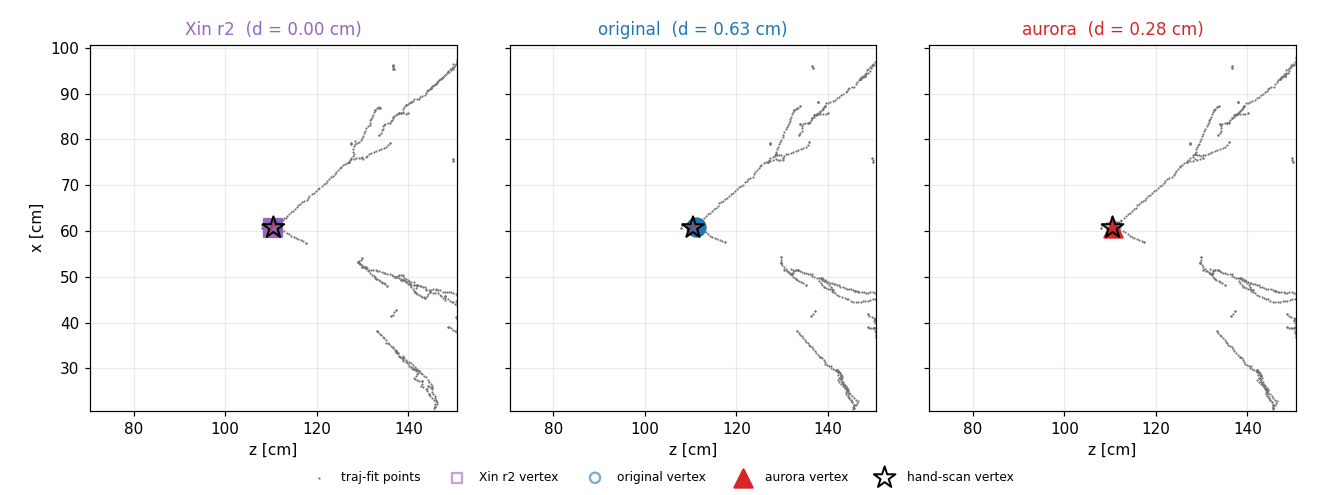
\includegraphics[width=0.92\linewidth]{figures/evt-18255-269774.png}\\[-2pt]
\scriptsize\raggedright
\textbf{Hand scan:} vertex (60.7, -10.2, 110.5) [Xin r2 vertex (scan Good/OK)], Xin r2 verdict: Good, flavor: $\nu_e$CC\\
\textit{Scan note: Multiple pi0 correct?}\\
\begin{tabular}{llcccc}
\toprule
method & & main vertex (x, y, z) cm & d to hand scan [cm] & $\nu_e$ / $\nu_\mu$ score & prediction \\
\midrule
Xin r2 & \href{https://www.phy.bnl.gov/twister/bee/set/9e2a1a1e-b637-4be5-99b7-f49bf8c04c57/event/32/}{Bee} & (60.7, -10.2, 110.5) & \textbf{0.00} & -- & -- \\
original & \href{https://www.phy.bnl.gov/twister/bee/set/89cdea53-c227-476c-8f67-0ae765f804b4/event/31/}{Bee} & (60.9, -10.3, 111.2) & \textbf{0.63} & 10.83 / -1.06 & $\nu_e$ \\
aurora & \href{https://www.phy.bnl.gov/twister/bee/set/431dc57f-997d-4cff-88e1-4e33fd743ab8/event/31/}{Bee} & (60.7, -10.4, 110.7) & \textbf{0.28} & 11.42 / -0.83 & $\nu_e$ \\
\bottomrule
\end{tabular}
\end{frame}

\begin{frame}{nueCC-48: 18259/1/52672}
\vspace{-6pt}
\centering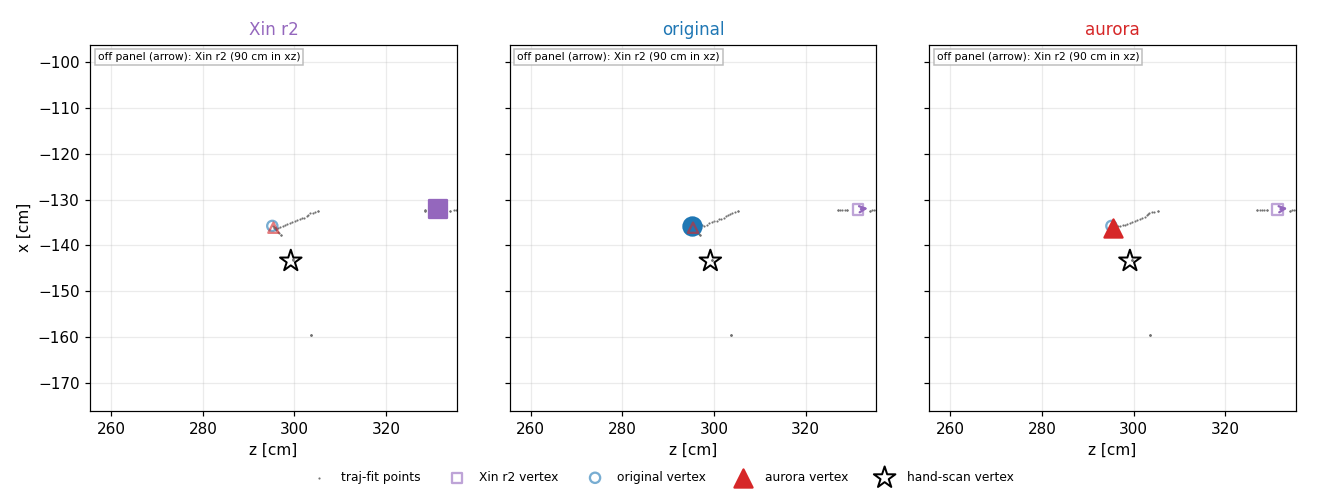
\includegraphics[width=0.92\linewidth]{figures/evt-18259-52672.png}\\[-2pt]
\scriptsize\raggedright
\textbf{Hand scan:} vertex (-143.4, 77.7, 299.2) [scanner point], Xin r2 verdict: Not OK, flavor: $\nu_e$CC; \textcolor{orange!80!black}{our candidate $\ne$ scanned interaction}\\
\textit{Scan note: close to (x, y, z) = (-143.4, 77.7, 299.2)}\\
\begin{tabular}{llcccc}
\toprule
method & & main vertex (x, y, z) cm & d to hand scan [cm] & $\nu_e$ / $\nu_\mu$ score & prediction \\
\midrule
Xin r2 & \href{https://www.phy.bnl.gov/twister/bee/set/9e2a1a1e-b637-4be5-99b7-f49bf8c04c57/event/6/}{Bee} & (-126.2, 85.4, 385.1) & -- & -- & -- \\
original & \href{https://www.phy.bnl.gov/twister/bee/set/89cdea53-c227-476c-8f67-0ae765f804b4/event/32/}{Bee} & (-135.7, 66.7, 295.2) & -- & 13.28 / -0.10 & $\nu_e$ \\
aurora & \href{https://www.phy.bnl.gov/twister/bee/set/431dc57f-997d-4cff-88e1-4e33fd743ab8/event/32/}{Bee} & (-136.1, 66.7, 295.4) & -- & 11.17 / -0.09 & $\nu_e$ \\
\bottomrule
\end{tabular}
\end{frame}

\begin{frame}{nueCC-48: 18255/1/46363}
\vspace{-6pt}
\centering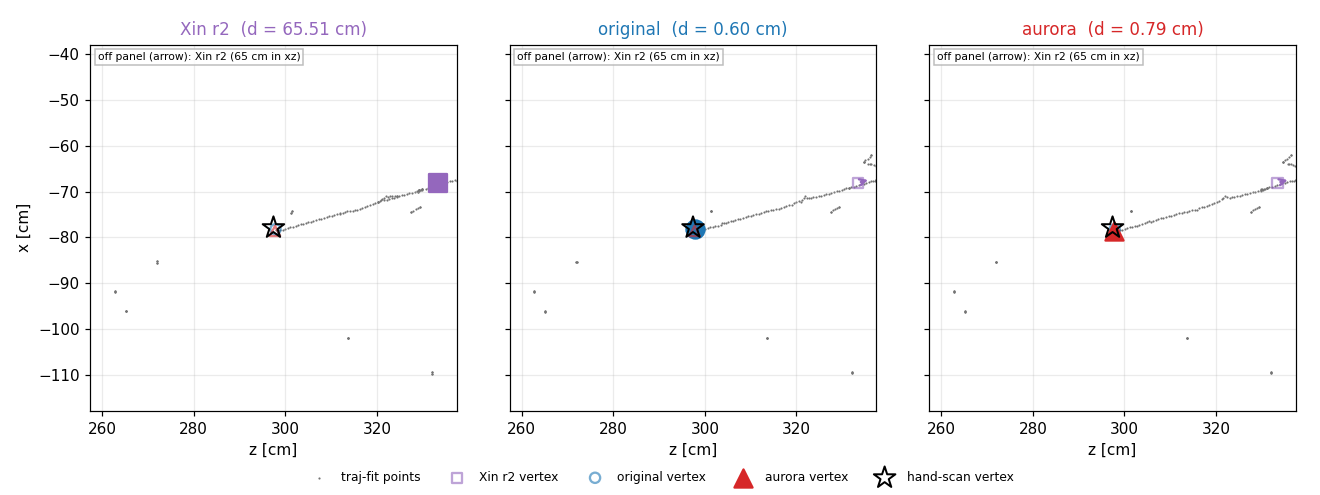
\includegraphics[width=0.92\linewidth]{figures/evt-18255-46363.png}\\[-2pt]
\scriptsize\raggedright
\textbf{Hand scan:} vertex (-77.9, 16.7, 297.4) [scanner point], Xin r2 verdict: Not OK, flavor: $\nu_e$CC\\
\textit{Scan note: close to (x, y, z) = (-77.9, 16.7, 297.4)}\\
\begin{tabular}{llcccc}
\toprule
method & & main vertex (x, y, z) cm & d to hand scan [cm] & $\nu_e$ / $\nu_\mu$ score & prediction \\
\midrule
Xin r2 & \href{https://www.phy.bnl.gov/twister/bee/set/9e2a1a1e-b637-4be5-99b7-f49bf8c04c57/event/5/}{Bee} & (-60.7, 20.4, 360.5) & 65.51 & -- & -- \\
original & \href{https://www.phy.bnl.gov/twister/bee/set/89cdea53-c227-476c-8f67-0ae765f804b4/event/33/}{Bee} & (-78.2, 16.5, 297.9) & \textbf{0.60} & 9.55 / -0.81 & $\nu_e$ \\
aurora & \href{https://www.phy.bnl.gov/twister/bee/set/431dc57f-997d-4cff-88e1-4e33fd743ab8/event/33/}{Bee} & (-78.6, 16.8, 297.8) & \textbf{0.79} & 7.89 / -0.71 & $\nu_e$ \\
\bottomrule
\end{tabular}
\end{frame}

\begin{frame}{nueCC-48: 18253/1/444187}
\vspace{-6pt}
\centering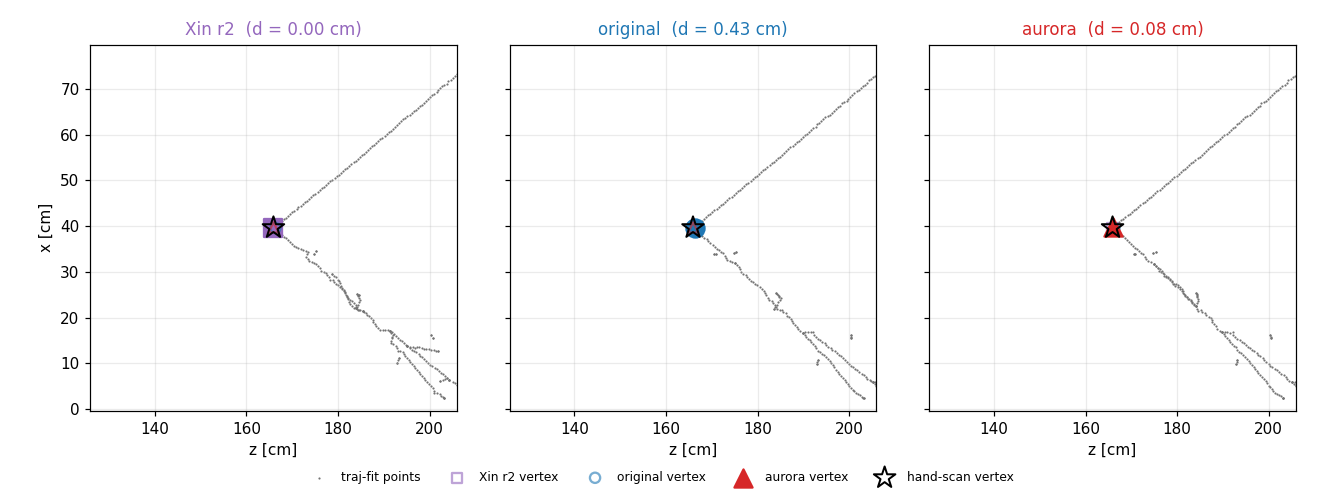
\includegraphics[width=0.92\linewidth]{figures/evt-18253-444187.png}\\[-2pt]
\scriptsize\raggedright
\textbf{Hand scan:} vertex (39.7, -12.1, 165.9) [Xin r2 vertex (scan Good/OK)], Xin r2 verdict: Good, flavor: $\nu_e$CC\\

\begin{tabular}{llcccc}
\toprule
method & & main vertex (x, y, z) cm & d to hand scan [cm] & $\nu_e$ / $\nu_\mu$ score & prediction \\
\midrule
Xin r2 & \href{https://www.phy.bnl.gov/twister/bee/set/9e2a1a1e-b637-4be5-99b7-f49bf8c04c57/event/43/}{Bee} & (39.7, -12.1, 165.9) & \textbf{0.00} & -- & -- \\
original & \href{https://www.phy.bnl.gov/twister/bee/set/89cdea53-c227-476c-8f67-0ae765f804b4/event/35/}{Bee} & (39.6, -12.2, 166.3) & \textbf{0.43} & 10.35 / 0.48 & $\nu_e$ \\
aurora & \href{https://www.phy.bnl.gov/twister/bee/set/431dc57f-997d-4cff-88e1-4e33fd743ab8/event/35/}{Bee} & (39.7, -12.2, 165.9) & \textbf{0.08} & 11.51 / 0.39 & $\nu_e$ \\
\bottomrule
\end{tabular}
\end{frame}

\begin{frame}{nueCC-48: 18255/1/138009}
\vspace{-6pt}
\centering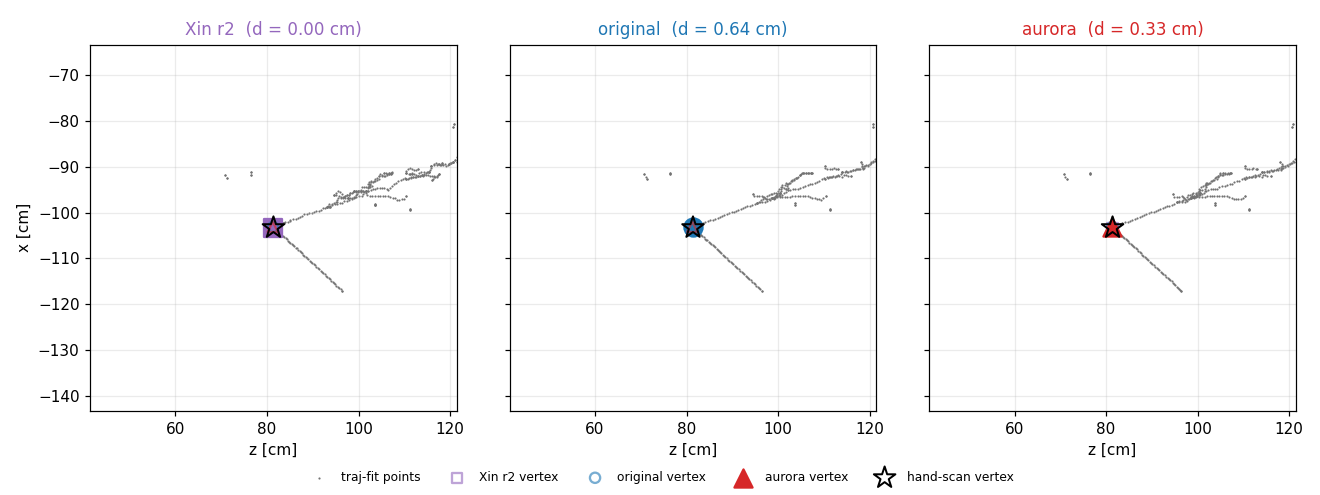
\includegraphics[width=0.92\linewidth]{figures/evt-18255-138009.png}\\[-2pt]
\scriptsize\raggedright
\textbf{Hand scan:} vertex (-103.3, 160.7, 81.4) [Xin r2 vertex (scan Good/OK)], Xin r2 verdict: Good, flavor: $\nu_e$CC\\

\begin{tabular}{llcccc}
\toprule
method & & main vertex (x, y, z) cm & d to hand scan [cm] & $\nu_e$ / $\nu_\mu$ score & prediction \\
\midrule
Xin r2 & \href{https://www.phy.bnl.gov/twister/bee/set/9e2a1a1e-b637-4be5-99b7-f49bf8c04c57/event/16/}{Bee} & (-103.3, 160.7, 81.4) & \textbf{0.00} & -- & -- \\
original & \href{https://www.phy.bnl.gov/twister/bee/set/89cdea53-c227-476c-8f67-0ae765f804b4/event/36/}{Bee} & (-103.1, 160.1, 81.3) & \textbf{0.64} & 10.03 / 0.16 & $\nu_e$ \\
aurora & \href{https://www.phy.bnl.gov/twister/bee/set/431dc57f-997d-4cff-88e1-4e33fd743ab8/event/36/}{Bee} & (-103.1, 160.5, 81.3) & \textbf{0.33} & 14.13 / -0.14 & $\nu_e$ \\
\bottomrule
\end{tabular}
\end{frame}

\begin{frame}{nueCC-48: 18255/1/423981}
\vspace{-6pt}
\centering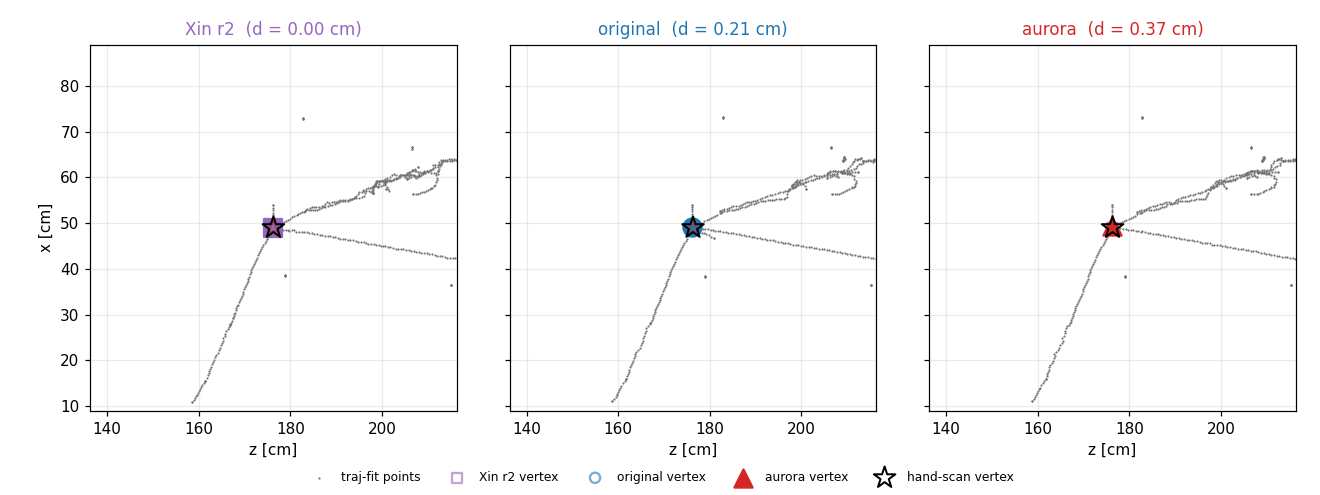
\includegraphics[width=0.92\linewidth]{figures/evt-18255-423981.png}\\[-2pt]
\scriptsize\raggedright
\textbf{Hand scan:} vertex (49.0, 141.1, 176.3) [Xin r2 vertex (scan Good/OK)], Xin r2 verdict: Good, flavor: $\nu_e$CC\\

\begin{tabular}{llcccc}
\toprule
method & & main vertex (x, y, z) cm & d to hand scan [cm] & $\nu_e$ / $\nu_\mu$ score & prediction \\
\midrule
Xin r2 & \href{https://www.phy.bnl.gov/twister/bee/set/9e2a1a1e-b637-4be5-99b7-f49bf8c04c57/event/40/}{Bee} & (49.0, 141.1, 176.3) & \textbf{0.00} & -- & -- \\
original & \href{https://www.phy.bnl.gov/twister/bee/set/89cdea53-c227-476c-8f67-0ae765f804b4/event/38/}{Bee} & (49.1, 141.2, 176.2) & \textbf{0.21} & 10.83 / 0.23 & $\nu_e$ \\
aurora & \href{https://www.phy.bnl.gov/twister/bee/set/431dc57f-997d-4cff-88e1-4e33fd743ab8/event/38/}{Bee} & (49.3, 140.9, 176.3) & \textbf{0.37} & 13.14 / 0.15 & $\nu_e$ \\
\bottomrule
\end{tabular}
\end{frame}

\begin{frame}{nueCC-48: 18255/1/433451}
\vspace{-6pt}
\centering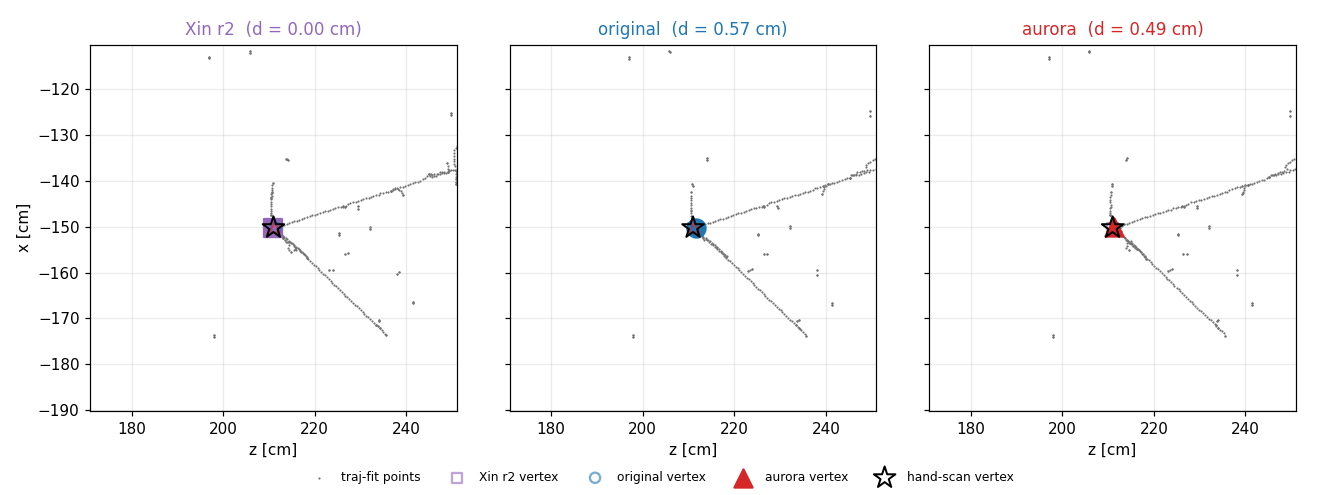
\includegraphics[width=0.92\linewidth]{figures/evt-18255-433451.png}\\[-2pt]
\scriptsize\raggedright
\textbf{Hand scan:} vertex (-150.2, 43.7, 211.0) [Xin r2 vertex (scan Good/OK)], Xin r2 verdict: Good, flavor: $\nu_e$CC\\

\begin{tabular}{llcccc}
\toprule
method & & main vertex (x, y, z) cm & d to hand scan [cm] & $\nu_e$ / $\nu_\mu$ score & prediction \\
\midrule
Xin r2 & \href{https://www.phy.bnl.gov/twister/bee/set/9e2a1a1e-b637-4be5-99b7-f49bf8c04c57/event/41/}{Bee} & (-150.2, 43.7, 211.0) & \textbf{0.00} & -- & -- \\
original & \href{https://www.phy.bnl.gov/twister/bee/set/89cdea53-c227-476c-8f67-0ae765f804b4/event/39/}{Bee} & (-150.2, 43.5, 211.5) & \textbf{0.57} & 9.19 / -0.35 & $\nu_e$ \\
aurora & \href{https://www.phy.bnl.gov/twister/bee/set/431dc57f-997d-4cff-88e1-4e33fd743ab8/event/39/}{Bee} & (-150.2, 43.3, 211.3) & \textbf{0.49} & 10.05 / -1.78 & $\nu_e$ \\
\bottomrule
\end{tabular}
\end{frame}

\begin{frame}{nueCC-48: 18259/1/54095}
\vspace{-6pt}
\centering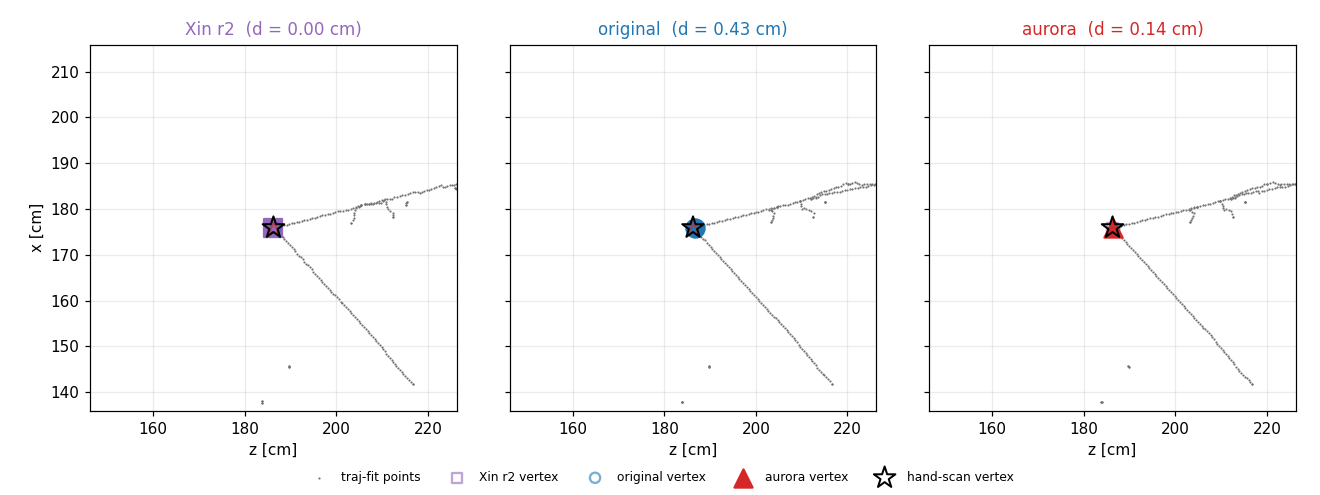
\includegraphics[width=0.92\linewidth]{figures/evt-18259-54095.png}\\[-2pt]
\scriptsize\raggedright
\textbf{Hand scan:} vertex (175.9, 27.0, 186.3) [Xin r2 vertex (scan Good/OK)], Xin r2 verdict: Good, flavor: $\nu_e$CC\\

\begin{tabular}{llcccc}
\toprule
method & & main vertex (x, y, z) cm & d to hand scan [cm] & $\nu_e$ / $\nu_\mu$ score & prediction \\
\midrule
Xin r2 & \href{https://www.phy.bnl.gov/twister/bee/set/9e2a1a1e-b637-4be5-99b7-f49bf8c04c57/event/7/}{Bee} & (175.9, 27.0, 186.3) & \textbf{0.00} & -- & -- \\
original & \href{https://www.phy.bnl.gov/twister/bee/set/89cdea53-c227-476c-8f67-0ae765f804b4/event/40/}{Bee} & (175.8, 26.9, 186.7) & \textbf{0.43} & 11.51 / -1.21 & $\nu_e$ \\
aurora & \href{https://www.phy.bnl.gov/twister/bee/set/431dc57f-997d-4cff-88e1-4e33fd743ab8/event/40/}{Bee} & (175.9, 26.9, 186.4) & \textbf{0.14} & 12.27 / -1.54 & $\nu_e$ \\
\bottomrule
\end{tabular}
\end{frame}

\begin{frame}{nueCC-48: 18355/1/400474}
\vspace{-6pt}
\centering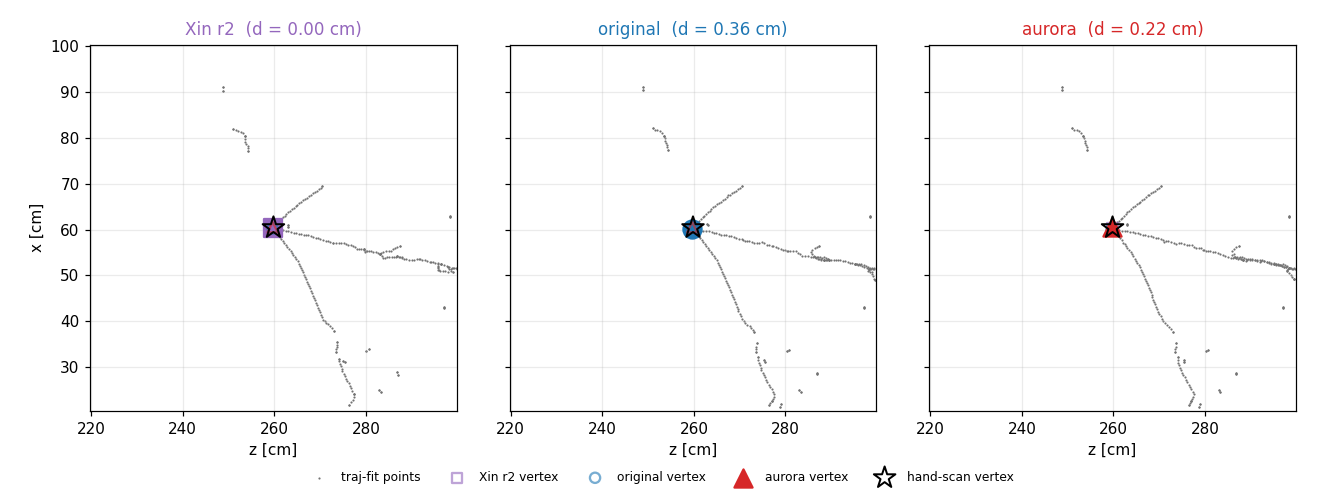
\includegraphics[width=0.92\linewidth]{figures/evt-18355-400474.png}\\[-2pt]
\scriptsize\raggedright
\textbf{Hand scan:} vertex (60.4, -117.6, 259.8) [Xin r2 vertex (scan Good/OK)], Xin r2 verdict: Good, flavor: $\nu_e$CC\\
\textit{Scan note: Shower association strange}\\
\begin{tabular}{llcccc}
\toprule
method & & main vertex (x, y, z) cm & d to hand scan [cm] & $\nu_e$ / $\nu_\mu$ score & prediction \\
\midrule
Xin r2 & \href{https://www.phy.bnl.gov/twister/bee/set/9e2a1a1e-b637-4be5-99b7-f49bf8c04c57/event/38/}{Bee} & (60.4, -117.6, 259.8) & \textbf{0.00} & -- & -- \\
original & \href{https://www.phy.bnl.gov/twister/bee/set/89cdea53-c227-476c-8f67-0ae765f804b4/event/41/}{Bee} & (60.2, -117.4, 259.6) & \textbf{0.36} & 11.79 / 0.34 & $\nu_e$ \\
aurora & \href{https://www.phy.bnl.gov/twister/bee/set/431dc57f-997d-4cff-88e1-4e33fd743ab8/event/41/}{Bee} & (60.5, -117.5, 259.6) & \textbf{0.22} & 14.02 / 0.01 & $\nu_e$ \\
\bottomrule
\end{tabular}
\end{frame}

\begin{frame}{nueCC-48: 18255/1/234638}
\vspace{-6pt}
\centering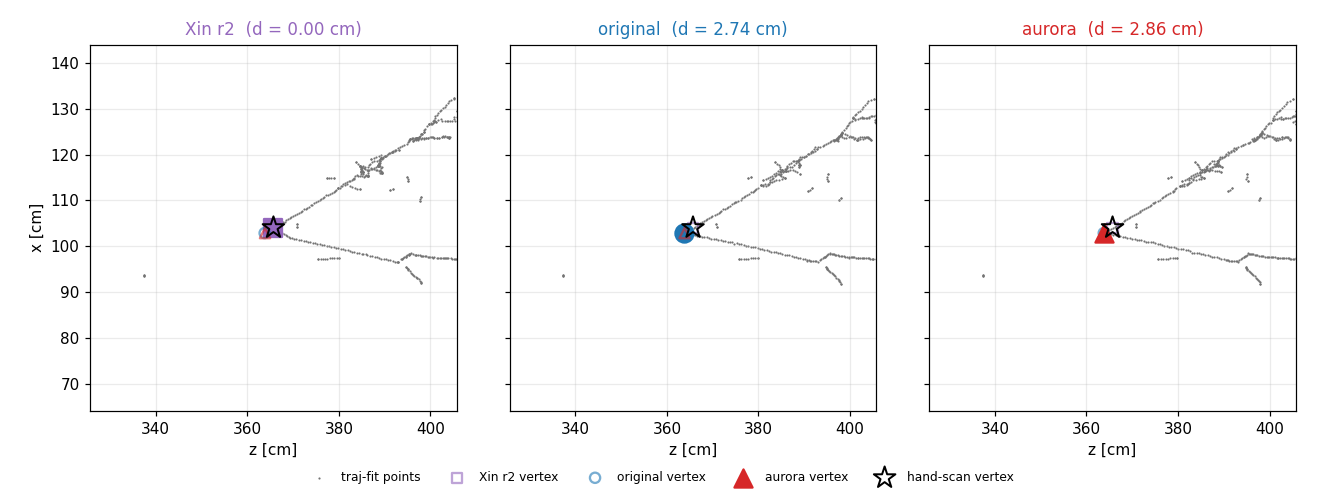
\includegraphics[width=0.92\linewidth]{figures/evt-18255-234638.png}\\[-2pt]
\scriptsize\raggedright
\textbf{Hand scan:} vertex (104.0, -4.5, 365.7) [Xin r2 vertex (scan Good/OK)], Xin r2 verdict: OK, flavor: $\nu_e$CC\\
\textit{Scan note: PR @ vertex need improvements}\\
\begin{tabular}{llcccc}
\toprule
method & & main vertex (x, y, z) cm & d to hand scan [cm] & $\nu_e$ / $\nu_\mu$ score & prediction \\
\midrule
Xin r2 & \href{https://www.phy.bnl.gov/twister/bee/set/9e2a1a1e-b637-4be5-99b7-f49bf8c04c57/event/24/}{Bee} & (104.0, -4.5, 365.7) & \textbf{0.00} & -- & -- \\
original & \href{https://www.phy.bnl.gov/twister/bee/set/89cdea53-c227-476c-8f67-0ae765f804b4/event/43/}{Bee} & (102.9, -6.0, 363.8) & 2.74 & 7.23 / 1.41 & $\nu_e$+$\nu_\mu$CC \\
aurora & \href{https://www.phy.bnl.gov/twister/bee/set/431dc57f-997d-4cff-88e1-4e33fd743ab8/event/43/}{Bee} & (102.9, -6.3, 363.9) & 2.86 & 7.45 / 1.00 & $\nu_e$+$\nu_\mu$CC \\
\bottomrule
\end{tabular}
\end{frame}

\begin{frame}{nueCC-48: 18255/1/388}
\vspace{-6pt}
\centering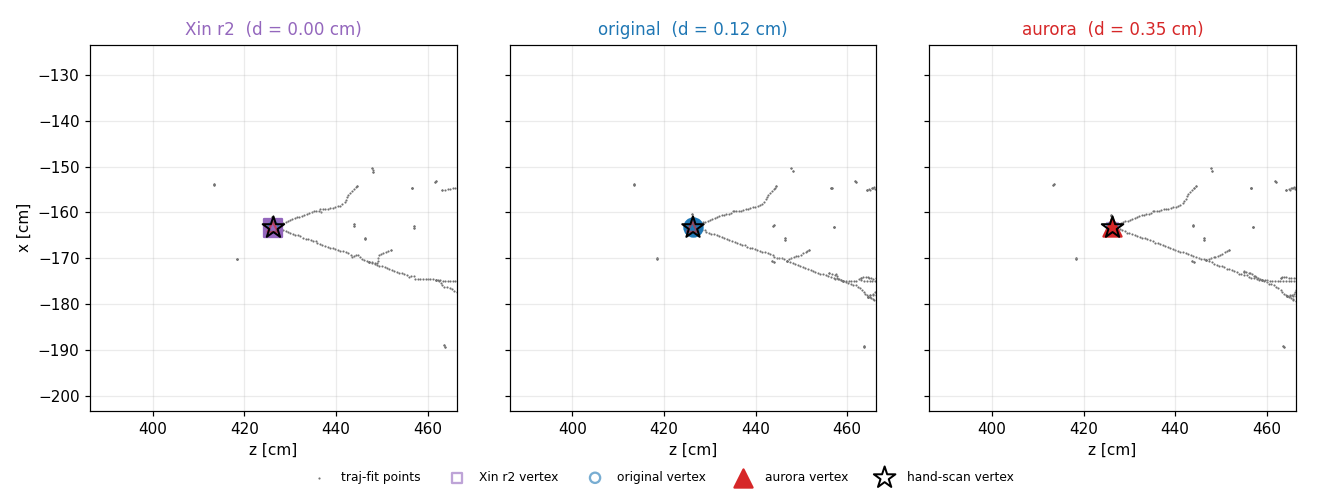
\includegraphics[width=0.92\linewidth]{figures/evt-18255-388.png}\\[-2pt]
\scriptsize\raggedright
\textbf{Hand scan:} vertex (-163.3, 31.5, 426.3) [Xin r2 vertex (scan Good/OK)], Xin r2 verdict: Good, flavor: $\nu_e$CC\\

\begin{tabular}{llcccc}
\toprule
method & & main vertex (x, y, z) cm & d to hand scan [cm] & $\nu_e$ / $\nu_\mu$ score & prediction \\
\midrule
Xin r2 & \href{https://www.phy.bnl.gov/twister/bee/set/9e2a1a1e-b637-4be5-99b7-f49bf8c04c57/event/0/}{Bee} & (-163.3, 31.5, 426.3) & \textbf{0.00} & -- & -- \\
original & \href{https://www.phy.bnl.gov/twister/bee/set/89cdea53-c227-476c-8f67-0ae765f804b4/event/44/}{Bee} & (-163.2, 31.4, 426.3) & \textbf{0.12} & 13.02 / -1.77 & $\nu_e$ \\
aurora & \href{https://www.phy.bnl.gov/twister/bee/set/431dc57f-997d-4cff-88e1-4e33fd743ab8/event/44/}{Bee} & (-163.1, 31.7, 426.2) & \textbf{0.35} & 13.95 / -1.77 & $\nu_e$ \\
\bottomrule
\end{tabular}
\end{frame}

\begin{frame}{nueCC-48: 18269/1/342199}
\vspace{-6pt}
\centering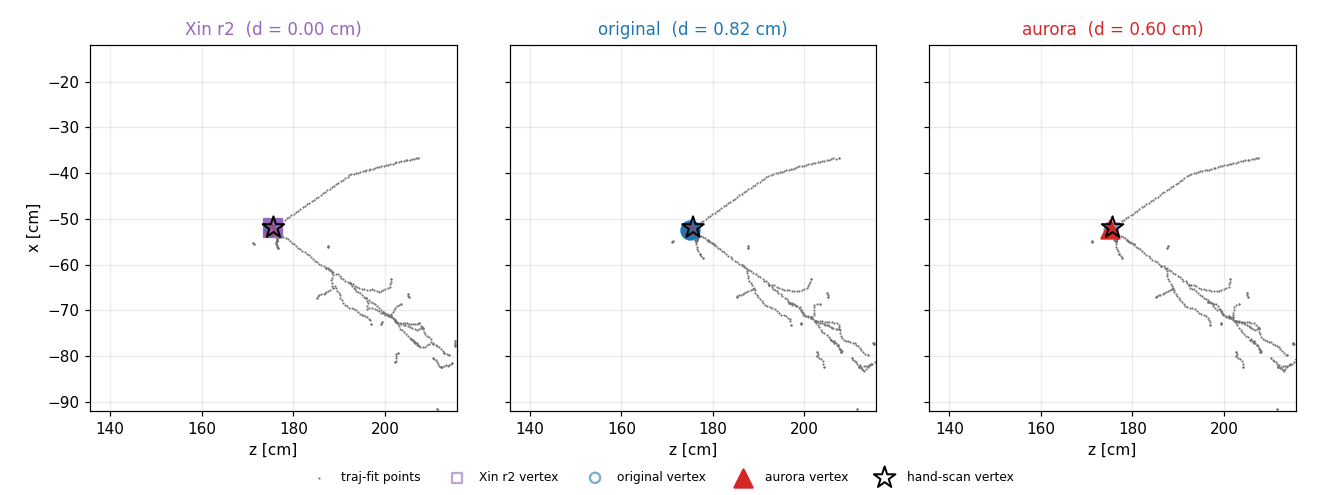
\includegraphics[width=0.92\linewidth]{figures/evt-18269-342199.png}\\[-2pt]
\scriptsize\raggedright
\textbf{Hand scan:} vertex (-51.9, 5.0, 175.7) [Xin r2 vertex (scan Good/OK)], Xin r2 verdict: OK, flavor: $\nu_e$CC\\
\textit{Scan note: PR @ vertex needs improvements OK}\\
\begin{tabular}{llcccc}
\toprule
method & & main vertex (x, y, z) cm & d to hand scan [cm] & $\nu_e$ / $\nu_\mu$ score & prediction \\
\midrule
Xin r2 & \href{https://www.phy.bnl.gov/twister/bee/set/9e2a1a1e-b637-4be5-99b7-f49bf8c04c57/event/34/}{Bee} & (-51.9, 5.0, 175.7) & \textbf{0.00} & -- & -- \\
original & \href{https://www.phy.bnl.gov/twister/bee/set/89cdea53-c227-476c-8f67-0ae765f804b4/event/46/}{Bee} & (-52.5, 5.0, 175.0) & \textbf{0.82} & 11.49 / 0.31 & $\nu_e$ \\
aurora & \href{https://www.phy.bnl.gov/twister/bee/set/431dc57f-997d-4cff-88e1-4e33fd743ab8/event/46/}{Bee} & (-52.3, 5.0, 175.2) & \textbf{0.60} & 11.30 / 0.31 & $\nu_e$ \\
\bottomrule
\end{tabular}
\end{frame}

\begin{frame}{nueCC-48: 18253/1/172230}
\vspace{-6pt}
\centering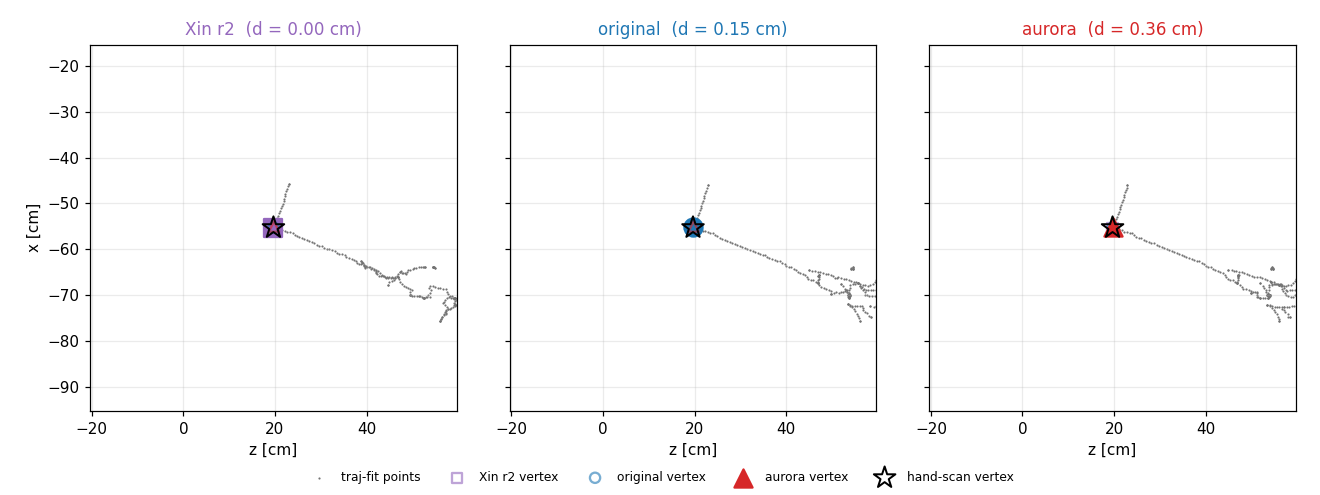
\includegraphics[width=0.92\linewidth]{figures/evt-18253-172230.png}\\[-2pt]
\scriptsize\raggedright
\textbf{Hand scan:} vertex (-55.3, -87.8, 19.7) [Xin r2 vertex (scan Good/OK)], Xin r2 verdict: Good, flavor: $\nu_e$CC\\

\begin{tabular}{llcccc}
\toprule
method & & main vertex (x, y, z) cm & d to hand scan [cm] & $\nu_e$ / $\nu_\mu$ score & prediction \\
\midrule
Xin r2 & \href{https://www.phy.bnl.gov/twister/bee/set/9e2a1a1e-b637-4be5-99b7-f49bf8c04c57/event/19/}{Bee} & (-55.3, -87.8, 19.7) & \textbf{0.00} & -- & -- \\
original & \href{https://www.phy.bnl.gov/twister/bee/set/89cdea53-c227-476c-8f67-0ae765f804b4/event/47/}{Bee} & (-55.2, -87.6, 19.7) & \textbf{0.15} & 10.62 / -1.40 & $\nu_e$ \\
aurora & \href{https://www.phy.bnl.gov/twister/bee/set/431dc57f-997d-4cff-88e1-4e33fd743ab8/event/47/}{Bee} & (-55.1, -87.5, 19.8) & \textbf{0.36} & 11.23 / -0.01 & $\nu_e$ \\
\bottomrule
\end{tabular}
\end{frame}

\begin{frame}{nueCC-48: 18259/1/74544}
\vspace{-6pt}
\centering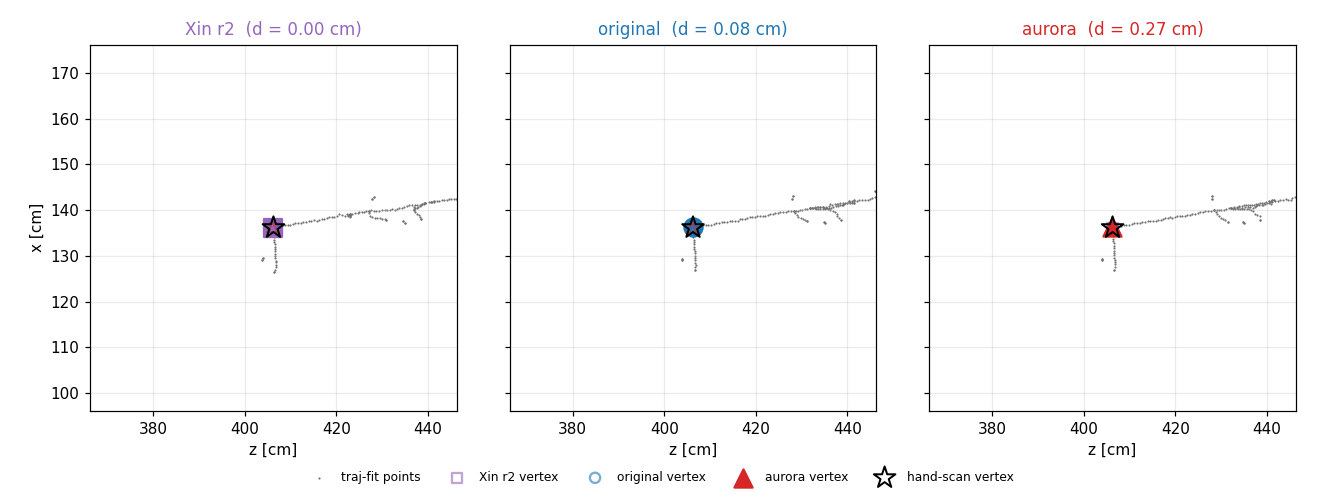
\includegraphics[width=0.92\linewidth]{figures/evt-18259-74544.png}\\[-2pt]
\scriptsize\raggedright
\textbf{Hand scan:} vertex (136.2, -170.3, 406.3) [Xin r2 vertex (scan Good/OK)], Xin r2 verdict: good, flavor: $\nu_e$CC\\

\begin{tabular}{llcccc}
\toprule
method & & main vertex (x, y, z) cm & d to hand scan [cm] & $\nu_e$ / $\nu_\mu$ score & prediction \\
\midrule
Xin r2 & \href{https://www.phy.bnl.gov/twister/bee/set/9e2a1a1e-b637-4be5-99b7-f49bf8c04c57/event/9/}{Bee} & (136.2, -170.3, 406.3) & \textbf{0.00} & -- & -- \\
original & \href{https://www.phy.bnl.gov/twister/bee/set/89cdea53-c227-476c-8f67-0ae765f804b4/event/49/}{Bee} & (136.2, -170.2, 406.2) & \textbf{0.08} & 11.06 / -0.91 & $\nu_e$ \\
aurora & \href{https://www.phy.bnl.gov/twister/bee/set/431dc57f-997d-4cff-88e1-4e33fd743ab8/event/49/}{Bee} & (136.3, -170.1, 406.1) & \textbf{0.27} & 12.53 / -0.41 & $\nu_e$ \\
\bottomrule
\end{tabular}
\end{frame}

\begin{frame}{nueCC-48: 18255/1/174637}
\vspace{-6pt}
\centering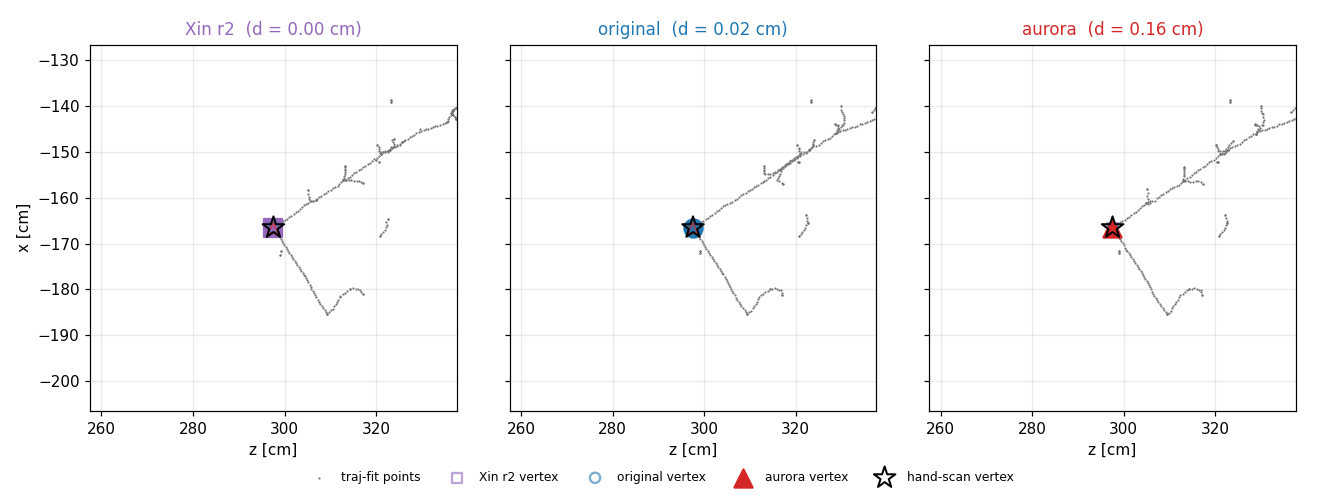
\includegraphics[width=0.92\linewidth]{figures/evt-18255-174637.png}\\[-2pt]
\scriptsize\raggedright
\textbf{Hand scan:} vertex (-166.5, -57.1, 297.6) [Xin r2 vertex (scan Good/OK)], Xin r2 verdict: Good, flavor: $\nu_e$CC\\
\textit{Scan note: Michel identified as muon. + Michel}\\
\begin{tabular}{llcccc}
\toprule
method & & main vertex (x, y, z) cm & d to hand scan [cm] & $\nu_e$ / $\nu_\mu$ score & prediction \\
\midrule
Xin r2 & \href{https://www.phy.bnl.gov/twister/bee/set/9e2a1a1e-b637-4be5-99b7-f49bf8c04c57/event/20/}{Bee} & (-166.5, -57.1, 297.6) & \textbf{0.00} & -- & -- \\
original & \href{https://www.phy.bnl.gov/twister/bee/set/89cdea53-c227-476c-8f67-0ae765f804b4/event/51/}{Bee} & (-166.5, -57.1, 297.6) & \textbf{0.02} & 10.67 / 0.81 & $\nu_e$ \\
aurora & \href{https://www.phy.bnl.gov/twister/bee/set/431dc57f-997d-4cff-88e1-4e33fd743ab8/event/51/}{Bee} & (-166.6, -57.2, 297.5) & \textbf{0.16} & 9.63 / 0.72 & $\nu_e$ \\
\bottomrule
\end{tabular}
\end{frame}

\begin{frame}{nueCC-48: 18255/1/350186}
\vspace{-6pt}
\centering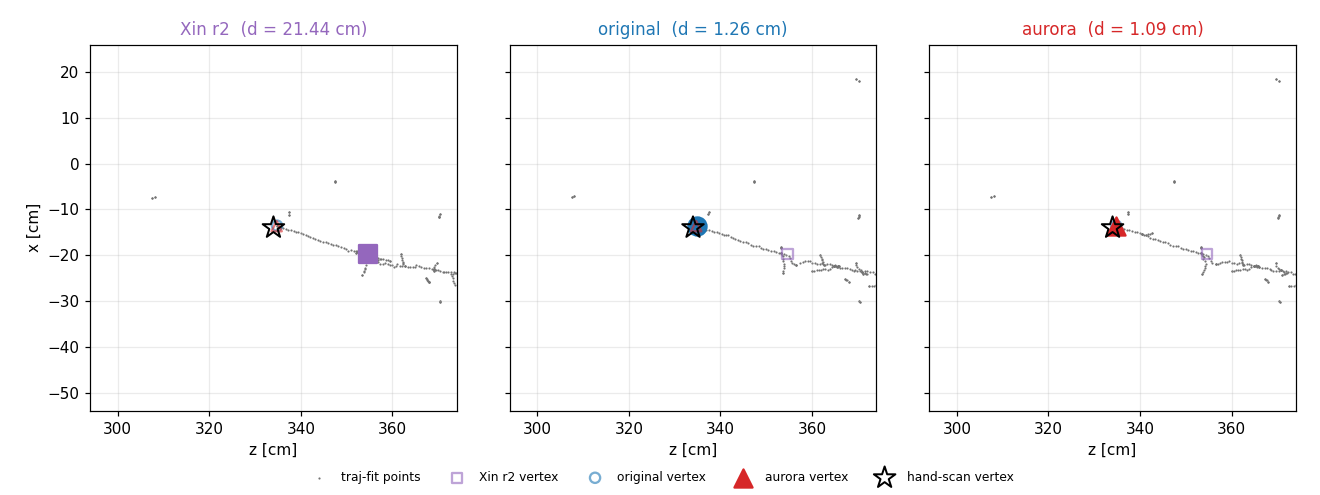
\includegraphics[width=0.92\linewidth]{figures/evt-18255-350186.png}\\[-2pt]
\scriptsize\raggedright
\textbf{Hand scan:} vertex (-14.0, 84.3, 334.0) [scanner point], Xin r2 verdict: Not good, flavor: $\nu_e$CC\\
\textit{Scan note: close to (x, y, z) = (-14.0, 84.3, 334.0)}\\
\begin{tabular}{llcccc}
\toprule
method & & main vertex (x, y, z) cm & d to hand scan [cm] & $\nu_e$ / $\nu_\mu$ score & prediction \\
\midrule
Xin r2 & \href{https://www.phy.bnl.gov/twister/bee/set/9e2a1a1e-b637-4be5-99b7-f49bf8c04c57/event/35/}{Bee} & (-19.8, 83.1, 354.6) & 21.44 & -- & -- \\
original & \href{https://www.phy.bnl.gov/twister/bee/set/89cdea53-c227-476c-8f67-0ae765f804b4/event/52/}{Bee} & (-13.6, 83.4, 334.8) & 1.26 & 9.51 / -1.52 & $\nu_e$ \\
aurora & \href{https://www.phy.bnl.gov/twister/bee/set/431dc57f-997d-4cff-88e1-4e33fd743ab8/event/52/}{Bee} & (-13.7, 83.5, 334.7) & 1.09 & 12.30 / -1.59 & $\nu_e$ \\
\bottomrule
\end{tabular}
\end{frame}

\begin{frame}{nueCC-48: 18255/1/422851}
\vspace{-6pt}
\centering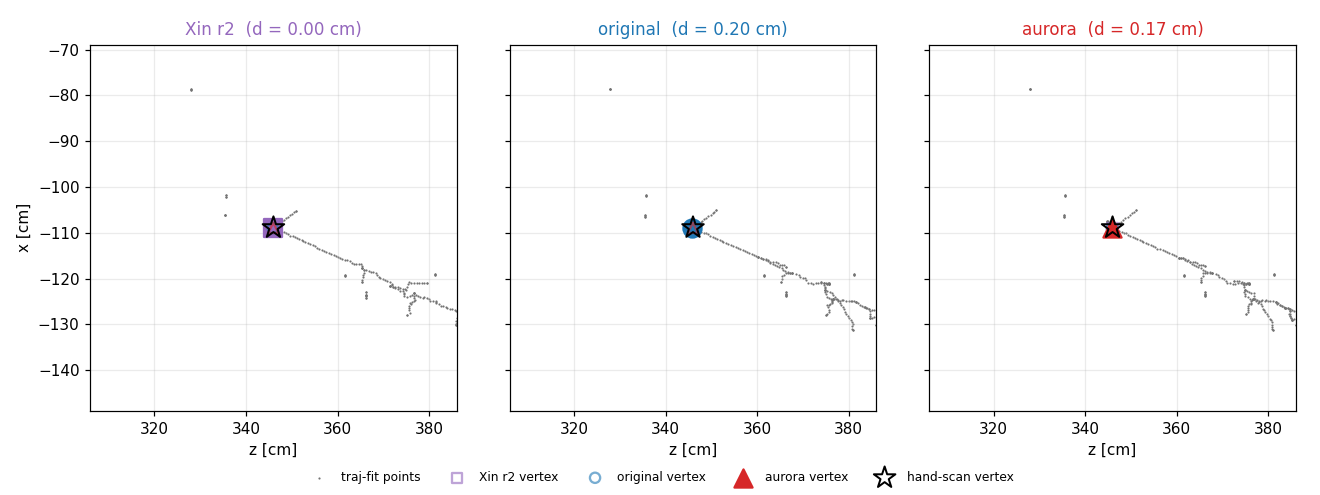
\includegraphics[width=0.92\linewidth]{figures/evt-18255-422851.png}\\[-2pt]
\scriptsize\raggedright
\textbf{Hand scan:} vertex (-108.9, -59.4, 346.0) [Xin r2 vertex (scan Good/OK)], Xin r2 verdict: Good, flavor: $\nu_e$CC\\

\begin{tabular}{llcccc}
\toprule
method & & main vertex (x, y, z) cm & d to hand scan [cm] & $\nu_e$ / $\nu_\mu$ score & prediction \\
\midrule
Xin r2 & \href{https://www.phy.bnl.gov/twister/bee/set/9e2a1a1e-b637-4be5-99b7-f49bf8c04c57/event/39/}{Bee} & (-108.9, -59.4, 346.0) & \textbf{0.00} & -- & -- \\
original & \href{https://www.phy.bnl.gov/twister/bee/set/89cdea53-c227-476c-8f67-0ae765f804b4/event/53/}{Bee} & (-109.0, -59.4, 345.8) & \textbf{0.20} & 13.06 / -1.08 & $\nu_e$ \\
aurora & \href{https://www.phy.bnl.gov/twister/bee/set/431dc57f-997d-4cff-88e1-4e33fd743ab8/event/53/}{Bee} & (-108.9, -59.5, 346.0) & \textbf{0.17} & 14.38 / -1.27 & $\nu_e$ \\
\bottomrule
\end{tabular}
\end{frame}

\begin{frame}{nueCC-48: 18255/1/389538}
\vspace{-6pt}
\centering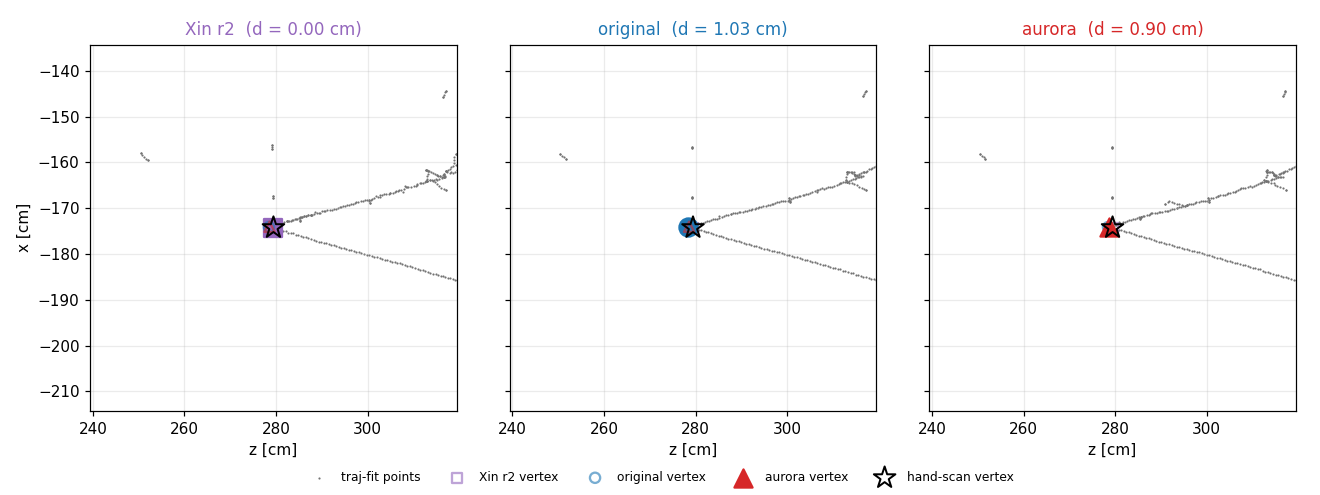
\includegraphics[width=0.92\linewidth]{figures/evt-18255-389538.png}\\[-2pt]
\scriptsize\raggedright
\textbf{Hand scan:} vertex (-174.3, 2.8, 279.4) [Xin r2 vertex (scan Good/OK)], Xin r2 verdict: Good, flavor: $\nu_e$CC\\
\textit{Scan note: second neutrino ided as gamma}\\
\begin{tabular}{llcccc}
\toprule
method & & main vertex (x, y, z) cm & d to hand scan [cm] & $\nu_e$ / $\nu_\mu$ score & prediction \\
\midrule
Xin r2 & \href{https://www.phy.bnl.gov/twister/bee/set/9e2a1a1e-b637-4be5-99b7-f49bf8c04c57/event/37/}{Bee} & (-174.3, 2.8, 279.4) & \textbf{0.00} & -- & -- \\
original & \href{https://www.phy.bnl.gov/twister/bee/set/89cdea53-c227-476c-8f67-0ae765f804b4/event/54/}{Bee} & (-174.1, 2.5, 278.4) & 1.03 & 10.91 / 0.49 & $\nu_e$ \\
aurora & \href{https://www.phy.bnl.gov/twister/bee/set/431dc57f-997d-4cff-88e1-4e33fd743ab8/event/54/}{Bee} & (-174.1, 2.5, 278.6) & \textbf{0.90} & 15.05 / -0.16 & $\nu_e$ \\
\bottomrule
\end{tabular}
\end{frame}

\begin{frame}{nueCC-48: 18255/1/447477}
\vspace{-6pt}
\centering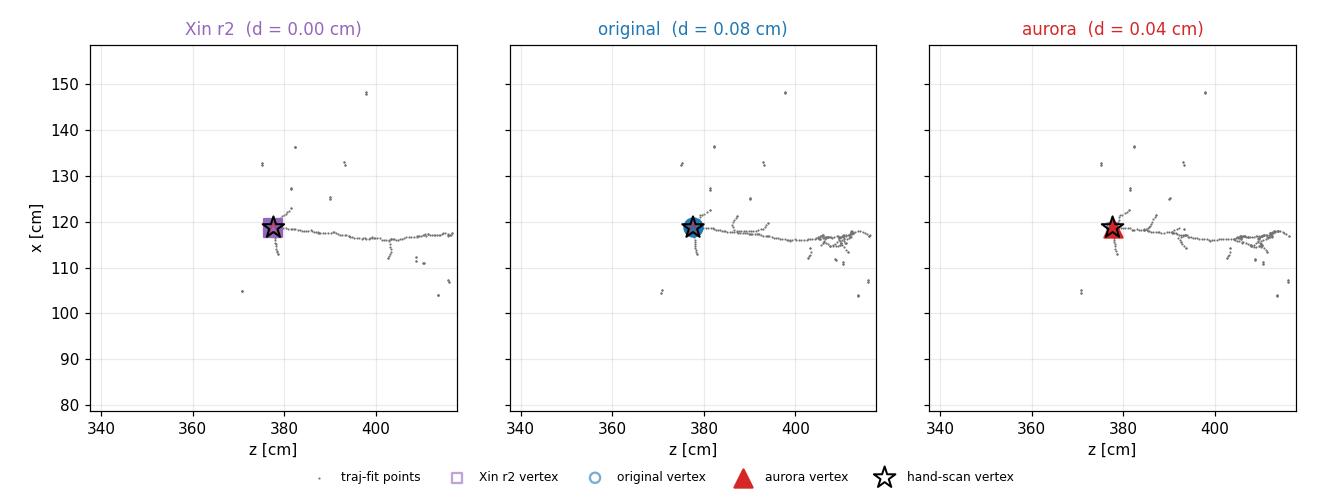
\includegraphics[width=0.92\linewidth]{figures/evt-18255-447477.png}\\[-2pt]
\scriptsize\raggedright
\textbf{Hand scan:} vertex (118.7, -29.7, 377.6) [Xin r2 vertex (scan Good/OK)], Xin r2 verdict: Good, flavor: $\nu_e$CC\\
\textit{Scan note: electron ided as proton trunk ...}\\
\begin{tabular}{llcccc}
\toprule
method & & main vertex (x, y, z) cm & d to hand scan [cm] & $\nu_e$ / $\nu_\mu$ score & prediction \\
\midrule
Xin r2 & \href{https://www.phy.bnl.gov/twister/bee/set/9e2a1a1e-b637-4be5-99b7-f49bf8c04c57/event/44/}{Bee} & (118.7, -29.7, 377.6) & \textbf{0.00} & -- & -- \\
original & \href{https://www.phy.bnl.gov/twister/bee/set/89cdea53-c227-476c-8f67-0ae765f804b4/event/56/}{Bee} & (118.8, -29.6, 377.6) & \textbf{0.08} & 10.90 / 0.00 & $\nu_e$ \\
aurora & \href{https://www.phy.bnl.gov/twister/bee/set/431dc57f-997d-4cff-88e1-4e33fd743ab8/event/56/}{Bee} & (118.7, -29.7, 377.6) & \textbf{0.04} & 11.67 / -0.16 & $\nu_e$ \\
\bottomrule
\end{tabular}
\end{frame}

\begin{frame}{nueCC-48: 18255/1/239794}
\vspace{-6pt}
\centering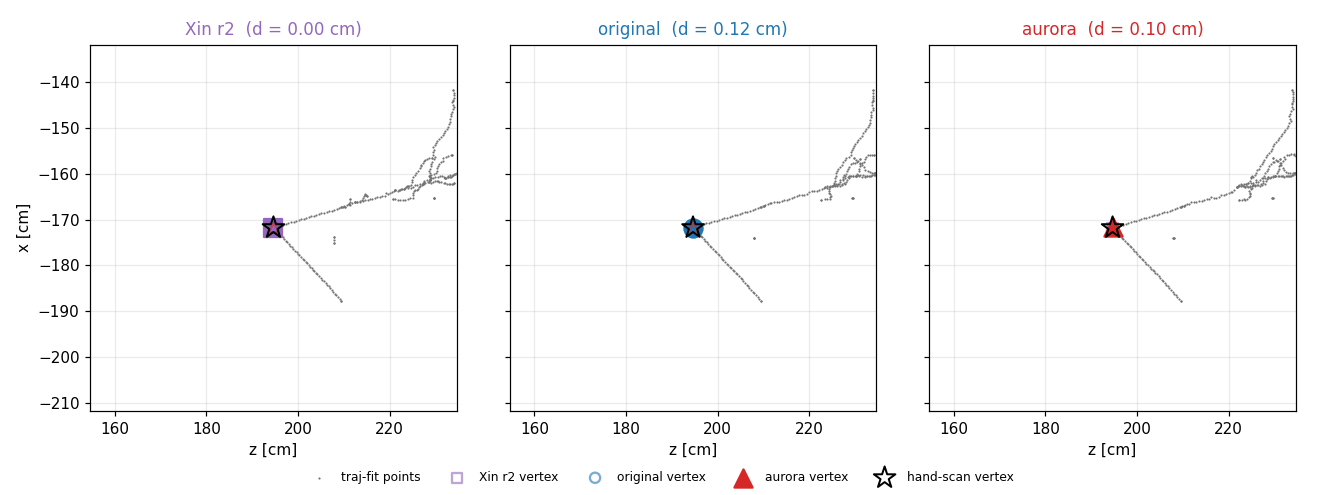
\includegraphics[width=0.92\linewidth]{figures/evt-18255-239794.png}\\[-2pt]
\scriptsize\raggedright
\textbf{Hand scan:} vertex (-171.8, -26.5, 194.6) [Xin r2 vertex (scan Good/OK)], Xin r2 verdict: Good, flavor: $\nu_e$CC\\

\begin{tabular}{llcccc}
\toprule
method & & main vertex (x, y, z) cm & d to hand scan [cm] & $\nu_e$ / $\nu_\mu$ score & prediction \\
\midrule
Xin r2 & \href{https://www.phy.bnl.gov/twister/bee/set/9e2a1a1e-b637-4be5-99b7-f49bf8c04c57/event/26/}{Bee} & (-171.8, -26.5, 194.6) & \textbf{0.00} & -- & -- \\
original & \href{https://www.phy.bnl.gov/twister/bee/set/89cdea53-c227-476c-8f67-0ae765f804b4/event/57/}{Bee} & (-171.7, -26.6, 194.7) & \textbf{0.12} & 13.05 / -0.59 & $\nu_e$ \\
aurora & \href{https://www.phy.bnl.gov/twister/bee/set/431dc57f-997d-4cff-88e1-4e33fd743ab8/event/57/}{Bee} & (-171.7, -26.4, 194.7) & \textbf{0.10} & 12.89 / -0.75 & $\nu_e$ \\
\bottomrule
\end{tabular}
\end{frame}

\begin{frame}{nueCC-48: 18313/1/81597}
\vspace{-6pt}
\centering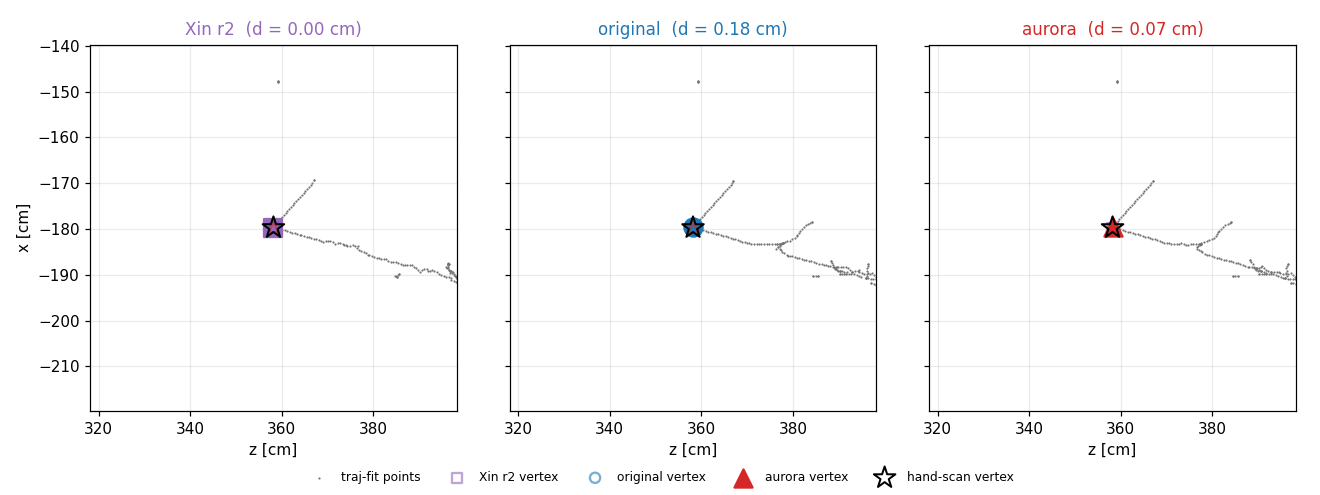
\includegraphics[width=0.92\linewidth]{figures/evt-18313-81597.png}\\[-2pt]
\scriptsize\raggedright
\textbf{Hand scan:} vertex (-179.7, 39.9, 358.2) [Xin r2 vertex (scan Good/OK)], Xin r2 verdict: Good, flavor: $\nu_e$CC\\

\begin{tabular}{llcccc}
\toprule
method & & main vertex (x, y, z) cm & d to hand scan [cm] & $\nu_e$ / $\nu_\mu$ score & prediction \\
\midrule
Xin r2 & \href{https://www.phy.bnl.gov/twister/bee/set/9e2a1a1e-b637-4be5-99b7-f49bf8c04c57/event/10/}{Bee} & (-179.7, 39.9, 358.2) & \textbf{0.00} & -- & -- \\
original & \href{https://www.phy.bnl.gov/twister/bee/set/89cdea53-c227-476c-8f67-0ae765f804b4/event/58/}{Bee} & (-179.6, 40.0, 358.3) & \textbf{0.18} & 14.40 / 0.36 & $\nu_e$ \\
aurora & \href{https://www.phy.bnl.gov/twister/bee/set/431dc57f-997d-4cff-88e1-4e33fd743ab8/event/58/}{Bee} & (-179.7, 40.0, 358.2) & \textbf{0.07} & 12.25 / 0.25 & $\nu_e$ \\
\bottomrule
\end{tabular}
\end{frame}

\begin{frame}{nueCC-48: 18306/1/256587}
\vspace{-6pt}
\centering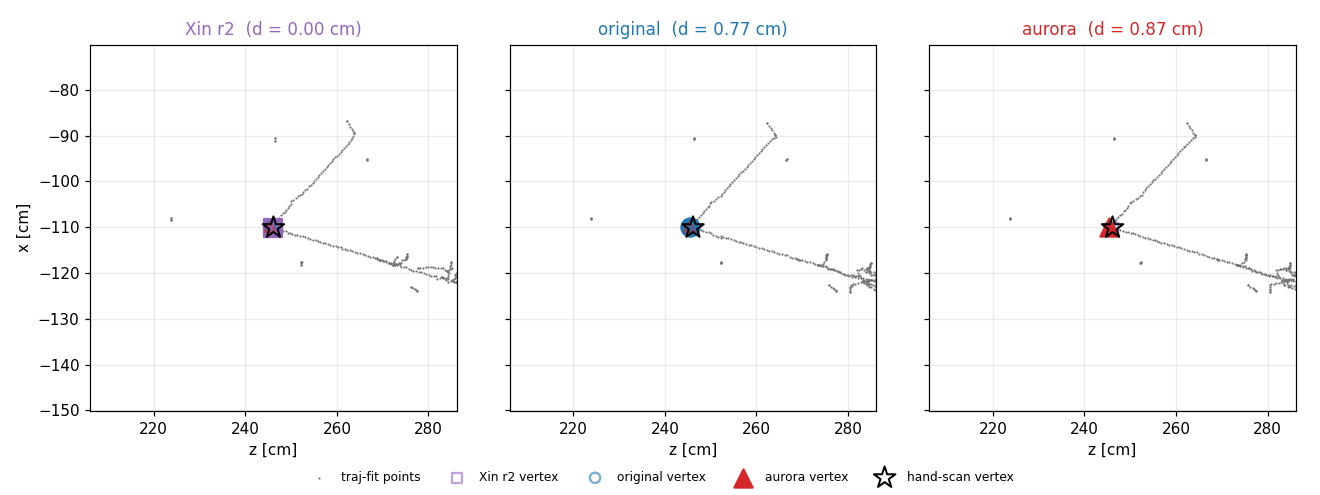
\includegraphics[width=0.92\linewidth]{figures/evt-18306-256587.png}\\[-2pt]
\scriptsize\raggedright
\textbf{Hand scan:} vertex (-110.1, -25.5, 246.1) [Xin r2 vertex (scan Good/OK)], Xin r2 verdict: Good, flavor: $\nu_e$CC\\
\textit{Scan note: track identified as electron}\\
\begin{tabular}{llcccc}
\toprule
method & & main vertex (x, y, z) cm & d to hand scan [cm] & $\nu_e$ / $\nu_\mu$ score & prediction \\
\midrule
Xin r2 & \href{https://www.phy.bnl.gov/twister/bee/set/9e2a1a1e-b637-4be5-99b7-f49bf8c04c57/event/28/}{Bee} & (-110.1, -25.5, 246.1) & \textbf{0.00} & -- & -- \\
original & \href{https://www.phy.bnl.gov/twister/bee/set/89cdea53-c227-476c-8f67-0ae765f804b4/event/59/}{Bee} & (-109.9, -25.1, 245.5) & \textbf{0.77} & 10.34 / -1.09 & $\nu_e$ \\
aurora & \href{https://www.phy.bnl.gov/twister/bee/set/431dc57f-997d-4cff-88e1-4e33fd743ab8/event/59/}{Bee} & (-109.9, -25.1, 245.4) & \textbf{0.87} & 10.93 / -1.06 & $\nu_e$ \\
\bottomrule
\end{tabular}
\end{frame}

\begin{frame}{nueCC-48: 18255/1/489330}
\vspace{-6pt}
\centering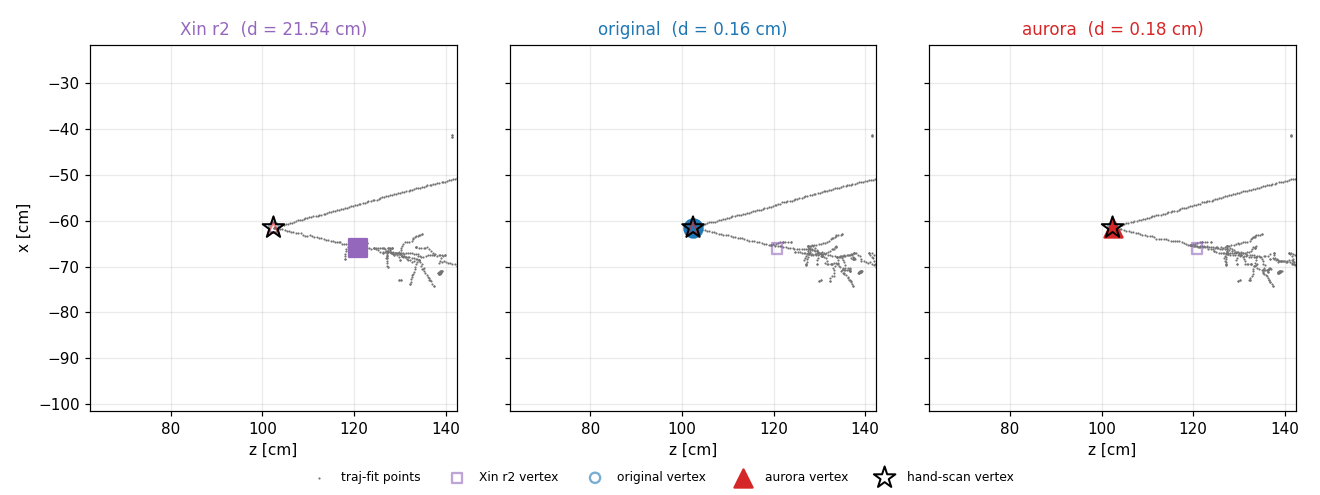
\includegraphics[width=0.92\linewidth]{figures/evt-18255-489330.png}\\[-2pt]
\scriptsize\raggedright
\textbf{Hand scan:} vertex (-61.5, -159.1, 102.4) [scanner point], Xin r2 verdict: Not good, flavor: $\nu_e$CC\\
\textit{Scan note: close to (x, y, z) = (-61.5, -159.1, 102.4)}\\
\begin{tabular}{llcccc}
\toprule
method & & main vertex (x, y, z) cm & d to hand scan [cm] & $\nu_e$ / $\nu_\mu$ score & prediction \\
\midrule
Xin r2 & \href{https://www.phy.bnl.gov/twister/bee/set/9e2a1a1e-b637-4be5-99b7-f49bf8c04c57/event/46/}{Bee} & (-66.0, -169.3, 120.8) & 21.54 & -- & -- \\
original & \href{https://www.phy.bnl.gov/twister/bee/set/89cdea53-c227-476c-8f67-0ae765f804b4/event/60/}{Bee} & (-61.5, -159.0, 102.5) & \textbf{0.16} & 12.94 / 0.06 & $\nu_e$ \\
aurora & \href{https://www.phy.bnl.gov/twister/bee/set/431dc57f-997d-4cff-88e1-4e33fd743ab8/event/60/}{Bee} & (-61.5, -158.9, 102.4) & \textbf{0.18} & 13.87 / -1.36 & $\nu_e$ \\
\bottomrule
\end{tabular}
\end{frame}

\begin{frame}{nueCC-48: 18255/1/246579}
\vspace{-6pt}
\centering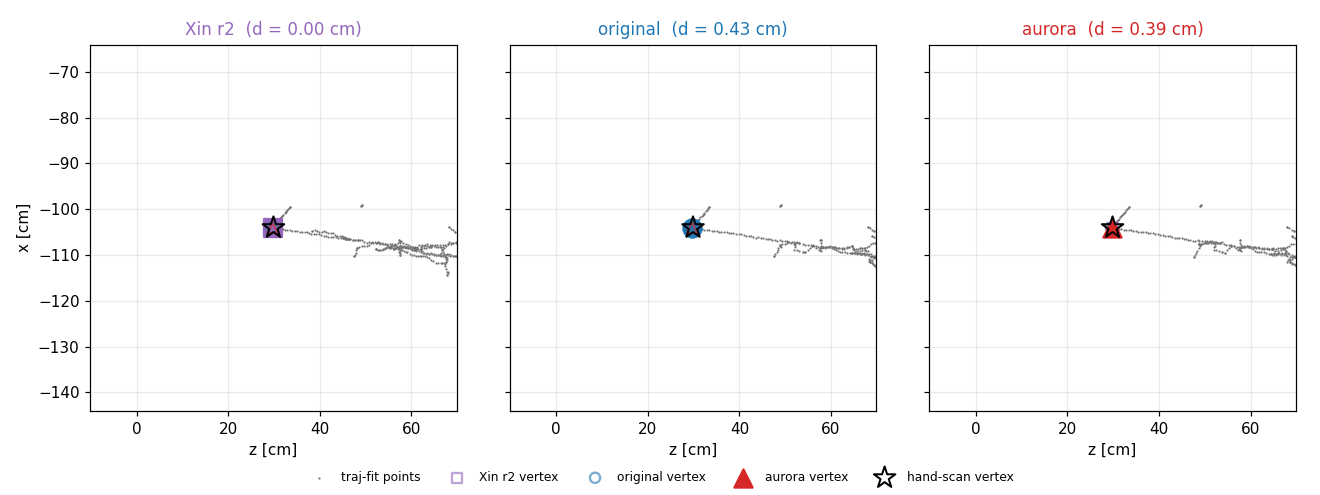
\includegraphics[width=0.92\linewidth]{figures/evt-18255-246579.png}\\[-2pt]
\scriptsize\raggedright
\textbf{Hand scan:} vertex (-104.0, -59.0, 29.9) [Xin r2 vertex (scan Good/OK)], Xin r2 verdict: Good, flavor: $\nu_e$CC\\

\begin{tabular}{llcccc}
\toprule
method & & main vertex (x, y, z) cm & d to hand scan [cm] & $\nu_e$ / $\nu_\mu$ score & prediction \\
\midrule
Xin r2 & \href{https://www.phy.bnl.gov/twister/bee/set/9e2a1a1e-b637-4be5-99b7-f49bf8c04c57/event/27/}{Bee} & (-104.0, -59.0, 29.9) & \textbf{0.00} & -- & -- \\
original & \href{https://www.phy.bnl.gov/twister/bee/set/89cdea53-c227-476c-8f67-0ae765f804b4/event/61/}{Bee} & (-104.1, -58.7, 29.6) & \textbf{0.43} & 11.45 / -0.46 & $\nu_e$ \\
aurora & \href{https://www.phy.bnl.gov/twister/bee/set/431dc57f-997d-4cff-88e1-4e33fd743ab8/event/61/}{Bee} & (-104.0, -58.7, 29.7) & \textbf{0.39} & 13.57 / -0.49 & $\nu_e$ \\
\bottomrule
\end{tabular}
\end{frame}

\begin{frame}{nueCC-48: 18259/1/131357}
\vspace{-6pt}
\centering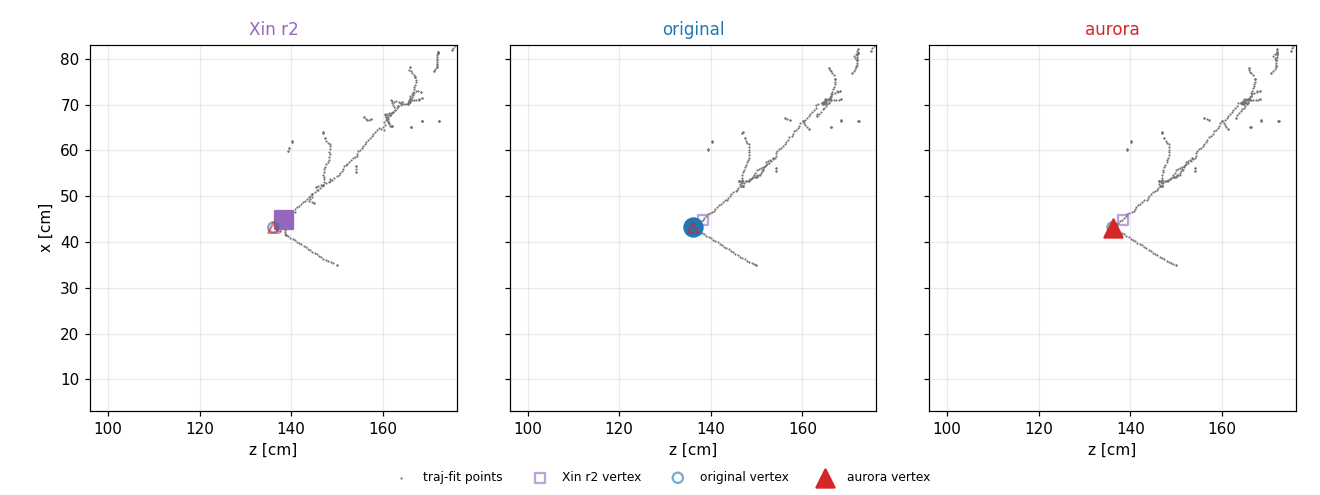
\includegraphics[width=0.92\linewidth]{figures/evt-18259-131357.png}\\[-2pt]
\scriptsize\raggedright
\textbf{Hand scan:} vertex -- [none], Xin r2 verdict: Not good, flavor: $\nu_e$CC\\
\textit{Scan note: PR @ vertex need improvements}\\
\begin{tabular}{llcccc}
\toprule
method & & main vertex (x, y, z) cm & d to hand scan [cm] & $\nu_e$ / $\nu_\mu$ score & prediction \\
\midrule
Xin r2 & \href{https://www.phy.bnl.gov/twister/bee/set/9e2a1a1e-b637-4be5-99b7-f49bf8c04c57/event/14/}{Bee} & (44.9, 176.3, 138.3) & -- & -- & -- \\
original & \href{https://www.phy.bnl.gov/twister/bee/set/89cdea53-c227-476c-8f67-0ae765f804b4/event/62/}{Bee} & (43.2, 177.6, 136.1) & -- & 11.61 / -0.69 & $\nu_e$ \\
aurora & \href{https://www.phy.bnl.gov/twister/bee/set/431dc57f-997d-4cff-88e1-4e33fd743ab8/event/62/}{Bee} & (43.1, 177.6, 136.1) & -- & 11.57 / -0.71 & $\nu_e$ \\
\bottomrule
\end{tabular}
\end{frame}

\begin{frame}{nueCC-48: 18409/1/214469}
\vspace{-6pt}
\centering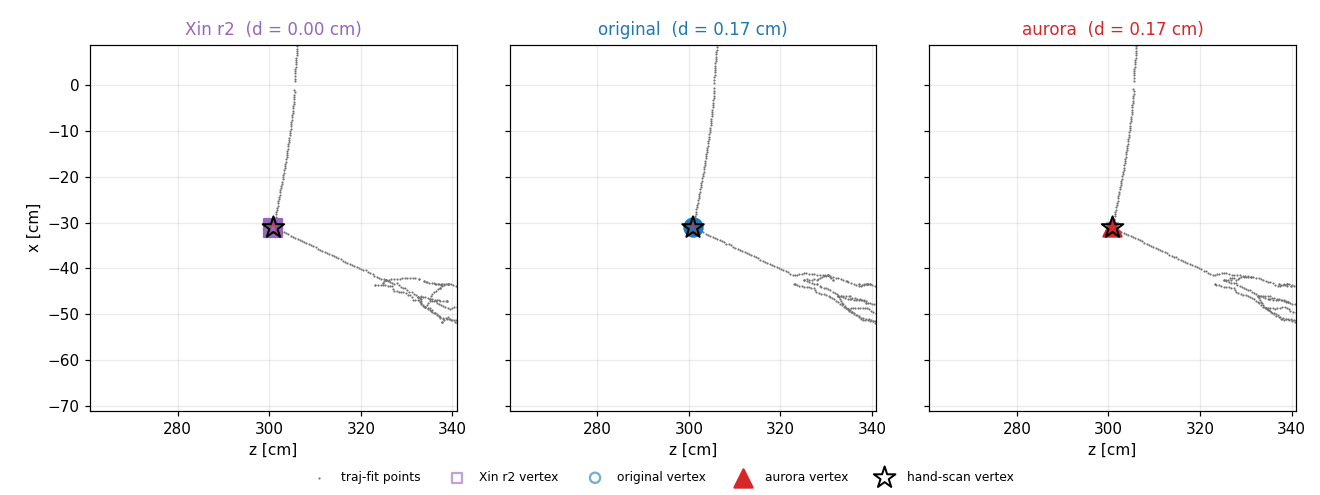
\includegraphics[width=0.92\linewidth]{figures/evt-18409-214469.png}\\[-2pt]
\scriptsize\raggedright
\textbf{Hand scan:} vertex (-31.1, 2.8, 300.9) [Xin r2 vertex (scan Good/OK)], Xin r2 verdict: Good, flavor: $\nu_e$CC\\
\textit{Scan note: electron identified as pi0?}\\
\begin{tabular}{llcccc}
\toprule
method & & main vertex (x, y, z) cm & d to hand scan [cm] & $\nu_e$ / $\nu_\mu$ score & prediction \\
\midrule
Xin r2 & \href{https://www.phy.bnl.gov/twister/bee/set/9e2a1a1e-b637-4be5-99b7-f49bf8c04c57/event/22/}{Bee} & (-31.1, 2.8, 300.9) & \textbf{0.00} & -- & -- \\
original & \href{https://www.phy.bnl.gov/twister/bee/set/89cdea53-c227-476c-8f67-0ae765f804b4/event/63/}{Bee} & (-31.0, 2.6, 300.9) & \textbf{0.17} & 11.65 / -1.31 & $\nu_e$ \\
aurora & \href{https://www.phy.bnl.gov/twister/bee/set/431dc57f-997d-4cff-88e1-4e33fd743ab8/event/63/}{Bee} & (-31.0, 2.6, 300.9) & \textbf{0.17} & 10.96 / -1.45 & $\nu_e$ \\
\bottomrule
\end{tabular}
\end{frame}

\begin{frame}{nueCC-48: 18255/1/219295}
\vspace{-6pt}
\centering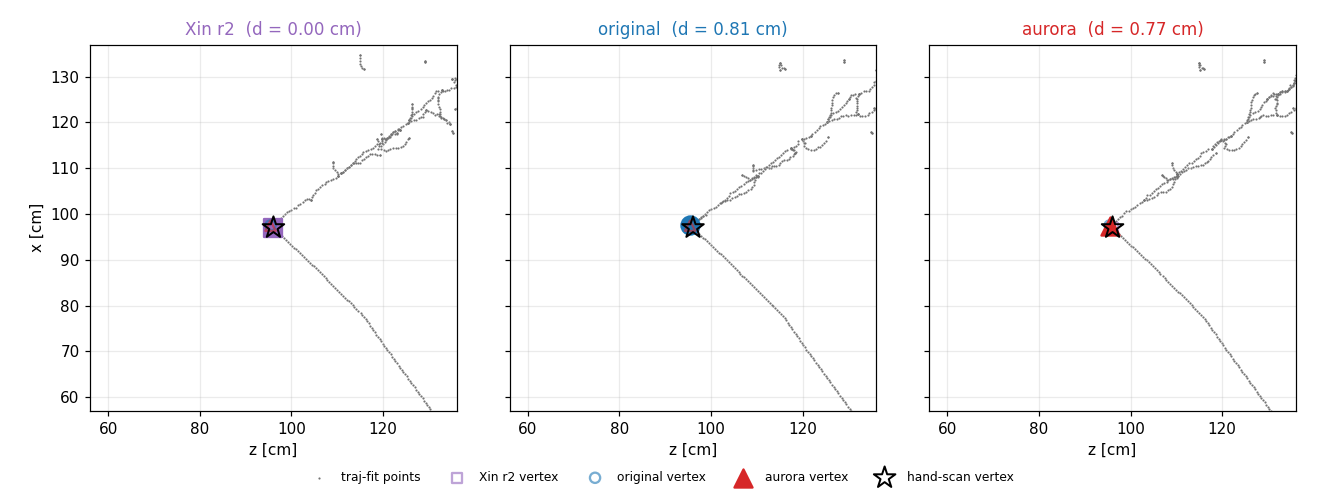
\includegraphics[width=0.92\linewidth]{figures/evt-18255-219295.png}\\[-2pt]
\scriptsize\raggedright
\textbf{Hand scan:} vertex (97.0, 52.4, 96.1) [Xin r2 vertex (scan Good/OK)], Xin r2 verdict: Good, flavor: $\nu_e$CC\\

\begin{tabular}{llcccc}
\toprule
method & & main vertex (x, y, z) cm & d to hand scan [cm] & $\nu_e$ / $\nu_\mu$ score & prediction \\
\midrule
Xin r2 & \href{https://www.phy.bnl.gov/twister/bee/set/9e2a1a1e-b637-4be5-99b7-f49bf8c04c57/event/23/}{Bee} & (97.0, 52.4, 96.1) & \textbf{0.00} & -- & -- \\
original & \href{https://www.phy.bnl.gov/twister/bee/set/89cdea53-c227-476c-8f67-0ae765f804b4/event/64/}{Bee} & (97.5, 52.4, 95.4) & \textbf{0.81} & 9.84 / -1.08 & $\nu_e$ \\
aurora & \href{https://www.phy.bnl.gov/twister/bee/set/431dc57f-997d-4cff-88e1-4e33fd743ab8/event/64/}{Bee} & (97.4, 52.4, 95.4) & \textbf{0.77} & 8.84 / -1.33 & $\nu_e$ \\
\bottomrule
\end{tabular}
\end{frame}

\begin{frame}{nueCC-48: 18255/1/10550}
\vspace{-6pt}
\centering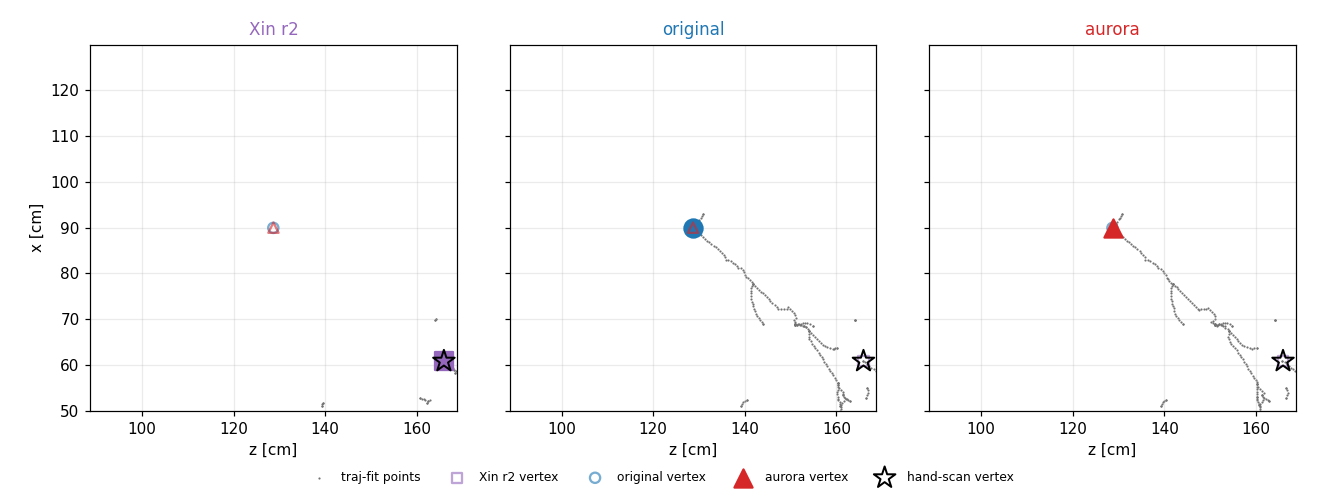
\includegraphics[width=0.92\linewidth]{figures/evt-18255-10550.png}\\[-2pt]
\scriptsize\raggedright
\textbf{Hand scan:} vertex (60.8, 55.0, 165.9) [Xin r2 vertex (scan Good/OK)], Xin r2 verdict: OK, flavor: $\nu_e$CC; \textcolor{orange!80!black}{our candidate $\ne$ scanned interaction}\\
\textit{Scan note: main event missing ... separated, but mergd again???}\\
\begin{tabular}{llcccc}
\toprule
method & & main vertex (x, y, z) cm & d to hand scan [cm] & $\nu_e$ / $\nu_\mu$ score & prediction \\
\midrule
Xin r2 & \href{https://www.phy.bnl.gov/twister/bee/set/9e2a1a1e-b637-4be5-99b7-f49bf8c04c57/event/1/}{Bee} & (60.8, 55.0, 165.9) & -- & -- & -- \\
original & \href{https://www.phy.bnl.gov/twister/bee/set/89cdea53-c227-476c-8f67-0ae765f804b4/event/65/}{Bee} & (89.9, 55.0, 128.7) & -- & 13.23 / -0.38 & $\nu_e$ \\
aurora & \href{https://www.phy.bnl.gov/twister/bee/set/431dc57f-997d-4cff-88e1-4e33fd743ab8/event/65/}{Bee} & (90.0, 55.0, 128.7) & -- & 12.65 / -0.39 & $\nu_e$ \\
\bottomrule
\end{tabular}
\end{frame}

\begin{frame}{nueCC-48: 18279/1/267597}
\vspace{-6pt}
\centering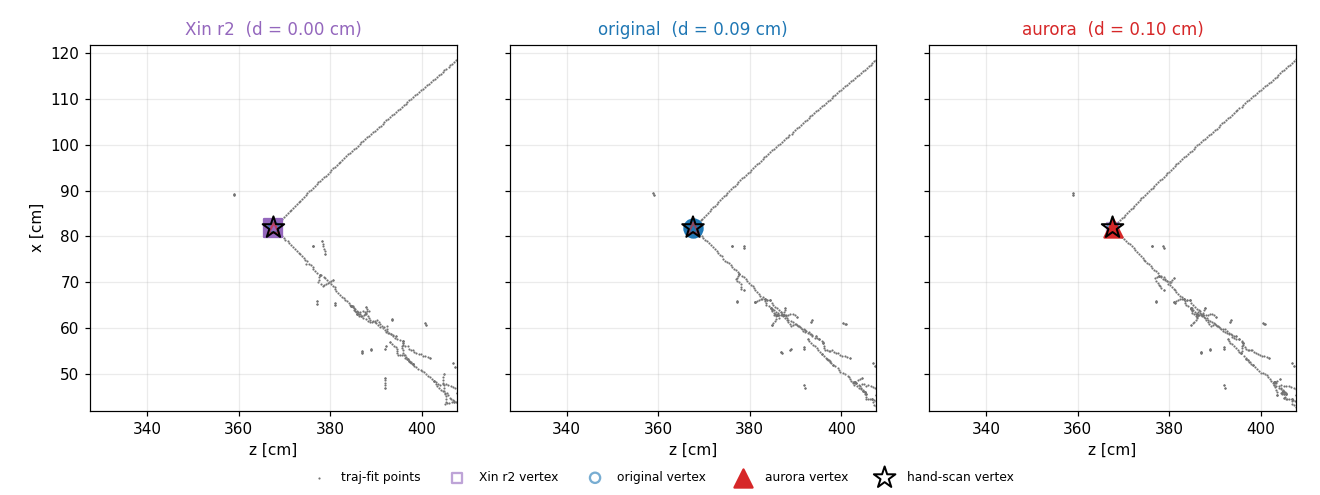
\includegraphics[width=0.92\linewidth]{figures/evt-18279-267597.png}\\[-2pt]
\scriptsize\raggedright
\textbf{Hand scan:} vertex (81.9, -128.9, 367.6) [Xin r2 vertex (scan Good/OK)], Xin r2 verdict: Good, flavor: $\nu_e$CC\\

\begin{tabular}{llcccc}
\toprule
method & & main vertex (x, y, z) cm & d to hand scan [cm] & $\nu_e$ / $\nu_\mu$ score & prediction \\
\midrule
Xin r2 & \href{https://www.phy.bnl.gov/twister/bee/set/9e2a1a1e-b637-4be5-99b7-f49bf8c04c57/event/29/}{Bee} & (81.9, -128.9, 367.6) & \textbf{0.00} & -- & -- \\
original & \href{https://www.phy.bnl.gov/twister/bee/set/89cdea53-c227-476c-8f67-0ae765f804b4/event/66/}{Bee} & (81.9, -128.9, 367.7) & \textbf{0.09} & 11.59 / 0.02 & $\nu_e$ \\
aurora & \href{https://www.phy.bnl.gov/twister/bee/set/431dc57f-997d-4cff-88e1-4e33fd743ab8/event/66/}{Bee} & (81.9, -128.9, 367.7) & \textbf{0.10} & 11.82 / -1.81 & $\nu_e$ \\
\bottomrule
\end{tabular}
\end{frame}

\begin{frame}{NC$\pi^0$-19: 18255/1/71372}
\vspace{-6pt}
\centering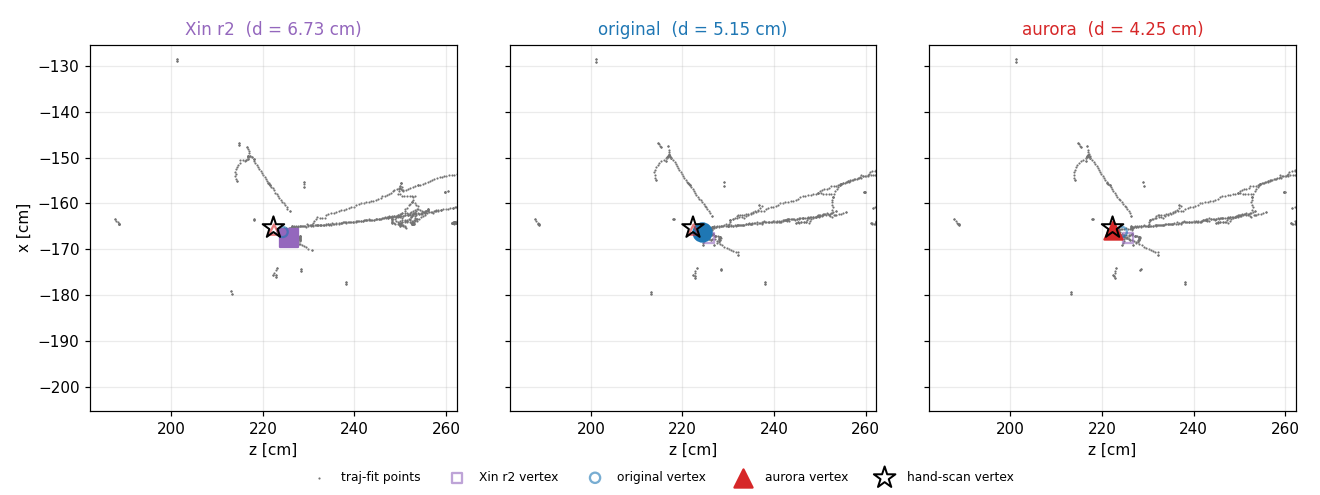
\includegraphics[width=0.92\linewidth]{figures/evt-18255-71372.png}\\[-2pt]
\scriptsize\raggedright
\textbf{Hand scan:} vertex (-165.3, -160.9, 222.3) [scanner point], Xin r2 verdict: Not good, flavor: NC$\pi^0$; \textcolor{red}{selection changes}\\
\textit{Scan note: close to (x, y, z) = (-165.3, -160.9, 222.3) EM shower messed up}\\
\begin{tabular}{llcccc}
\toprule
method & & main vertex (x, y, z) cm & d to hand scan [cm] & $\nu_e$ / $\nu_\mu$ score & prediction \\
\midrule
Xin r2 & \href{https://www.phy.bnl.gov/twister/bee/set/13900b8c-e48c-4ebb-8daa-da19e2e989b6/event/4/}{Bee} & (-167.5, -155.5, 225.7) & 6.73 & -- & -- \\
original & \href{https://www.phy.bnl.gov/twister/bee/set/89cdea53-c227-476c-8f67-0ae765f804b4/event/5/}{Bee} & (-166.2, -156.2, 224.3) & 5.15 & -15.00 / 1.80 & $\nu_\mu$CC \\
aurora & \href{https://www.phy.bnl.gov/twister/bee/set/431dc57f-997d-4cff-88e1-4e33fd743ab8/event/5/}{Bee} & (-165.7, -156.7, 222.4) & 4.25 & 0.87 / 0.51 & other \\
\bottomrule
\end{tabular}
\end{frame}

\begin{frame}{NC$\pi^0$-19: 18255/1/463565}
\vspace{-6pt}
\centering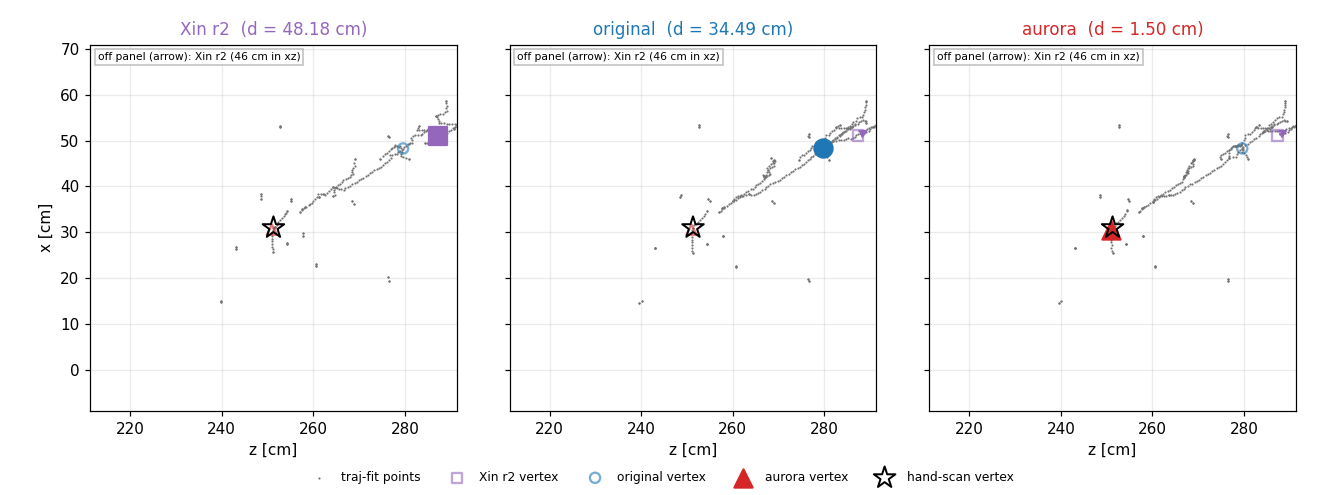
\includegraphics[width=0.92\linewidth]{figures/evt-18255-463565.png}\\[-2pt]
\scriptsize\raggedright
\textbf{Hand scan:} vertex (31.0, -141.8, 251.3) [scanner point], Xin r2 verdict: Not good, flavor: NC$\pi^0$\\
\textit{Scan note: close to (x, y, z) = (31.0, -141.8, 251.3)}\\
\begin{tabular}{llcccc}
\toprule
method & & main vertex (x, y, z) cm & d to hand scan [cm] & $\nu_e$ / $\nu_\mu$ score & prediction \\
\midrule
Xin r2 & \href{https://www.phy.bnl.gov/twister/bee/set/13900b8c-e48c-4ebb-8daa-da19e2e989b6/event/15/}{Bee} & (53.4, -127.1, 291.4) & 48.18 & -- & -- \\
original & \href{https://www.phy.bnl.gov/twister/bee/set/89cdea53-c227-476c-8f67-0ae765f804b4/event/10/}{Bee} & (48.3, -132.4, 279.6) & 34.49 & -1.69 / -0.03 & other \\
aurora & \href{https://www.phy.bnl.gov/twister/bee/set/431dc57f-997d-4cff-88e1-4e33fd743ab8/event/10/}{Bee} & (30.6, -143.2, 251.0) & 1.50 & -15.00 / 0.42 & other \\
\bottomrule
\end{tabular}
\end{frame}

\begin{frame}{NC$\pi^0$-19: 18255/1/180801}
\vspace{-6pt}
\centering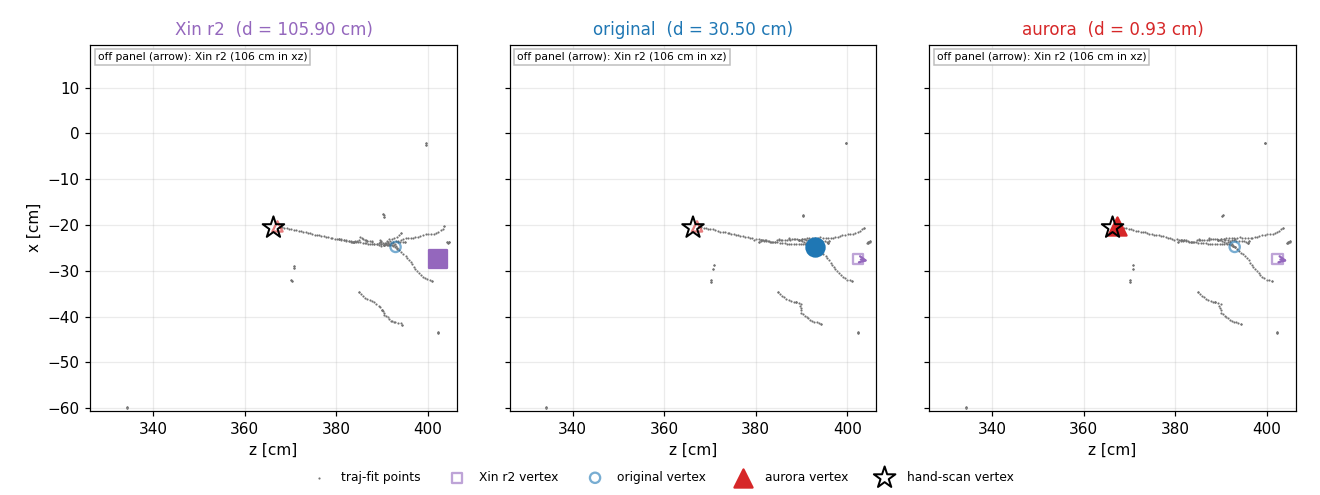
\includegraphics[width=0.92\linewidth]{figures/evt-18255-180801.png}\\[-2pt]
\scriptsize\raggedright
\textbf{Hand scan:} vertex (-20.6, -14.4, 366.3) [scanner point ?], Xin r2 verdict: Not good, flavor: NC$\pi^0$\\
\textit{Scan note: @(x, y, z) = (-20.6, -14.4, 366.3)?}\\
\begin{tabular}{llcccc}
\toprule
method & & main vertex (x, y, z) cm & d to hand scan [cm] & $\nu_e$ / $\nu_\mu$ score & prediction \\
\midrule
Xin r2 & \href{https://www.phy.bnl.gov/twister/bee/set/13900b8c-e48c-4ebb-8daa-da19e2e989b6/event/9/}{Bee} & (-40.3, -18.7, 470.3) & 105.90 & -- & -- \\
original & \href{https://www.phy.bnl.gov/twister/bee/set/89cdea53-c227-476c-8f67-0ae765f804b4/event/11/}{Bee} & (-24.8, -28.6, 393.0) & 30.50 & -15.00 / -0.10 & other \\
aurora & \href{https://www.phy.bnl.gov/twister/bee/set/431dc57f-997d-4cff-88e1-4e33fd743ab8/event/11/}{Bee} & (-20.3, -14.3, 367.2) & \textbf{0.93} & -15.00 / -0.42 & other \\
\bottomrule
\end{tabular}
\end{frame}

\begin{frame}{NC$\pi^0$-19: 18345/1/259542}
\vspace{-6pt}
\centering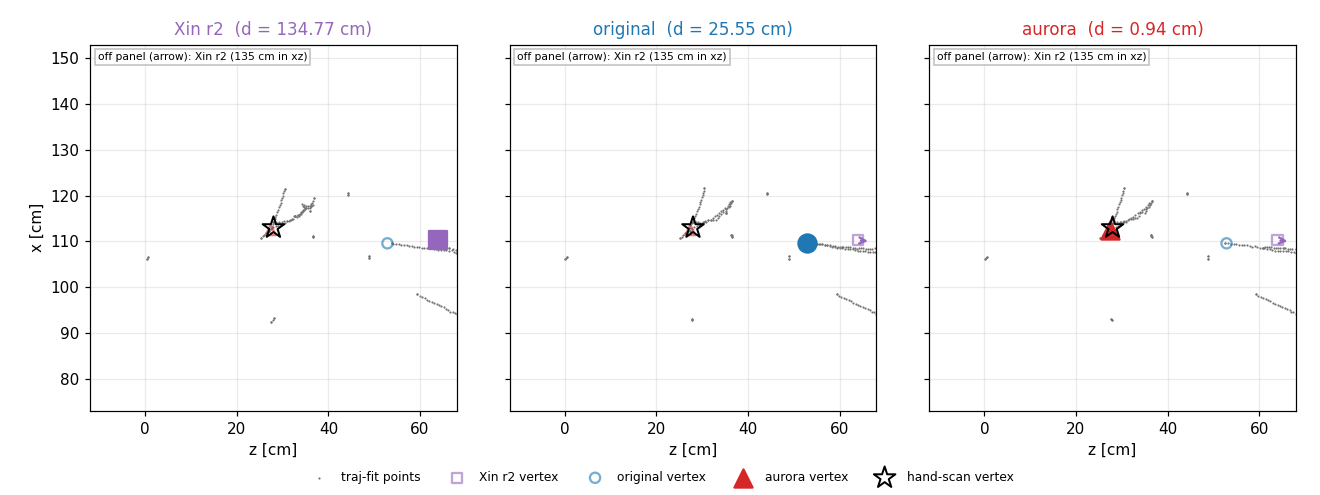
\includegraphics[width=0.92\linewidth]{figures/evt-18345-259542.png}\\[-2pt]
\scriptsize\raggedright
\textbf{Hand scan:} vertex (113.0, 15.0, 28.0) [scanner point], Xin r2 verdict: Not good, flavor: NC$\pi^0$\\
\textit{Scan note: close to (x,y,z) = (113, 15, 28)}\\
\begin{tabular}{llcccc}
\toprule
method & & main vertex (x, y, z) cm & d to hand scan [cm] & $\nu_e$ / $\nu_\mu$ score & prediction \\
\midrule
Xin r2 & \href{https://www.phy.bnl.gov/twister/bee/set/13900b8c-e48c-4ebb-8daa-da19e2e989b6/event/10/}{Bee} & (102.7, 18.4, 162.3) & 134.77 & -- & -- \\
original & \href{https://www.phy.bnl.gov/twister/bee/set/89cdea53-c227-476c-8f67-0ae765f804b4/event/12/}{Bee} & (109.6, 10.4, 52.9) & 25.55 & -15.00 / 0.38 & other \\
aurora & \href{https://www.phy.bnl.gov/twister/bee/set/431dc57f-997d-4cff-88e1-4e33fd743ab8/event/12/}{Bee} & (112.5, 15.5, 27.4) & \textbf{0.94} & -15.00 / 0.30 & other \\
\bottomrule
\end{tabular}
\end{frame}

\begin{frame}{NC$\pi^0$-19: 18255/1/56982}
\vspace{-6pt}
\centering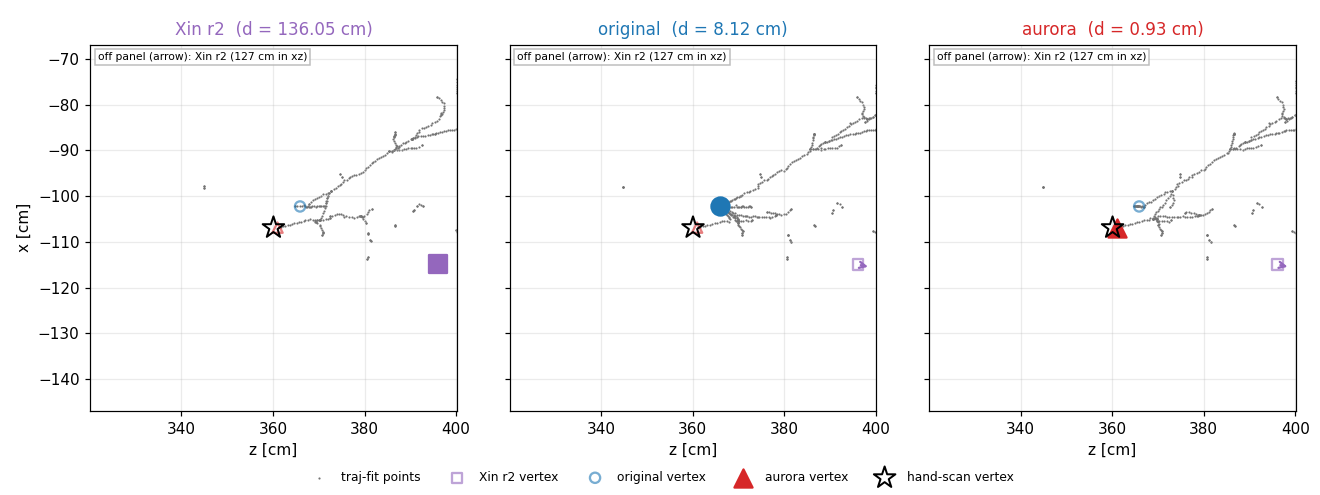
\includegraphics[width=0.92\linewidth]{figures/evt-18255-56982.png}\\[-2pt]
\scriptsize\raggedright
\textbf{Hand scan:} vertex (-106.9, -165.2, 360.1) [scanner point], Xin r2 verdict: Not Good, flavor: NC$\pi^0$\\
\textit{Scan note: @ (x, y, z) = (-106.9, -165.2, 360.1)}\\
\begin{tabular}{llcccc}
\toprule
method & & main vertex (x, y, z) cm & d to hand scan [cm] & $\nu_e$ / $\nu_\mu$ score & prediction \\
\midrule
Xin r2 & \href{https://www.phy.bnl.gov/twister/bee/set/13900b8c-e48c-4ebb-8daa-da19e2e989b6/event/3/}{Bee} & (-134.6, -117.4, 484.4) & 136.05 & -- & -- \\
original & \href{https://www.phy.bnl.gov/twister/bee/set/89cdea53-c227-476c-8f67-0ae765f804b4/event/13/}{Bee} & (-102.3, -168.5, 365.9) & 8.12 & 2.83 / 0.23 & other \\
aurora & \href{https://www.phy.bnl.gov/twister/bee/set/431dc57f-997d-4cff-88e1-4e33fd743ab8/event/13/}{Bee} & (-106.9, -165.5, 361.0) & \textbf{0.93} & -15.00 / 0.15 & other \\
\bottomrule
\end{tabular}
\end{frame}

\begin{frame}{NC$\pi^0$-19: 18345/1/21073}
\vspace{-6pt}
\centering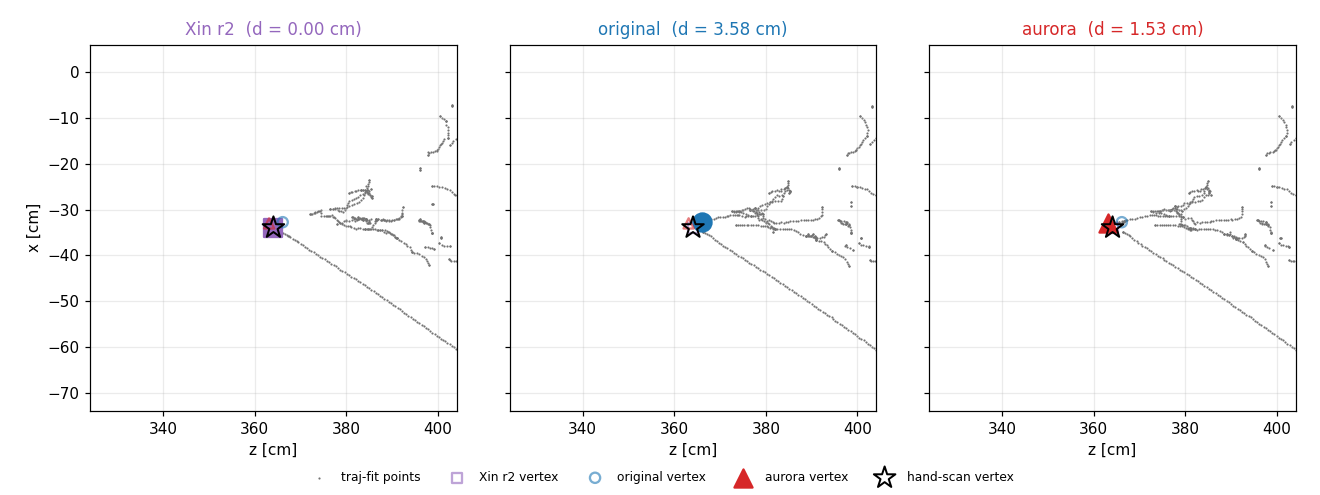
\includegraphics[width=0.92\linewidth]{figures/evt-18345-21073.png}\\[-2pt]
\scriptsize\raggedright
\textbf{Hand scan:} vertex (-34.0, 23.5, 364.1) [Xin r2 vertex (scan Good/OK)], Xin r2 verdict: Good, flavor: NC$\pi^0$\\
\textit{Scan note: track trajectory not covering entire em shower? improved}\\
\begin{tabular}{llcccc}
\toprule
method & & main vertex (x, y, z) cm & d to hand scan [cm] & $\nu_e$ / $\nu_\mu$ score & prediction \\
\midrule
Xin r2 & \href{https://www.phy.bnl.gov/twister/bee/set/13900b8c-e48c-4ebb-8daa-da19e2e989b6/event/1/}{Bee} & (-34.0, 23.5, 364.1) & \textbf{0.00} & -- & -- \\
original & \href{https://www.phy.bnl.gov/twister/bee/set/89cdea53-c227-476c-8f67-0ae765f804b4/event/15/}{Bee} & (-32.8, 26.2, 366.1) & 3.58 & -7.36 / 0.56 & other \\
aurora & \href{https://www.phy.bnl.gov/twister/bee/set/431dc57f-997d-4cff-88e1-4e33fd743ab8/event/15/}{Bee} & (-33.0, 24.2, 363.1) & 1.53 & -7.43 / -0.76 & other \\
\bottomrule
\end{tabular}
\end{frame}

\begin{frame}{NC$\pi^0$-19: 18259/1/105946}
\vspace{-6pt}
\centering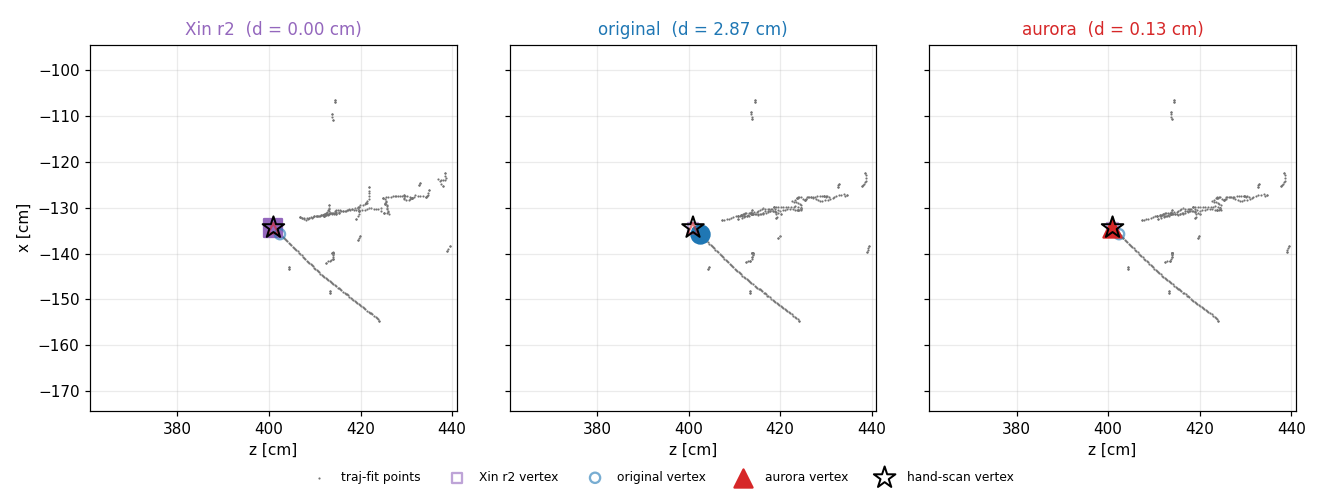
\includegraphics[width=0.92\linewidth]{figures/evt-18259-105946.png}\\[-2pt]
\scriptsize\raggedright
\textbf{Hand scan:} vertex (-134.3, -146.8, 401.0) [Xin r2 vertex (scan Good/OK)], Xin r2 verdict: Good, flavor: NC$\pi^0$\\
\textit{Scan note: Pi0 clustering issue}\\
\begin{tabular}{llcccc}
\toprule
method & & main vertex (x, y, z) cm & d to hand scan [cm] & $\nu_e$ / $\nu_\mu$ score & prediction \\
\midrule
Xin r2 & \href{https://www.phy.bnl.gov/twister/bee/set/13900b8c-e48c-4ebb-8daa-da19e2e989b6/event/6/}{Bee} & (-134.3, -146.8, 401.0) & \textbf{0.00} & -- & -- \\
original & \href{https://www.phy.bnl.gov/twister/bee/set/89cdea53-c227-476c-8f67-0ae765f804b4/event/16/}{Bee} & (-135.8, -148.9, 402.4) & 2.87 & -15.00 / -0.23 & other \\
aurora & \href{https://www.phy.bnl.gov/twister/bee/set/431dc57f-997d-4cff-88e1-4e33fd743ab8/event/16/}{Bee} & (-134.5, -146.9, 400.9) & \textbf{0.13} & -15.00 / -0.46 & other \\
\bottomrule
\end{tabular}
\end{frame}

\begin{frame}{NC$\pi^0$-19: 18255/1/142421}
\vspace{-6pt}
\centering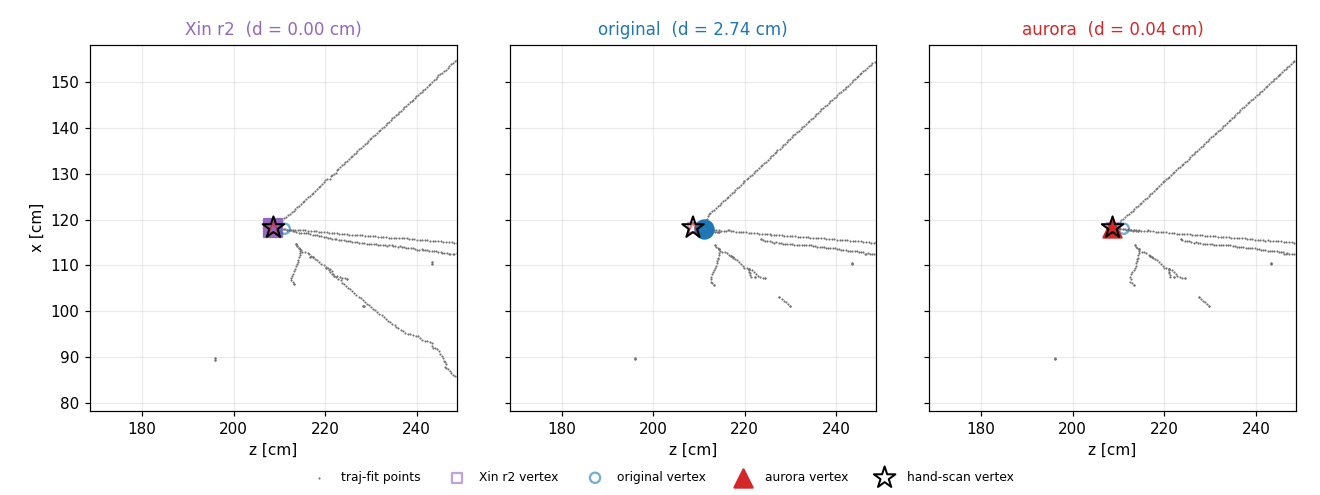
\includegraphics[width=0.92\linewidth]{figures/evt-18255-142421.png}\\[-2pt]
\scriptsize\raggedright
\textbf{Hand scan:} vertex (118.2, -70.2, 208.7) [Xin r2 vertex (scan Good/OK)], Xin r2 verdict: Good, flavor: NC$\pi^0$\\
\textit{Scan note: shower misided as track, gamma clustering}\\
\begin{tabular}{llcccc}
\toprule
method & & main vertex (x, y, z) cm & d to hand scan [cm] & $\nu_e$ / $\nu_\mu$ score & prediction \\
\midrule
Xin r2 & \href{https://www.phy.bnl.gov/twister/bee/set/13900b8c-e48c-4ebb-8daa-da19e2e989b6/event/8/}{Bee} & (118.2, -70.2, 208.7) & \textbf{0.00} & -- & -- \\
original & \href{https://www.phy.bnl.gov/twister/bee/set/89cdea53-c227-476c-8f67-0ae765f804b4/event/17/}{Bee} & (118.0, -69.0, 211.1) & 2.74 & -15.00 / 2.69 & $\nu_\mu$CC \\
aurora & \href{https://www.phy.bnl.gov/twister/bee/set/431dc57f-997d-4cff-88e1-4e33fd743ab8/event/17/}{Bee} & (118.3, -70.1, 208.7) & \textbf{0.04} & -15.00 / 2.87 & $\nu_\mu$CC \\
\bottomrule
\end{tabular}
\end{frame}

\begin{frame}{NC$\pi^0$-19: 18255/1/314838}
\vspace{-6pt}
\centering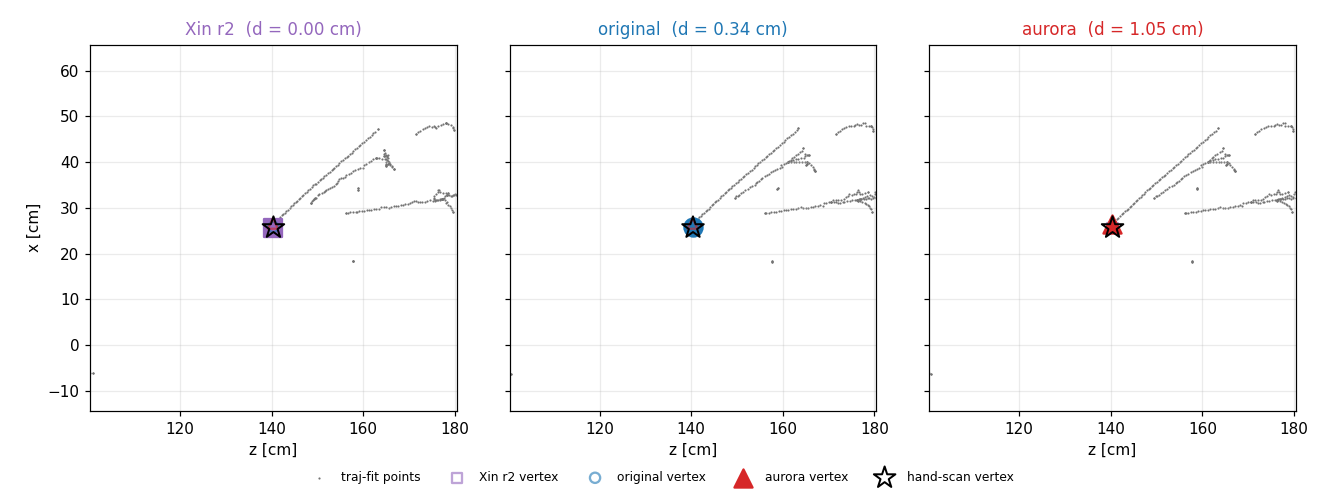
\includegraphics[width=0.92\linewidth]{figures/evt-18255-314838.png}\\[-2pt]
\scriptsize\raggedright
\textbf{Hand scan:} vertex (25.7, 155.3, 140.4) [Xin r2 vertex (scan Good/OK)], Xin r2 verdict: Good, flavor: NC$\pi^0$\\
\textit{Scan note: EM shower pi0 clustering issue}\\
\begin{tabular}{llcccc}
\toprule
method & & main vertex (x, y, z) cm & d to hand scan [cm] & $\nu_e$ / $\nu_\mu$ score & prediction \\
\midrule
Xin r2 & \href{https://www.phy.bnl.gov/twister/bee/set/13900b8c-e48c-4ebb-8daa-da19e2e989b6/event/12/}{Bee} & (25.7, 155.3, 140.4) & \textbf{0.00} & -- & -- \\
original & \href{https://www.phy.bnl.gov/twister/bee/set/89cdea53-c227-476c-8f67-0ae765f804b4/event/21/}{Bee} & (25.8, 155.0, 140.4) & \textbf{0.34} & -15.00 / -0.06 & other \\
aurora & \href{https://www.phy.bnl.gov/twister/bee/set/431dc57f-997d-4cff-88e1-4e33fd743ab8/event/21/}{Bee} & (26.6, 154.7, 140.3) & 1.05 & -15.00 / -0.62 & other \\
\bottomrule
\end{tabular}
\end{frame}

\begin{frame}{NC$\pi^0$-19: 18259/1/18625}
\vspace{-6pt}
\centering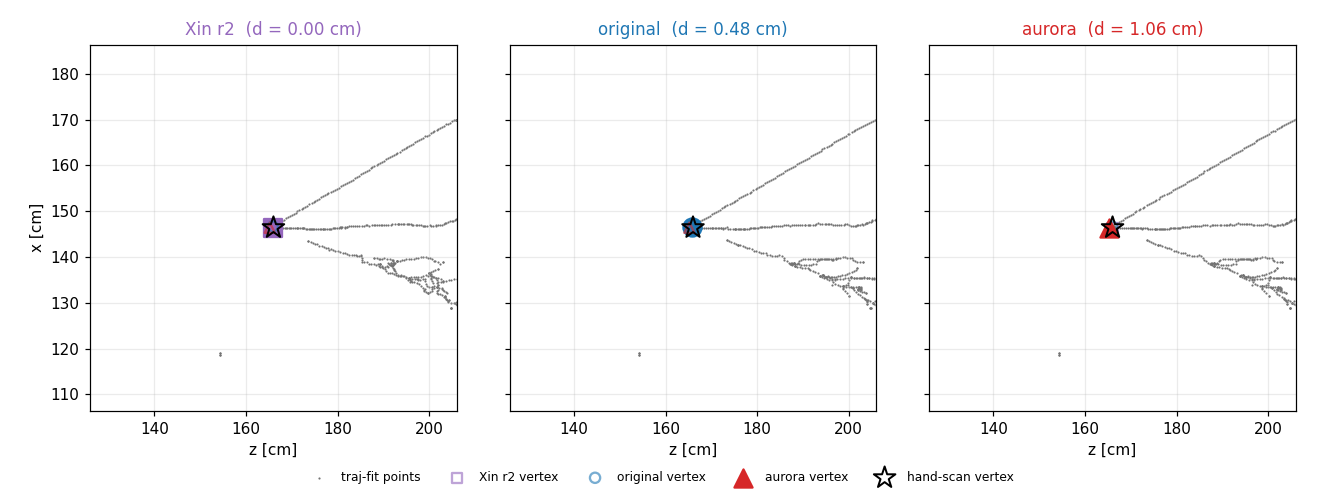
\includegraphics[width=0.92\linewidth]{figures/evt-18259-18625.png}\\[-2pt]
\scriptsize\raggedright
\textbf{Hand scan:} vertex (146.4, 84.9, 166.0) [Xin r2 vertex (scan Good/OK)], Xin r2 verdict: Good, flavor: NC$\pi^0$\\
\textit{Scan note: still missing clustering points @ (x, y, z) = (142.1, 78.3, 176.5)}\\
\begin{tabular}{llcccc}
\toprule
method & & main vertex (x, y, z) cm & d to hand scan [cm] & $\nu_e$ / $\nu_\mu$ score & prediction \\
\midrule
Xin r2 & \href{https://www.phy.bnl.gov/twister/bee/set/13900b8c-e48c-4ebb-8daa-da19e2e989b6/event/0/}{Bee} & (146.4, 84.9, 166.0) & \textbf{0.00} & -- & -- \\
original & \href{https://www.phy.bnl.gov/twister/bee/set/89cdea53-c227-476c-8f67-0ae765f804b4/event/22/}{Bee} & (146.7, 84.5, 165.8) & \textbf{0.48} & -15.00 / 0.59 & other \\
aurora & \href{https://www.phy.bnl.gov/twister/bee/set/431dc57f-997d-4cff-88e1-4e33fd743ab8/event/22/}{Bee} & (146.4, 84.2, 165.2) & 1.06 & -15.00 / 0.70 & other \\
\bottomrule
\end{tabular}
\end{frame}

\begin{frame}{NC$\pi^0$-19: 18255/1/506746}
\vspace{-6pt}
\centering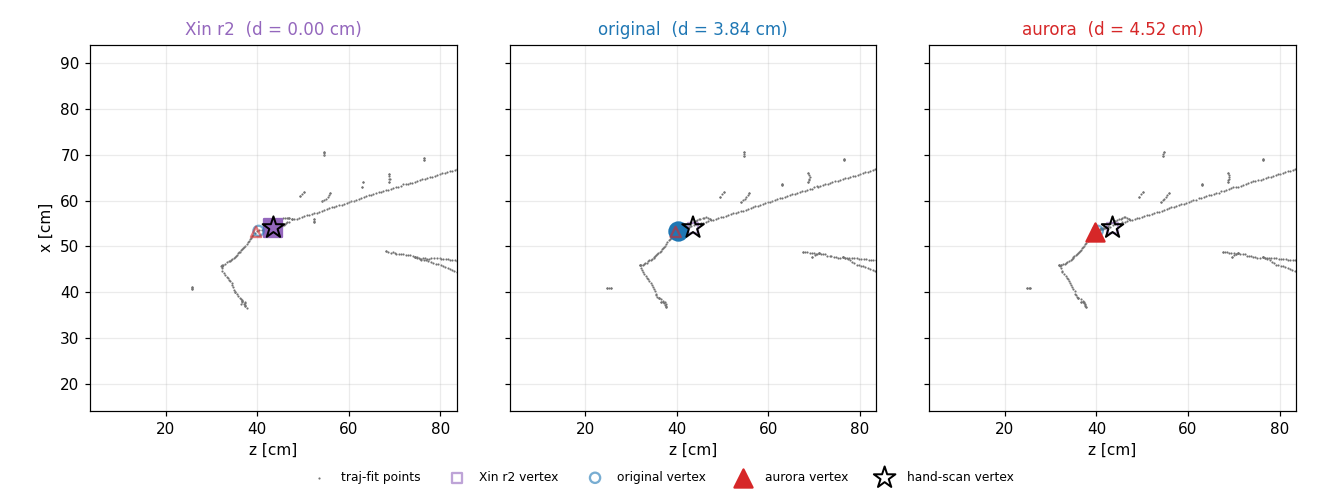
\includegraphics[width=0.92\linewidth]{figures/evt-18255-506746.png}\\[-2pt]
\scriptsize\raggedright
\textbf{Hand scan:} vertex (54.1, -10.7, 43.5) [Xin r2 vertex (scan Good/OK)], Xin r2 verdict: OK, flavor: NC$\pi^0$\\
\textit{Scan note: PR @ vertex needs improvements}\\
\begin{tabular}{llcccc}
\toprule
method & & main vertex (x, y, z) cm & d to hand scan [cm] & $\nu_e$ / $\nu_\mu$ score & prediction \\
\midrule
Xin r2 & \href{https://www.phy.bnl.gov/twister/bee/set/13900b8c-e48c-4ebb-8daa-da19e2e989b6/event/17/}{Bee} & (54.1, -10.7, 43.5) & \textbf{0.00} & -- & -- \\
original & \href{https://www.phy.bnl.gov/twister/bee/set/89cdea53-c227-476c-8f67-0ae765f804b4/event/23/}{Bee} & (53.4, -12.6, 40.3) & 3.84 & -15.00 / 0.58 & other \\
aurora & \href{https://www.phy.bnl.gov/twister/bee/set/431dc57f-997d-4cff-88e1-4e33fd743ab8/event/23/}{Bee} & (53.1, -13.0, 39.7) & 4.52 & -15.00 / 0.51 & other \\
\bottomrule
\end{tabular}
\end{frame}

\begin{frame}{NC$\pi^0$-19: 18261/1/285567}
\vspace{-6pt}
\centering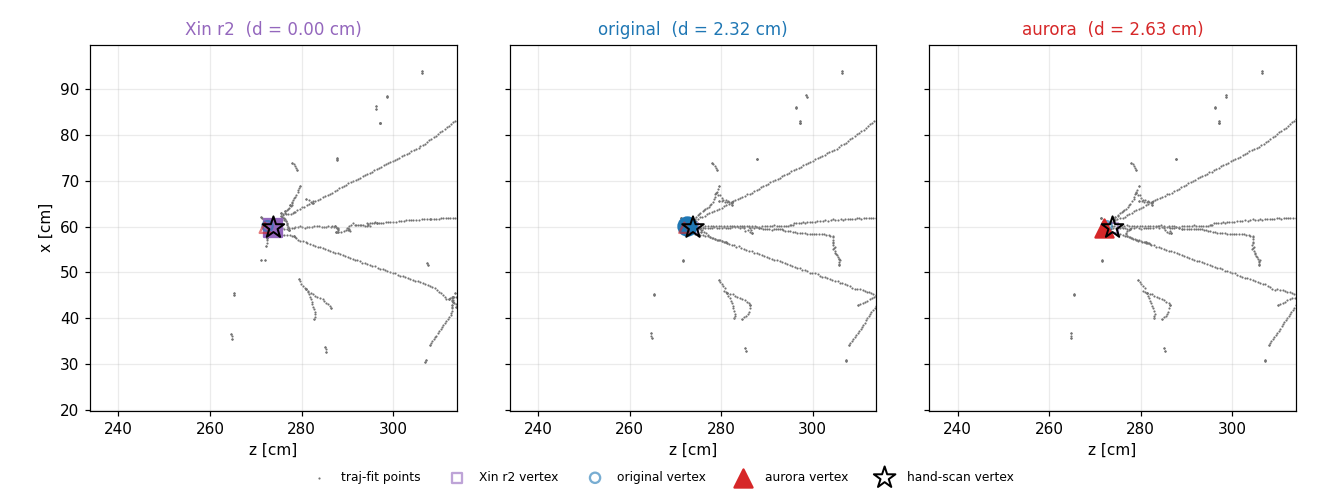
\includegraphics[width=0.92\linewidth]{figures/evt-18261-285567.png}\\[-2pt]
\scriptsize\raggedright
\textbf{Hand scan:} vertex (59.8, -176.4, 273.9) [Xin r2 vertex (scan Good/OK)], Xin r2 verdict: OK, flavor: NC$\pi^0$\\
\textit{Scan note: Vertex PR issues}\\
\begin{tabular}{llcccc}
\toprule
method & & main vertex (x, y, z) cm & d to hand scan [cm] & $\nu_e$ / $\nu_\mu$ score & prediction \\
\midrule
Xin r2 & \href{https://www.phy.bnl.gov/twister/bee/set/13900b8c-e48c-4ebb-8daa-da19e2e989b6/event/11/}{Bee} & (59.8, -176.4, 273.9) & \textbf{0.00} & -- & -- \\
original & \href{https://www.phy.bnl.gov/twister/bee/set/89cdea53-c227-476c-8f67-0ae765f804b4/event/24/}{Bee} & (60.1, -178.3, 272.6) & 2.32 & -7.23 / 0.79 & other \\
aurora & \href{https://www.phy.bnl.gov/twister/bee/set/431dc57f-997d-4cff-88e1-4e33fd743ab8/event/24/}{Bee} & (59.8, -178.2, 272.0) & 2.63 & -6.52 / -0.01 & other \\
\bottomrule
\end{tabular}
\end{frame}

\begin{frame}{NC$\pi^0$-19: 18255/1/114446}
\vspace{-6pt}
\centering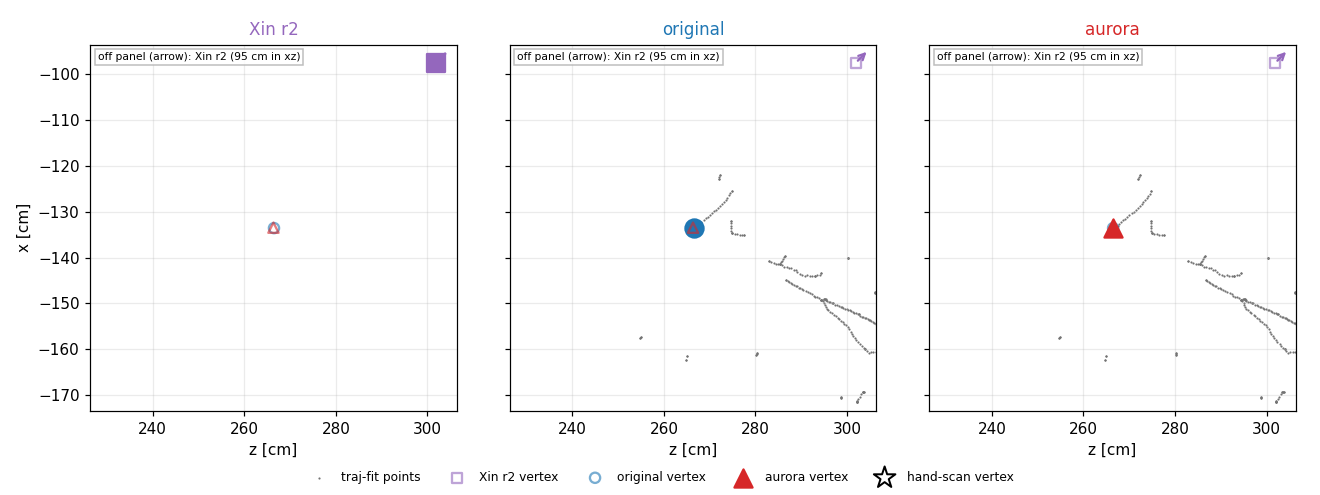
\includegraphics[width=0.92\linewidth]{figures/evt-18255-114446.png}\\[-2pt]
\scriptsize\raggedright
\textbf{Hand scan:} vertex (-65.9, -64.4, 333.1) [Xin r2 vertex (scan Good/OK)], Xin r2 verdict: OK, flavor: NC$\pi^0$; \textcolor{orange!80!black}{our candidate $\ne$ scanned interaction}\\
\textit{Scan note: QL mismatch}\\
\begin{tabular}{llcccc}
\toprule
method & & main vertex (x, y, z) cm & d to hand scan [cm] & $\nu_e$ / $\nu_\mu$ score & prediction \\
\midrule
Xin r2 & \href{https://www.phy.bnl.gov/twister/bee/set/13900b8c-e48c-4ebb-8daa-da19e2e989b6/event/7/}{Bee} & (-65.9, -64.4, 333.1) & -- & -- & -- \\
original & \href{https://www.phy.bnl.gov/twister/bee/set/89cdea53-c227-476c-8f67-0ae765f804b4/event/34/}{Bee} & (-133.6, -92.4, 266.5) & -- & -15.00 / -0.64 & other \\
aurora & \href{https://www.phy.bnl.gov/twister/bee/set/431dc57f-997d-4cff-88e1-4e33fd743ab8/event/34/}{Bee} & (-133.5, -91.9, 266.4) & -- & -15.00 / -0.72 & other \\
\bottomrule
\end{tabular}
\end{frame}

\begin{frame}{NC$\pi^0$-19: 18255/1/521075}
\vspace{-6pt}
\centering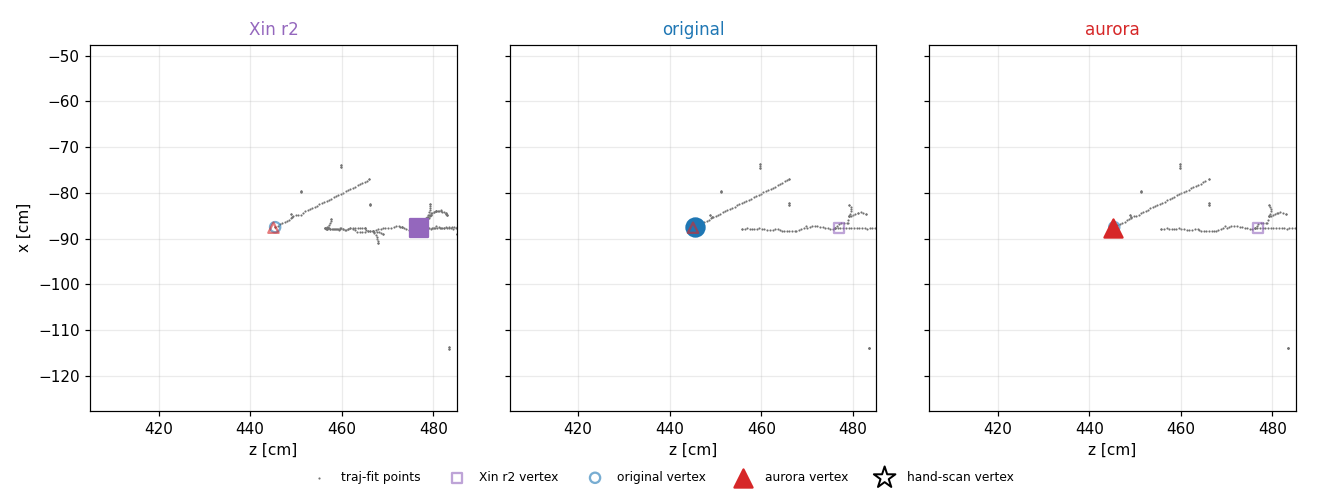
\includegraphics[width=0.92\linewidth]{figures/evt-18255-521075.png}\\[-2pt]
\scriptsize\raggedright
\textbf{Hand scan:} vertex (-177.2, 20.4, 378.8) [scanner point], Xin r2 verdict: Not good, flavor: NC$\pi^0$; \textcolor{orange!80!black}{our candidate $\ne$ scanned interaction}\\
\textit{Scan note: close to (x, y, z) = (-177.2, 20.4, 378.8)}\\
\begin{tabular}{llcccc}
\toprule
method & & main vertex (x, y, z) cm & d to hand scan [cm] & $\nu_e$ / $\nu_\mu$ score & prediction \\
\midrule
Xin r2 & \href{https://www.phy.bnl.gov/twister/bee/set/13900b8c-e48c-4ebb-8daa-da19e2e989b6/event/18/}{Bee} & (-87.6, -36.6, 476.9) & -- & -- & -- \\
original & \href{https://www.phy.bnl.gov/twister/bee/set/89cdea53-c227-476c-8f67-0ae765f804b4/event/37/}{Bee} & (-87.5, -35.4, 445.5) & -- & -15.00 / -0.42 & other \\
aurora & \href{https://www.phy.bnl.gov/twister/bee/set/431dc57f-997d-4cff-88e1-4e33fd743ab8/event/37/}{Bee} & (-87.6, -35.5, 445.1) & -- & -15.00 / -0.79 & other \\
\bottomrule
\end{tabular}
\end{frame}

\begin{frame}{NC$\pi^0$-19: 18259/1/37112}
\vspace{-6pt}
\centering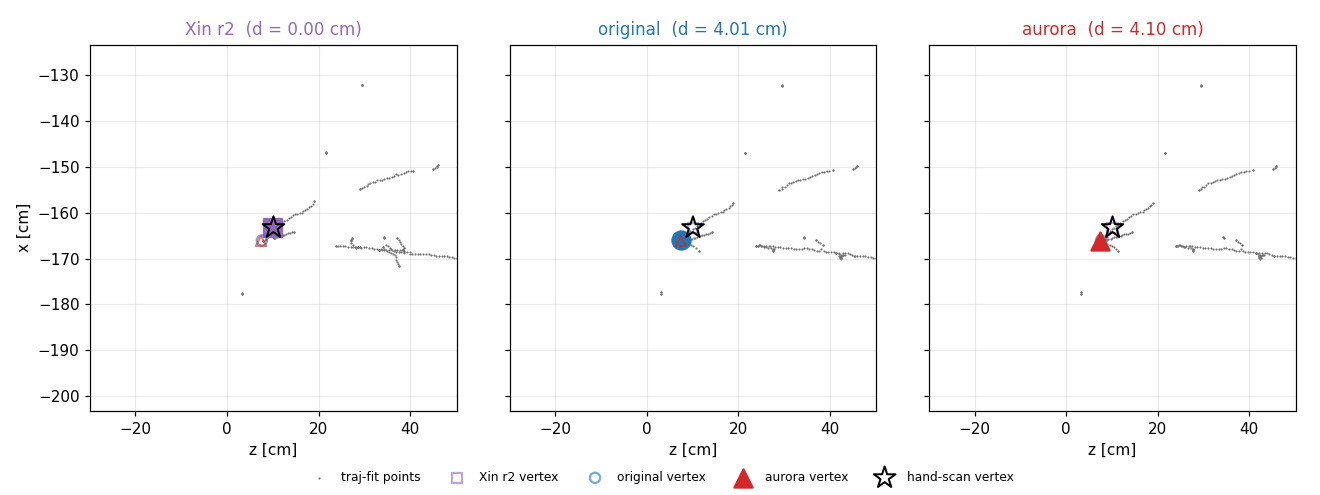
\includegraphics[width=0.92\linewidth]{figures/evt-18259-37112.png}\\[-2pt]
\scriptsize\raggedright
\textbf{Hand scan:} vertex (-163.3, 73.3, 10.1) [Xin r2 vertex (scan Good/OK)], Xin r2 verdict: OK, flavor: NC$\pi^0$\\
\textit{Scan note: PR @ vertex not ideal}\\
\begin{tabular}{llcccc}
\toprule
method & & main vertex (x, y, z) cm & d to hand scan [cm] & $\nu_e$ / $\nu_\mu$ score & prediction \\
\midrule
Xin r2 & \href{https://www.phy.bnl.gov/twister/bee/set/13900b8c-e48c-4ebb-8daa-da19e2e989b6/event/2/}{Bee} & (-163.3, 73.3, 10.1) & \textbf{0.00} & -- & -- \\
original & \href{https://www.phy.bnl.gov/twister/bee/set/89cdea53-c227-476c-8f67-0ae765f804b4/event/42/}{Bee} & (-166.1, 71.9, 7.6) & 4.01 & -2.75 / 0.64 & other \\
aurora & \href{https://www.phy.bnl.gov/twister/bee/set/431dc57f-997d-4cff-88e1-4e33fd743ab8/event/42/}{Bee} & (-166.1, 72.2, 7.4) & 4.10 & -1.70 / 0.63 & other \\
\bottomrule
\end{tabular}
\end{frame}

\begin{frame}{NC$\pi^0$-19: 18255/1/359980}
\vspace{-6pt}
\centering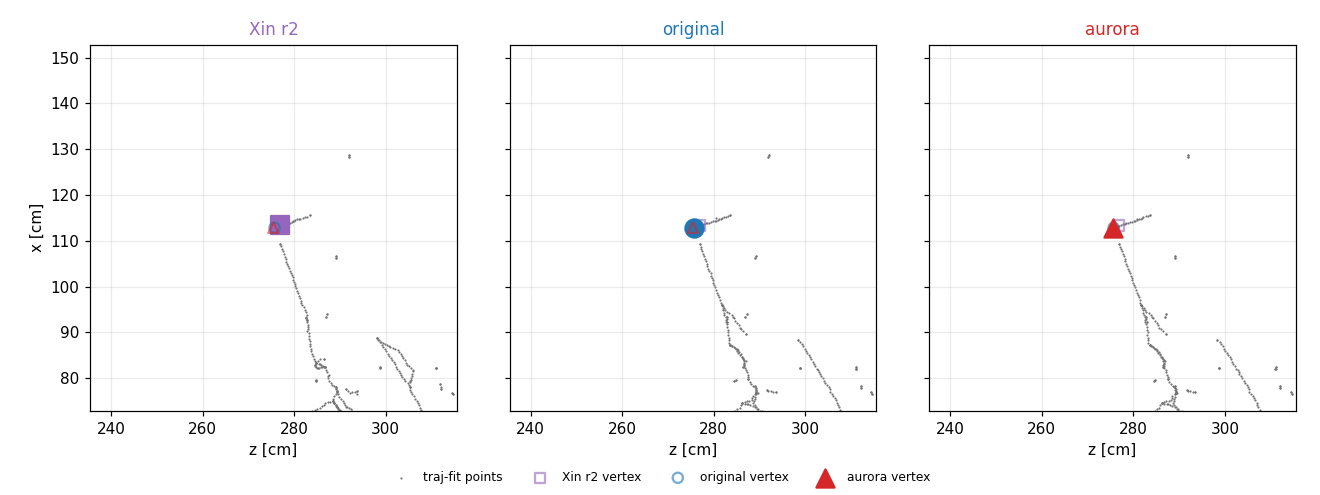
\includegraphics[width=0.92\linewidth]{figures/evt-18255-359980.png}\\[-2pt]
\scriptsize\raggedright
\textbf{Hand scan:} vertex -- [none], Xin r2 verdict: Not good, flavor: NC$\pi^0$\\
\textit{Scan note: proton not ided???}\\
\begin{tabular}{llcccc}
\toprule
method & & main vertex (x, y, z) cm & d to hand scan [cm] & $\nu_e$ / $\nu_\mu$ score & prediction \\
\midrule
Xin r2 & \href{https://www.phy.bnl.gov/twister/bee/set/13900b8c-e48c-4ebb-8daa-da19e2e989b6/event/13/}{Bee} & (113.4, 157.7, 276.9) & -- & -- & -- \\
original & \href{https://www.phy.bnl.gov/twister/bee/set/89cdea53-c227-476c-8f67-0ae765f804b4/event/45/}{Bee} & (112.9, 155.9, 275.7) & -- & -15.00 / -1.12 & other \\
aurora & \href{https://www.phy.bnl.gov/twister/bee/set/431dc57f-997d-4cff-88e1-4e33fd743ab8/event/45/}{Bee} & (112.9, 155.8, 275.5) & -- & -15.00 / -1.30 & other \\
\bottomrule
\end{tabular}
\end{frame}

\begin{frame}{NC$\pi^0$-19: 18255/1/506114}
\vspace{-6pt}
\centering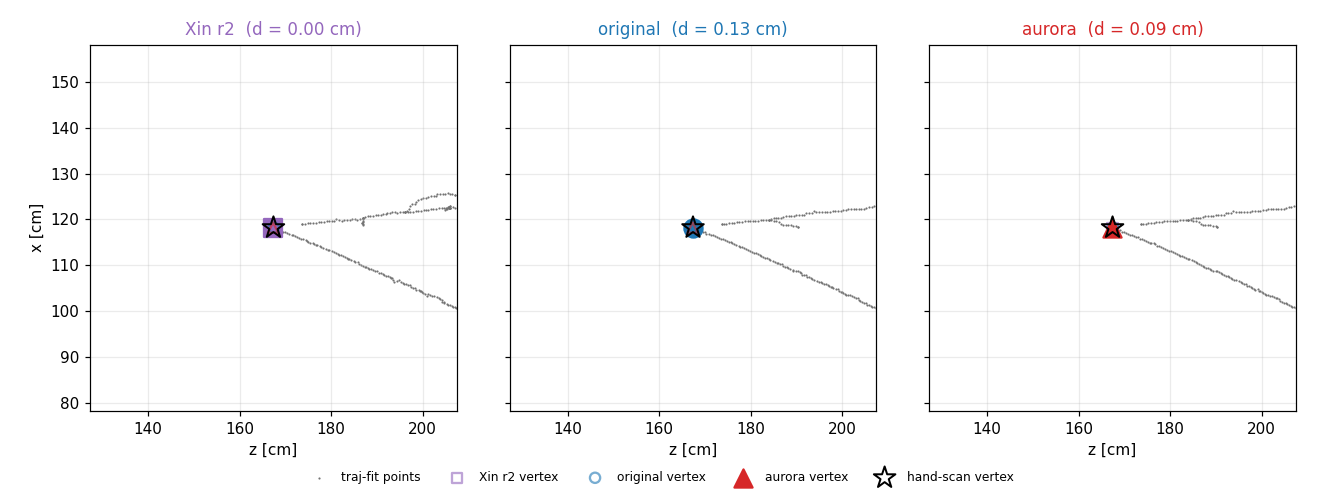
\includegraphics[width=0.92\linewidth]{figures/evt-18255-506114.png}\\[-2pt]
\scriptsize\raggedright
\textbf{Hand scan:} vertex (118.2, -13.9, 167.4) [Xin r2 vertex (scan Good/OK)], Xin r2 verdict: Good, flavor: NC$\pi^0$\\
\textit{Scan note: QL matching}\\
\begin{tabular}{llcccc}
\toprule
method & & main vertex (x, y, z) cm & d to hand scan [cm] & $\nu_e$ / $\nu_\mu$ score & prediction \\
\midrule
Xin r2 & \href{https://www.phy.bnl.gov/twister/bee/set/13900b8c-e48c-4ebb-8daa-da19e2e989b6/event/16/}{Bee} & (118.2, -13.9, 167.4) & \textbf{0.00} & -- & -- \\
original & \href{https://www.phy.bnl.gov/twister/bee/set/89cdea53-c227-476c-8f67-0ae765f804b4/event/48/}{Bee} & (118.2, -13.8, 167.5) & \textbf{0.13} & -15.00 / -0.92 & other \\
aurora & \href{https://www.phy.bnl.gov/twister/bee/set/431dc57f-997d-4cff-88e1-4e33fd743ab8/event/48/}{Bee} & (118.2, -13.9, 167.3) & \textbf{0.09} & -15.00 / -0.92 & other \\
\bottomrule
\end{tabular}
\end{frame}

\begin{frame}{NC$\pi^0$-19: 18364/1/84229}
\vspace{-6pt}
\centering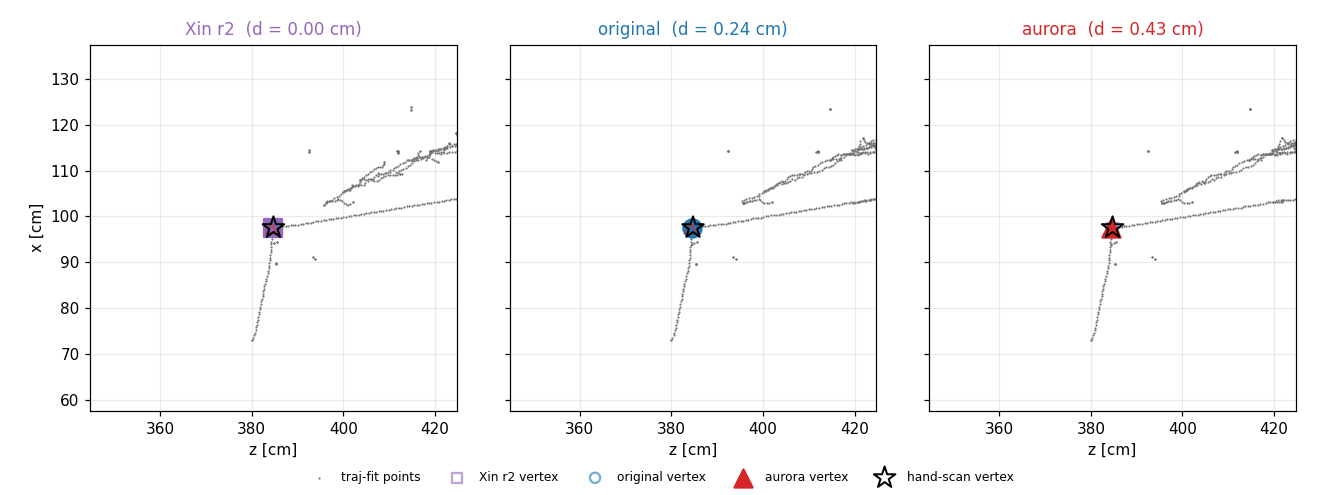
\includegraphics[width=0.92\linewidth]{figures/evt-18364-84229.png}\\[-2pt]
\scriptsize\raggedright
\textbf{Hand scan:} vertex (97.5, 122.7, 384.7) [Xin r2 vertex (scan Good/OK)], Xin r2 verdict: Good, flavor: NC$\pi^0$\\
\textit{Scan note: Pi0 clustering issue}\\
\begin{tabular}{llcccc}
\toprule
method & & main vertex (x, y, z) cm & d to hand scan [cm] & $\nu_e$ / $\nu_\mu$ score & prediction \\
\midrule
Xin r2 & \href{https://www.phy.bnl.gov/twister/bee/set/13900b8c-e48c-4ebb-8daa-da19e2e989b6/event/5/}{Bee} & (97.5, 122.7, 384.7) & \textbf{0.00} & -- & -- \\
original & \href{https://www.phy.bnl.gov/twister/bee/set/89cdea53-c227-476c-8f67-0ae765f804b4/event/50/}{Bee} & (97.5, 122.7, 384.5) & \textbf{0.24} & -15.00 / 0.50 & other \\
aurora & \href{https://www.phy.bnl.gov/twister/bee/set/431dc57f-997d-4cff-88e1-4e33fd743ab8/event/50/}{Bee} & (97.4, 122.8, 384.3) & \textbf{0.43} & -15.00 / 0.86 & other \\
\bottomrule
\end{tabular}
\end{frame}

\begin{frame}{NC$\pi^0$-19: 18255/1/399860}
\vspace{-6pt}
\centering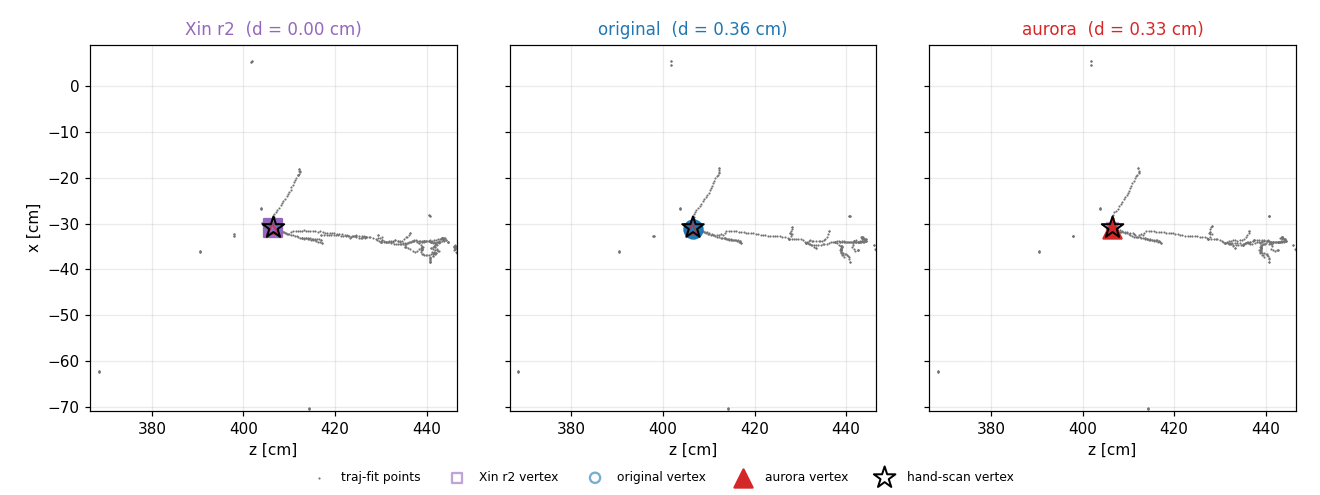
\includegraphics[width=0.92\linewidth]{figures/evt-18255-399860.png}\\[-2pt]
\scriptsize\raggedright
\textbf{Hand scan:} vertex (-30.9, -84.6, 406.5) [Xin r2 vertex (scan Good/OK)], Xin r2 verdict: Good, flavor: NC$\pi^0$\\
\textit{Scan note: one track merged to shower?}\\
\begin{tabular}{llcccc}
\toprule
method & & main vertex (x, y, z) cm & d to hand scan [cm] & $\nu_e$ / $\nu_\mu$ score & prediction \\
\midrule
Xin r2 & \href{https://www.phy.bnl.gov/twister/bee/set/13900b8c-e48c-4ebb-8daa-da19e2e989b6/event/14/}{Bee} & (-30.9, -84.6, 406.5) & \textbf{0.00} & -- & -- \\
original & \href{https://www.phy.bnl.gov/twister/bee/set/89cdea53-c227-476c-8f67-0ae765f804b4/event/55/}{Bee} & (-31.1, -84.3, 406.5) & \textbf{0.36} & 9.00 / -0.89 & $\nu_e$ \\
aurora & \href{https://www.phy.bnl.gov/twister/bee/set/431dc57f-997d-4cff-88e1-4e33fd743ab8/event/55/}{Bee} & (-31.1, -84.4, 406.4) & \textbf{0.33} & 10.53 / -0.11 & $\nu_e$ \\
\bottomrule
\end{tabular}
\end{frame}

\end{document}